\documentclass[twoside]{book}

% Packages required by doxygen
\usepackage{fixltx2e}
\usepackage{calc}
\usepackage{doxygen}
\usepackage[export]{adjustbox} % also loads graphicx
\usepackage{graphicx}
\usepackage[utf8]{inputenc}
\usepackage{makeidx}
\usepackage{multicol}
\usepackage{multirow}
\PassOptionsToPackage{warn}{textcomp}
\usepackage{textcomp}
\usepackage[nointegrals]{wasysym}
\usepackage[table]{xcolor}

% Font selection
\usepackage[T1]{fontenc}
\usepackage[scaled=.90]{helvet}
\usepackage{courier}
\usepackage{amssymb}
\usepackage{sectsty}
\renewcommand{\familydefault}{\sfdefault}
\allsectionsfont{%
  \fontseries{bc}\selectfont%
  \color{darkgray}%
}
\renewcommand{\DoxyLabelFont}{%
  \fontseries{bc}\selectfont%
  \color{darkgray}%
}
\newcommand{\+}{\discretionary{\mbox{\scriptsize$\hookleftarrow$}}{}{}}

% Page & text layout
\usepackage{geometry}
\geometry{%
  a4paper,%
  top=2.5cm,%
  bottom=2.5cm,%
  left=2.5cm,%
  right=2.5cm%
}
\tolerance=750
\hfuzz=15pt
\hbadness=750
\setlength{\emergencystretch}{15pt}
\setlength{\parindent}{0cm}
\setlength{\parskip}{0.2cm}
\makeatletter
\renewcommand{\paragraph}{%
  \@startsection{paragraph}{4}{0ex}{-1.0ex}{1.0ex}{%
    \normalfont\normalsize\bfseries\SS@parafont%
  }%
}
\renewcommand{\subparagraph}{%
  \@startsection{subparagraph}{5}{0ex}{-1.0ex}{1.0ex}{%
    \normalfont\normalsize\bfseries\SS@subparafont%
  }%
}
\makeatother

% Headers & footers
\usepackage{fancyhdr}
\pagestyle{fancyplain}
\fancyhead[LE]{\fancyplain{}{\bfseries\thepage}}
\fancyhead[CE]{\fancyplain{}{}}
\fancyhead[RE]{\fancyplain{}{\bfseries\leftmark}}
\fancyhead[LO]{\fancyplain{}{\bfseries\rightmark}}
\fancyhead[CO]{\fancyplain{}{}}
\fancyhead[RO]{\fancyplain{}{\bfseries\thepage}}
\fancyfoot[LE]{\fancyplain{}{}}
\fancyfoot[CE]{\fancyplain{}{}}
\fancyfoot[RE]{\fancyplain{}{\bfseries\scriptsize Generated on Tue May 5 2015 09\+:31\+:43 for A\+I\+S\+\_\+\+Tracking\+\_\+\+And\+\_\+\+Detection by Doxygen }}
\fancyfoot[LO]{\fancyplain{}{\bfseries\scriptsize Generated on Tue May 5 2015 09\+:31\+:43 for A\+I\+S\+\_\+\+Tracking\+\_\+\+And\+\_\+\+Detection by Doxygen }}
\fancyfoot[CO]{\fancyplain{}{}}
\fancyfoot[RO]{\fancyplain{}{}}
\renewcommand{\footrulewidth}{0.4pt}
\renewcommand{\chaptermark}[1]{%
  \markboth{#1}{}%
}
\renewcommand{\sectionmark}[1]{%
  \markright{\thesection\ #1}%
}

% Indices & bibliography
\usepackage{natbib}
\usepackage[titles]{tocloft}
\setcounter{tocdepth}{3}
\setcounter{secnumdepth}{5}
\makeindex

% Hyperlinks (required, but should be loaded last)
\usepackage{ifpdf}
\ifpdf
  \usepackage[pdftex,pagebackref=true]{hyperref}
\else
  \usepackage[ps2pdf,pagebackref=true]{hyperref}
\fi
\hypersetup{%
  colorlinks=true,%
  linkcolor=blue,%
  citecolor=blue,%
  unicode%
}

% Custom commands
\newcommand{\clearemptydoublepage}{%
  \newpage{\pagestyle{empty}\cleardoublepage}%
}


%===== C O N T E N T S =====

\begin{document}

% Titlepage & ToC
\hypersetup{pageanchor=false,
             bookmarks=true,
             bookmarksnumbered=true,
             pdfencoding=unicode
            }
\pagenumbering{roman}
\begin{titlepage}
\vspace*{7cm}
\begin{center}%
{\Large A\+I\+S\+\_\+\+Tracking\+\_\+\+And\+\_\+\+Detection }\\
\vspace*{1cm}
{\large Generated by Doxygen 1.8.9.1}\\
\vspace*{0.5cm}
{\small Tue May 5 2015 09:31:43}\\
\end{center}
\end{titlepage}
\clearemptydoublepage
\tableofcontents
\clearemptydoublepage
\pagenumbering{arabic}
\hypersetup{pageanchor=true}

%--- Begin generated contents ---
\chapter{Main Page}
\label{index}\hypertarget{index}{}\hypertarget{index_intro_sec}{}\section{Introduction}\label{index_intro_sec}
The A\+I\+S tracking and detection software was created for my(Helen Harman\textquotesingle{}s) dissertation project.\hypertarget{index_contact_sec}{}\section{Contact}\label{index_contact_sec}
Helen Harman (\href{mailto:heh14@aber.ac.uk}{\tt heh14@aber.\+ac.\+uk}) Aberystwyth University M\+Eng Software Engineering Student. 
\chapter{Hierarchical Index}
\section{Class Hierarchy}
This inheritance list is sorted roughly, but not completely, alphabetically\+:\begin{DoxyCompactList}
\item \contentsline{section}{A\+R\+B}{\pageref{class_a_r_b}}{}
\item \contentsline{section}{Distance\+Base}{\pageref{class_distance_base}}{}
\begin{DoxyCompactList}
\item \contentsline{section}{Euclidean\+Distance}{\pageref{class_euclidean_distance}}{}
\item \contentsline{section}{Sum\+Of\+Squared\+Difference}{\pageref{class_sum_of_squared_difference}}{}
\end{DoxyCompactList}
\item \contentsline{section}{A\+I\+S\+\_\+\+Options\+:\+:Location}{\pageref{struct_a_i_s___options_1_1_location}}{}
\item \contentsline{section}{Network}{\pageref{class_network}}{}
\item \contentsline{section}{Output\+Data}{\pageref{class_output_data}}{}
\item Q\+Main\+Window\begin{DoxyCompactList}
\item \contentsline{section}{Main\+Window}{\pageref{class_main_window}}{}
\end{DoxyCompactList}
\item Q\+Object\begin{DoxyCompactList}
\item \contentsline{section}{Link\+Tracking\+And\+Ui}{\pageref{class_link_tracking_and_ui}}{}
\item \contentsline{section}{Tracking\+And\+Detection}{\pageref{class_tracking_and_detection}}{}
\end{DoxyCompactList}
\item Q\+Widget\begin{DoxyCompactList}
\item \contentsline{section}{Qt\+Widget\+Image\+Display}{\pageref{class_qt_widget_image_display}}{}
\end{DoxyCompactList}
\item \contentsline{section}{Transformations}{\pageref{class_transformations}}{}
\begin{DoxyCompactList}
\item \contentsline{section}{Qt\+Widget\+Image\+Display}{\pageref{class_qt_widget_image_display}}{}
\item \contentsline{section}{Simplex\+Object\+Detector}{\pageref{class_simplex_object_detector}}{}
\item \contentsline{section}{Tracking\+And\+Detection}{\pageref{class_tracking_and_detection}}{}
\end{DoxyCompactList}
\item \contentsline{section}{Video\+Input\+Base}{\pageref{class_video_input_base}}{}
\begin{DoxyCompactList}
\item \contentsline{section}{Video\+File\+Input}{\pageref{class_video_file_input}}{}
\item \contentsline{section}{Webcam\+Input}{\pageref{class_webcam_input}}{}
\end{DoxyCompactList}
\end{DoxyCompactList}

\chapter{Class Index}
\section{Class List}
Here are the classes, structs, unions and interfaces with brief descriptions\+:\begin{DoxyCompactList}
\item\contentsline{section}{\hyperlink{class_a_r_b}{A\+R\+B} \\*\hyperlink{class_a_r_b}{A\+R\+B}\textquotesingle{}s are the nodes within the network, which contain an appearace of the object }{\pageref{class_a_r_b}}{}
\item\contentsline{section}{\hyperlink{class_distance_base}{Distance\+Base} \\*This acts as and interface and holds the implementation common to Euclidean\+Distanace and \hyperlink{class_sum_of_squared_difference}{Sum\+Of\+Squared\+Difference} }{\pageref{class_distance_base}}{}
\item\contentsline{section}{\hyperlink{class_euclidean_distance}{Euclidean\+Distance} \\*Used to calculate the Euclidean distance between two appearances }{\pageref{class_euclidean_distance}}{}
\item\contentsline{section}{\hyperlink{class_link_tracking_and_ui}{Link\+Tracking\+And\+Ui} \\*Links the backend tracking code to the front end (U\+I) code }{\pageref{class_link_tracking_and_ui}}{}
\item\contentsline{section}{\hyperlink{struct_a_i_s___options_1_1_location}{A\+I\+S\+\_\+\+Options\+::\+Location} }{\pageref{struct_a_i_s___options_1_1_location}}{}
\item\contentsline{section}{\hyperlink{class_main_window}{Main\+Window} \\*The main U\+I window }{\pageref{class_main_window}}{}
\item\contentsline{section}{\hyperlink{class_network}{Network} \\*Holds the network of A\+R\+Bs. Handles the adding and removing of A\+R\+Bs }{\pageref{class_network}}{}
\item\contentsline{section}{\hyperlink{class_output_data}{Output\+Data} \\*Allows the A\+I\+N to be saved to file }{\pageref{class_output_data}}{}
\item\contentsline{section}{\hyperlink{class_qt_widget_image_display}{Qt\+Widget\+Image\+Display} \\*Allows the video to be displayed and shows the position of the object being tracked }{\pageref{class_qt_widget_image_display}}{}
\item\contentsline{section}{\hyperlink{class_simplex_object_detector}{Simplex\+Object\+Detector} \\*Uses the Simplex functionality of G\+S\+L to locate the object being tracked }{\pageref{class_simplex_object_detector}}{}
\item\contentsline{section}{\hyperlink{class_sum_of_squared_difference}{Sum\+Of\+Squared\+Difference} \\*Used to calculate the Sum Of Squared Difference between two appearances }{\pageref{class_sum_of_squared_difference}}{}
\item\contentsline{section}{\hyperlink{class_tracking_and_detection}{Tracking\+And\+Detection} \\*The class that handles and runs the tracking and detection of an object }{\pageref{class_tracking_and_detection}}{}
\item\contentsline{section}{\hyperlink{class_transformations}{Transformations} \\*Performs the rotation of a position and an image. Stopped code being repeated in several places }{\pageref{class_transformations}}{}
\item\contentsline{section}{\hyperlink{class_video_file_input}{Video\+File\+Input} \\*Allows the video feed to come from a video file }{\pageref{class_video_file_input}}{}
\item\contentsline{section}{\hyperlink{class_video_input_base}{Video\+Input\+Base} \\*This acts as and interface and holds the implementation common to \hyperlink{class_video_file_input}{Video\+File\+Input} and \hyperlink{class_webcam_input}{Webcam\+Input} }{\pageref{class_video_input_base}}{}
\item\contentsline{section}{\hyperlink{class_webcam_input}{Webcam\+Input} }{\pageref{class_webcam_input}}{}
\end{DoxyCompactList}

\chapter{File Index}
\section{File List}
Here is a list of all documented files with brief descriptions\+:\begin{DoxyCompactList}
\item\contentsline{section}{\hyperlink{link_tracking_and_ui_8cpp}{link\+Tracking\+And\+Ui.\+cpp} \\*The source code for the \hyperlink{class_link_tracking_and_ui}{Link\+Tracking\+And\+Ui} class }{\pageref{link_tracking_and_ui_8cpp}}{}
\item\contentsline{section}{\hyperlink{link_tracking_and_ui_8h}{link\+Tracking\+And\+Ui.\+h} \\*Holds the \hyperlink{class_link_tracking_and_ui}{Link\+Tracking\+And\+Ui} class }{\pageref{link_tracking_and_ui_8h}}{}
\item\contentsline{section}{\hyperlink{main_8cpp}{main.\+cpp} }{\pageref{main_8cpp}}{}
\item\contentsline{section}{\hyperlink{options_8h}{options.\+h} \\*Holds the enums and structs }{\pageref{options_8h}}{}
\item\contentsline{section}{{\bfseries simplex\+Object\+Detector.\+h} }{\pageref{simplex_object_detector_8h}}{}
\item\contentsline{section}{\hyperlink{tracking_and_detection_8cpp}{tracking\+And\+Detection.\+cpp} \\*The source code for the \hyperlink{class_tracking_and_detection}{Tracking\+And\+Detection} class }{\pageref{tracking_and_detection_8cpp}}{}
\item\contentsline{section}{\hyperlink{tracking_and_detection_8h}{tracking\+And\+Detection.\+h} \\*Holds the \hyperlink{class_tracking_and_detection}{Tracking\+And\+Detection} class }{\pageref{tracking_and_detection_8h}}{}
\item\contentsline{section}{\hyperlink{transformations_8h}{transformations.\+h} \\*The source code for the \hyperlink{class_transformations}{Transformations} class }{\pageref{transformations_8h}}{}
\item\contentsline{section}{A\+I\+S/\hyperlink{arb_8cpp}{arb.\+cpp} \\*The source code for the \hyperlink{class_a_r_b}{A\+R\+B} class. The decay\+Resource\+Level(), increase\+Resource\+Level() and get\+Stimulation\+Level() are based on the equations in \char`\"{}\+An artificial immune system for continuous analysis of time-\/varying data\char`\"{} by M.\+Neal 2002 }{\pageref{arb_8cpp}}{}
\item\contentsline{section}{A\+I\+S/\hyperlink{arb_8h}{arb.\+h} \\*Holds the \hyperlink{class_a_r_b}{A\+R\+B} class }{\pageref{arb_8h}}{}
\item\contentsline{section}{A\+I\+S/\hyperlink{network_8cpp}{network.\+cpp} \\*The source code for the \hyperlink{class_network}{Network} class }{\pageref{network_8cpp}}{}
\item\contentsline{section}{A\+I\+S/\hyperlink{network_8h}{network.\+h} \\*Holds the \hyperlink{class_network}{Network} class }{\pageref{network_8h}}{}
\item\contentsline{section}{Distance\+Measures/\hyperlink{distance_base_8cpp}{distance\+Base.\+cpp} \\*The source code for the \hyperlink{class_distance_base}{Distance\+Base} class }{\pageref{distance_base_8cpp}}{}
\item\contentsline{section}{Distance\+Measures/{\bfseries distance\+Base.\+h} }{\pageref{distance_base_8h}}{}
\item\contentsline{section}{Distance\+Measures/\hyperlink{euclidean_distance_8cpp}{euclidean\+Distance.\+cpp} \\*The source code for the \hyperlink{class_euclidean_distance}{Euclidean\+Distance} class }{\pageref{euclidean_distance_8cpp}}{}
\item\contentsline{section}{Distance\+Measures/\hyperlink{euclidean_distance_8h}{euclidean\+Distance.\+h} \\*Holds the \hyperlink{class_euclidean_distance}{Euclidean\+Distance} class }{\pageref{euclidean_distance_8h}}{}
\item\contentsline{section}{Distance\+Measures/\hyperlink{sum_of_squared_difference_8cpp}{sum\+Of\+Squared\+Difference.\+cpp} \\*The source code for the \hyperlink{class_sum_of_squared_difference}{Sum\+Of\+Squared\+Difference} class }{\pageref{sum_of_squared_difference_8cpp}}{}
\item\contentsline{section}{Distance\+Measures/\hyperlink{sum_of_squared_difference_8h}{sum\+Of\+Squared\+Difference.\+h} \\*Holds the \hyperlink{class_sum_of_squared_difference}{Sum\+Of\+Squared\+Difference} class }{\pageref{sum_of_squared_difference_8h}}{}
\item\contentsline{section}{U\+I/\hyperlink{mainwindow_8cpp}{mainwindow.\+cpp} \\*The source code for the \hyperlink{class_main_window}{Main\+Window} class }{\pageref{mainwindow_8cpp}}{}
\item\contentsline{section}{U\+I/\hyperlink{mainwindow_8h}{mainwindow.\+h} \\*Holds the \hyperlink{class_main_window}{Main\+Window} class }{\pageref{mainwindow_8h}}{}
\item\contentsline{section}{U\+I/\hyperlink{output_data_8cpp}{output\+Data.\+cpp} \\*The source code for the \hyperlink{class_output_data}{Output\+Data} class }{\pageref{output_data_8cpp}}{}
\item\contentsline{section}{U\+I/{\bfseries output\+Data.\+h} }{\pageref{output_data_8h}}{}
\item\contentsline{section}{U\+I/\hyperlink{qt_widget_image_display_8cpp}{qt\+Widget\+Image\+Display.\+cpp} \\*The source code for the \hyperlink{class_qt_widget_image_display}{Qt\+Widget\+Image\+Display} class }{\pageref{qt_widget_image_display_8cpp}}{}
\item\contentsline{section}{U\+I/\hyperlink{qt_widget_image_display_8h}{qt\+Widget\+Image\+Display.\+h} \\*Holds the \hyperlink{class_qt_widget_image_display}{Qt\+Widget\+Image\+Display} class Made use of \href{http://develnoter.blogspot.co.uk/2012/05/integrating-opencv-in-qt-gui.html}{\tt http\+://develnoter.\+blogspot.\+co.\+uk/2012/05/integrating-\/opencv-\/in-\/qt-\/gui.\+html} (Marcelo Mottalli, 2012 \mbox{[}Accessed \+: April 2015\mbox{]}) to learn how to show a Open\+C\+V Mat image in a Qt window }{\pageref{qt_widget_image_display_8h}}{}
\item\contentsline{section}{Video\+Device\+Interaction/\hyperlink{video_file_input_8cpp}{video\+File\+Input.\+cpp} \\*The source code for the \hyperlink{class_video_file_input}{Video\+File\+Input} class }{\pageref{video_file_input_8cpp}}{}
\item\contentsline{section}{Video\+Device\+Interaction/\hyperlink{video_file_input_8h}{video\+File\+Input.\+h} \\*Holds the \hyperlink{class_video_file_input}{Video\+File\+Input} class }{\pageref{video_file_input_8h}}{}
\item\contentsline{section}{Video\+Device\+Interaction/\hyperlink{video_input_base_8cpp}{video\+Input\+Base.\+cpp} \\*The source code for the \hyperlink{class_video_input_base}{Video\+Input\+Base} class }{\pageref{video_input_base_8cpp}}{}
\item\contentsline{section}{Video\+Device\+Interaction/{\bfseries video\+Input\+Base.\+h} }{\pageref{video_input_base_8h}}{}
\item\contentsline{section}{Video\+Device\+Interaction/\hyperlink{webcam_input_8cpp}{webcam\+Input.\+cpp} \\*The source code for the \hyperlink{class_webcam_input}{Webcam\+Input} class }{\pageref{webcam_input_8cpp}}{}
\item\contentsline{section}{Video\+Device\+Interaction/\hyperlink{webcam_input_8h}{webcam\+Input.\+h} \\*Holds the \hyperlink{class_webcam_input}{Webcam\+Input} class }{\pageref{webcam_input_8h}}{}
\end{DoxyCompactList}

\chapter{Class Documentation}
\hypertarget{class_a_r_b}{}\section{A\+R\+B Class Reference}
\label{class_a_r_b}\index{A\+R\+B@{A\+R\+B}}


\hyperlink{class_a_r_b}{A\+R\+B}\textquotesingle{}s are the nodes within the network, which contain an appearace of the object.  




{\ttfamily \#include $<$arb.\+h$>$}

\subsection*{Public Member Functions}
\begin{DoxyCompactItemize}
\item 
\hyperlink{class_a_r_b_a63baffccea281b3131c527c9c1f7f75d}{A\+R\+B} (Mat appearance)
\begin{DoxyCompactList}\small\item\em Constructor for the first node within the network. \end{DoxyCompactList}\item 
\hyperlink{class_a_r_b_ad3e230c460681d7a8d25f854d54a7068}{A\+R\+B} (Mat appearance, \hyperlink{class_a_r_b}{A\+R\+B} $\ast$node\+Linked\+To, double distance)
\begin{DoxyCompactList}\small\item\em Constructor which adds a link to (and from) node\+Linked\+To. \end{DoxyCompactList}\item 
void \hyperlink{class_a_r_b_aa3f04bd47ff47fb9c04ec5172bd299e9}{add\+New\+Link} (\hyperlink{class_a_r_b}{A\+R\+B} $\ast$new\+Arb\+Node, double distance)
\begin{DoxyCompactList}\small\item\em Adds a link from this node to the new\+Arb\+Node. \end{DoxyCompactList}\item 
void \hyperlink{class_a_r_b_ab8f2944c4604d2fff3771bf3306e2070}{remove\+Link} (\hyperlink{class_a_r_b}{A\+R\+B} $\ast$rm\+Arb\+Node)
\begin{DoxyCompactList}\small\item\em Removes the link to the rm\+Arb\+Node. \end{DoxyCompactList}\item 
double \hyperlink{class_a_r_b_a8df8e8956b9454bd7341cc6aeae2ae88}{increase\+Resource\+Level} (double distance)
\begin{DoxyCompactList}\small\item\em Increases the resource level based on the distance and the stimulation level. \end{DoxyCompactList}\item 
double \hyperlink{class_a_r_b_a3665160a394713d42ee9b787602ce741}{decay\+Resource\+Level} ()
\begin{DoxyCompactList}\small\item\em Decrease the resource level based on the D\+E\+C\+A\+Y\+\_\+\+R\+A\+T\+E. \end{DoxyCompactList}\item 
double \hyperlink{class_a_r_b_a314d01f3bac14f571a7d7b1534511447}{get\+Resource\+Level} ()
\item 
Mat \hyperlink{class_a_r_b_a86a497207363be0943fbda129f51f2d4}{get\+Appearance} ()
\item 
vector$<$ \hyperlink{class_a_r_b}{A\+R\+B} $\ast$ $>$ \hyperlink{class_a_r_b_a0bb9d1811fe67f59e957b7bc17ed3331}{get\+Links} ()
\begin{DoxyCompactList}\small\item\em Gets a vector of the A\+R\+Bs which this \hyperlink{class_a_r_b}{A\+R\+B} is linked to. \end{DoxyCompactList}\end{DoxyCompactItemize}


\subsection{Detailed Description}
\hyperlink{class_a_r_b}{A\+R\+B}\textquotesingle{}s are the nodes within the network, which contain an appearace of the object. 

\subsection{Constructor \& Destructor Documentation}
\hypertarget{class_a_r_b_a63baffccea281b3131c527c9c1f7f75d}{}\index{A\+R\+B@{A\+R\+B}!A\+R\+B@{A\+R\+B}}
\index{A\+R\+B@{A\+R\+B}!A\+R\+B@{A\+R\+B}}
\subsubsection[{A\+R\+B}]{\setlength{\rightskip}{0pt plus 5cm}A\+R\+B\+::\+A\+R\+B (
\begin{DoxyParamCaption}
\item[{Mat}]{appearance}
\end{DoxyParamCaption}
)}\label{class_a_r_b_a63baffccea281b3131c527c9c1f7f75d}


Constructor for the first node within the network. 


\begin{DoxyParams}{Parameters}
{\em appearance} & \mbox{[}in\mbox{]} \+: An appearance of the object being tracked. \\
\hline
\end{DoxyParams}
\hypertarget{class_a_r_b_ad3e230c460681d7a8d25f854d54a7068}{}\index{A\+R\+B@{A\+R\+B}!A\+R\+B@{A\+R\+B}}
\index{A\+R\+B@{A\+R\+B}!A\+R\+B@{A\+R\+B}}
\subsubsection[{A\+R\+B}]{\setlength{\rightskip}{0pt plus 5cm}A\+R\+B\+::\+A\+R\+B (
\begin{DoxyParamCaption}
\item[{Mat}]{appearance, }
\item[{{\bf A\+R\+B} $\ast$}]{node\+Linked\+To, }
\item[{double}]{distance}
\end{DoxyParamCaption}
)}\label{class_a_r_b_ad3e230c460681d7a8d25f854d54a7068}


Constructor which adds a link to (and from) node\+Linked\+To. 


\begin{DoxyParams}{Parameters}
{\em appearance} & \mbox{[}in\mbox{]} \+: An appearance of the object being tracked. \\
\hline
{\em node\+Linked\+To} & \mbox{[}in, out\mbox{]} \+: The previous node to be used, so that the link in the network can be created. Link will be created in both directions. \\
\hline
{\em distance} & \mbox{[}in\mbox{]} \+: Distance between this node and the node\+Linked\+To. \\
\hline
\end{DoxyParams}


\subsection{Member Function Documentation}
\hypertarget{class_a_r_b_aa3f04bd47ff47fb9c04ec5172bd299e9}{}\index{A\+R\+B@{A\+R\+B}!add\+New\+Link@{add\+New\+Link}}
\index{add\+New\+Link@{add\+New\+Link}!A\+R\+B@{A\+R\+B}}
\subsubsection[{add\+New\+Link}]{\setlength{\rightskip}{0pt plus 5cm}A\+R\+B\+::add\+New\+Link (
\begin{DoxyParamCaption}
\item[{{\bf A\+R\+B} $\ast$}]{new\+Arb\+Node, }
\item[{double}]{distance}
\end{DoxyParamCaption}
)}\label{class_a_r_b_aa3f04bd47ff47fb9c04ec5172bd299e9}


Adds a link from this node to the new\+Arb\+Node. 


\begin{DoxyParams}{Parameters}
{\em new\+Arb\+Node} & \mbox{[}in\mbox{]} \+: Node that the link will be created to. \\
\hline
{\em distance} & \mbox{[}in\mbox{]} \+: Distance to the new\+Arb\+Node. \\
\hline
\end{DoxyParams}
\hypertarget{class_a_r_b_a3665160a394713d42ee9b787602ce741}{}\index{A\+R\+B@{A\+R\+B}!decay\+Resource\+Level@{decay\+Resource\+Level}}
\index{decay\+Resource\+Level@{decay\+Resource\+Level}!A\+R\+B@{A\+R\+B}}
\subsubsection[{decay\+Resource\+Level}]{\setlength{\rightskip}{0pt plus 5cm}A\+R\+B\+::decay\+Resource\+Level (
\begin{DoxyParamCaption}
{}
\end{DoxyParamCaption}
)}\label{class_a_r_b_a3665160a394713d42ee9b787602ce741}


Decrease the resource level based on the D\+E\+C\+A\+Y\+\_\+\+R\+A\+T\+E. 

\begin{DoxyReturn}{Returns}
The new resource level 
\end{DoxyReturn}
\hypertarget{class_a_r_b_a86a497207363be0943fbda129f51f2d4}{}\index{A\+R\+B@{A\+R\+B}!get\+Appearance@{get\+Appearance}}
\index{get\+Appearance@{get\+Appearance}!A\+R\+B@{A\+R\+B}}
\subsubsection[{get\+Appearance}]{\setlength{\rightskip}{0pt plus 5cm}A\+R\+B\+::get\+Appearance (
\begin{DoxyParamCaption}
{}
\end{DoxyParamCaption}
)}\label{class_a_r_b_a86a497207363be0943fbda129f51f2d4}
\begin{DoxyReturn}{Returns}
An appearance of the object being tracked. 
\end{DoxyReturn}
\hypertarget{class_a_r_b_a0bb9d1811fe67f59e957b7bc17ed3331}{}\index{A\+R\+B@{A\+R\+B}!get\+Links@{get\+Links}}
\index{get\+Links@{get\+Links}!A\+R\+B@{A\+R\+B}}
\subsubsection[{get\+Links}]{\setlength{\rightskip}{0pt plus 5cm}A\+R\+B\+::get\+Links (
\begin{DoxyParamCaption}
{}
\end{DoxyParamCaption}
)}\label{class_a_r_b_a0bb9d1811fe67f59e957b7bc17ed3331}


Gets a vector of the A\+R\+Bs which this \hyperlink{class_a_r_b}{A\+R\+B} is linked to. 

\begin{DoxyReturn}{Returns}
Vector of A\+R\+Bs 
\end{DoxyReturn}
\hypertarget{class_a_r_b_a314d01f3bac14f571a7d7b1534511447}{}\index{A\+R\+B@{A\+R\+B}!get\+Resource\+Level@{get\+Resource\+Level}}
\index{get\+Resource\+Level@{get\+Resource\+Level}!A\+R\+B@{A\+R\+B}}
\subsubsection[{get\+Resource\+Level}]{\setlength{\rightskip}{0pt plus 5cm}A\+R\+B\+::get\+Resource\+Level (
\begin{DoxyParamCaption}
{}
\end{DoxyParamCaption}
)}\label{class_a_r_b_a314d01f3bac14f571a7d7b1534511447}
\begin{DoxyReturn}{Returns}
The resource level 
\end{DoxyReturn}
\hypertarget{class_a_r_b_a8df8e8956b9454bd7341cc6aeae2ae88}{}\index{A\+R\+B@{A\+R\+B}!increase\+Resource\+Level@{increase\+Resource\+Level}}
\index{increase\+Resource\+Level@{increase\+Resource\+Level}!A\+R\+B@{A\+R\+B}}
\subsubsection[{increase\+Resource\+Level}]{\setlength{\rightskip}{0pt plus 5cm}A\+R\+B\+::increase\+Resource\+Level (
\begin{DoxyParamCaption}
\item[{double}]{distance}
\end{DoxyParamCaption}
)}\label{class_a_r_b_a8df8e8956b9454bd7341cc6aeae2ae88}


Increases the resource level based on the distance and the stimulation level. 

\begin{DoxySeeAlso}{See also}
get\+Stimulation\+Level(). 
\end{DoxySeeAlso}

\begin{DoxyParams}{Parameters}
{\em distance} & \mbox{[}in\mbox{]} \+: Distance between the this.\+appearance and the appearance in the latest frame. \\
\hline
\end{DoxyParams}
\begin{DoxyReturn}{Returns}
The new resource level 
\end{DoxyReturn}
\hypertarget{class_a_r_b_ab8f2944c4604d2fff3771bf3306e2070}{}\index{A\+R\+B@{A\+R\+B}!remove\+Link@{remove\+Link}}
\index{remove\+Link@{remove\+Link}!A\+R\+B@{A\+R\+B}}
\subsubsection[{remove\+Link}]{\setlength{\rightskip}{0pt plus 5cm}A\+R\+B\+::remove\+Link (
\begin{DoxyParamCaption}
\item[{{\bf A\+R\+B} $\ast$}]{rm\+Arb\+Node}
\end{DoxyParamCaption}
)}\label{class_a_r_b_ab8f2944c4604d2fff3771bf3306e2070}


Removes the link to the rm\+Arb\+Node. 


\begin{DoxyParams}{Parameters}
{\em rm\+Arb\+Node} & \mbox{[}in\mbox{]} \+: \hyperlink{class_a_r_b}{A\+R\+B} that is being removed. \\
\hline
\end{DoxyParams}


The documentation for this class was generated from the following files\+:\begin{DoxyCompactItemize}
\item 
A\+I\+S/\hyperlink{arb_8h}{arb.\+h}\item 
A\+I\+S/\hyperlink{arb_8cpp}{arb.\+cpp}\end{DoxyCompactItemize}

\hypertarget{class_distance_base}{}\section{Distance\+Base Class Reference}
\label{class_distance_base}\index{Distance\+Base@{Distance\+Base}}


This acts as and interface and holds the implementation common to Euclidean\+Distanace and \hyperlink{class_sum_of_squared_difference}{Sum\+Of\+Squared\+Difference}.  




{\ttfamily \#include $<$distance\+Base.\+h$>$}

Inheritance diagram for Distance\+Base\+:\begin{figure}[H]
\begin{center}
\leavevmode
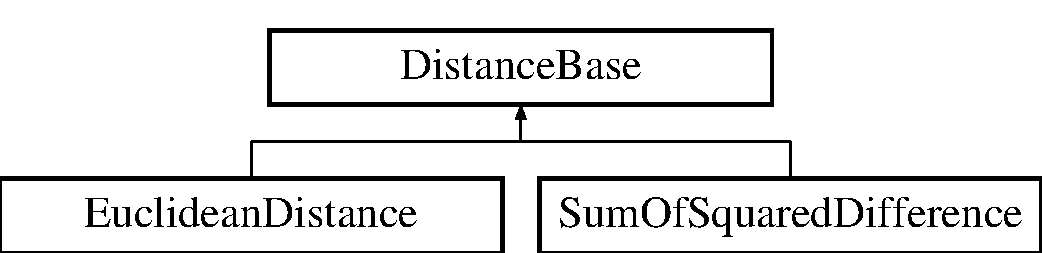
\includegraphics[height=2.000000cm]{class_distance_base}
\end{center}
\end{figure}
\subsection*{Public Member Functions}
\begin{DoxyCompactItemize}
\item 
virtual double \hyperlink{class_distance_base_aafc76227a800dd0827bedefded215646}{get\+Distance} (Mat image, Mat appearance)=0
\begin{DoxyCompactList}\small\item\em Gets the distance normalised between 0 and 1. \end{DoxyCompactList}\item 
double \hyperlink{class_distance_base_af22d9248a5ac76c62b7f0dbe5ee99251}{get\+Max\+Distance} ()
\begin{DoxyCompactList}\small\item\em Gets the highest distance value between the initial appearance and the intial frame. \end{DoxyCompactList}\end{DoxyCompactItemize}
\subsection*{Protected Member Functions}
\begin{DoxyCompactItemize}
\item 
double \hyperlink{class_distance_base_aa98d8e96cd683f814d9a8b6e5ad93836}{calculate\+S\+S\+D} (Mat image, Mat appearance)
\begin{DoxyCompactList}\small\item\em Both euclidean\+Distance and sum\+Of\+Squared\+Difference use a similar method to calculate the distance, so this is used to prevent repeared code. \end{DoxyCompactList}\end{DoxyCompactItemize}
\subsection*{Protected Attributes}
\begin{DoxyCompactItemize}
\item 
\hypertarget{class_distance_base_a29ed8af6966be2917dd4037bde9d8797}{}double {\bfseries max\+Distance}\label{class_distance_base_a29ed8af6966be2917dd4037bde9d8797}

\end{DoxyCompactItemize}


\subsection{Detailed Description}
This acts as and interface and holds the implementation common to Euclidean\+Distanace and \hyperlink{class_sum_of_squared_difference}{Sum\+Of\+Squared\+Difference}. 

\subsection{Member Function Documentation}
\hypertarget{class_distance_base_aa98d8e96cd683f814d9a8b6e5ad93836}{}\index{Distance\+Base@{Distance\+Base}!calculate\+S\+S\+D@{calculate\+S\+S\+D}}
\index{calculate\+S\+S\+D@{calculate\+S\+S\+D}!Distance\+Base@{Distance\+Base}}
\subsubsection[{calculate\+S\+S\+D}]{\setlength{\rightskip}{0pt plus 5cm}Distance\+Base\+::calculate\+S\+S\+D (
\begin{DoxyParamCaption}
\item[{Mat}]{image, }
\item[{Mat}]{appearance}
\end{DoxyParamCaption}
)\hspace{0.3cm}{\ttfamily [protected]}}\label{class_distance_base_aa98d8e96cd683f814d9a8b6e5ad93836}


Both euclidean\+Distance and sum\+Of\+Squared\+Difference use a similar method to calculate the distance, so this is used to prevent repeared code. 


\begin{DoxyParams}{Parameters}
{\em image} & \mbox{[}in\mbox{]} \\
\hline
{\em appearance} & \mbox{[}in\mbox{]} \\
\hline
\end{DoxyParams}
\begin{DoxyReturn}{Returns}
the distance between the image and the appearance 
\end{DoxyReturn}
\hypertarget{class_distance_base_aafc76227a800dd0827bedefded215646}{}\index{Distance\+Base@{Distance\+Base}!get\+Distance@{get\+Distance}}
\index{get\+Distance@{get\+Distance}!Distance\+Base@{Distance\+Base}}
\subsubsection[{get\+Distance}]{\setlength{\rightskip}{0pt plus 5cm}Distance\+Base\+::get\+Distance (
\begin{DoxyParamCaption}
\item[{Mat}]{image, }
\item[{Mat}]{appearance}
\end{DoxyParamCaption}
)\hspace{0.3cm}{\ttfamily [pure virtual]}}\label{class_distance_base_aafc76227a800dd0827bedefded215646}


Gets the distance normalised between 0 and 1. 


\begin{DoxyParams}{Parameters}
{\em image} & \mbox{[}in\mbox{]} \\
\hline
{\em appearance} & \mbox{[}in\mbox{]} \\
\hline
\end{DoxyParams}
\begin{DoxyReturn}{Returns}
the distance 
\end{DoxyReturn}


Implemented in \hyperlink{class_euclidean_distance_a1b3123ed61577c68d3c5fa1767950314}{Euclidean\+Distance}, and \hyperlink{class_sum_of_squared_difference_acd647d0817edf9cce383caa657ab46fa}{Sum\+Of\+Squared\+Difference}.

\hypertarget{class_distance_base_af22d9248a5ac76c62b7f0dbe5ee99251}{}\index{Distance\+Base@{Distance\+Base}!get\+Max\+Distance@{get\+Max\+Distance}}
\index{get\+Max\+Distance@{get\+Max\+Distance}!Distance\+Base@{Distance\+Base}}
\subsubsection[{get\+Max\+Distance}]{\setlength{\rightskip}{0pt plus 5cm}Distance\+Base\+::get\+Max\+Distance (
\begin{DoxyParamCaption}
{}
\end{DoxyParamCaption}
)}\label{class_distance_base_af22d9248a5ac76c62b7f0dbe5ee99251}


Gets the highest distance value between the initial appearance and the intial frame. 

\begin{DoxyReturn}{Returns}
the maximum distance 
\end{DoxyReturn}


The documentation for this class was generated from the following files\+:\begin{DoxyCompactItemize}
\item 
Distance\+Measures/distance\+Base.\+h\item 
Distance\+Measures/\hyperlink{distance_base_8cpp}{distance\+Base.\+cpp}\end{DoxyCompactItemize}

\hypertarget{class_euclidean_distance}{}\section{Euclidean\+Distance Class Reference}
\label{class_euclidean_distance}\index{Euclidean\+Distance@{Euclidean\+Distance}}


Used to calculate the Euclidean distance between two appearances.  




{\ttfamily \#include $<$euclidean\+Distance.\+h$>$}

Inheritance diagram for Euclidean\+Distance\+:\begin{figure}[H]
\begin{center}
\leavevmode
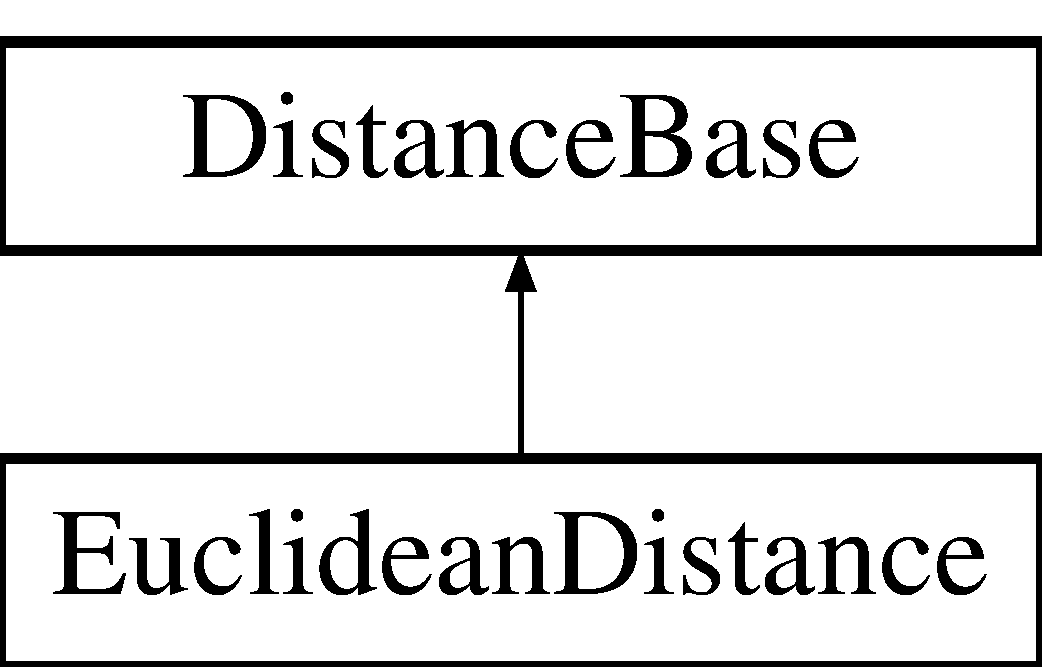
\includegraphics[height=2.000000cm]{class_euclidean_distance}
\end{center}
\end{figure}
\subsection*{Public Member Functions}
\begin{DoxyCompactItemize}
\item 
\hyperlink{class_euclidean_distance_a5e83b718959ef7c4b41d88b6b2f1cc97}{Euclidean\+Distance} (Mat frame, Mat appearance)
\begin{DoxyCompactList}\small\item\em Will set the max\+Distance the unnormalised euclidean distance should return. \end{DoxyCompactList}\item 
\hypertarget{class_euclidean_distance_a345c01bfb2649bb9c7f93eb04edf3c03}{}\hyperlink{class_euclidean_distance_a345c01bfb2649bb9c7f93eb04edf3c03}{Euclidean\+Distance} ()\label{class_euclidean_distance_a345c01bfb2649bb9c7f93eb04edf3c03}

\begin{DoxyCompactList}\small\item\em Used by the unit tests. \end{DoxyCompactList}\item 
double \hyperlink{class_euclidean_distance_a1b3123ed61577c68d3c5fa1767950314}{get\+Distance} (Mat image, Mat appearance)
\begin{DoxyCompactList}\small\item\em Gets the distance normalised between 0 and 1. \end{DoxyCompactList}\end{DoxyCompactItemize}
\subsection*{Additional Inherited Members}


\subsection{Detailed Description}
Used to calculate the Euclidean distance between two appearances. 

\subsection{Constructor \& Destructor Documentation}
\hypertarget{class_euclidean_distance_a5e83b718959ef7c4b41d88b6b2f1cc97}{}\index{Euclidean\+Distance@{Euclidean\+Distance}!Euclidean\+Distance@{Euclidean\+Distance}}
\index{Euclidean\+Distance@{Euclidean\+Distance}!Euclidean\+Distance@{Euclidean\+Distance}}
\subsubsection[{Euclidean\+Distance}]{\setlength{\rightskip}{0pt plus 5cm}Euclidean\+Distance\+::\+Euclidean\+Distance (
\begin{DoxyParamCaption}
\item[{Mat}]{frame, }
\item[{Mat}]{appearance}
\end{DoxyParamCaption}
)}\label{class_euclidean_distance_a5e83b718959ef7c4b41d88b6b2f1cc97}


Will set the max\+Distance the unnormalised euclidean distance should return. 


\begin{DoxyParams}{Parameters}
{\em frame} & \mbox{[}in\mbox{]} \+: The frame whch the appearance has been selected from \\
\hline
{\em appearance} & \mbox{[}in\mbox{]} \+: The appearance the user has selected \\
\hline
\end{DoxyParams}


\subsection{Member Function Documentation}
\hypertarget{class_euclidean_distance_a1b3123ed61577c68d3c5fa1767950314}{}\index{Euclidean\+Distance@{Euclidean\+Distance}!get\+Distance@{get\+Distance}}
\index{get\+Distance@{get\+Distance}!Euclidean\+Distance@{Euclidean\+Distance}}
\subsubsection[{get\+Distance}]{\setlength{\rightskip}{0pt plus 5cm}double Euclidean\+Distance\+::get\+Distance (
\begin{DoxyParamCaption}
\item[{Mat}]{image, }
\item[{Mat}]{appearance}
\end{DoxyParamCaption}
)\hspace{0.3cm}{\ttfamily [virtual]}}\label{class_euclidean_distance_a1b3123ed61577c68d3c5fa1767950314}


Gets the distance normalised between 0 and 1. 


\begin{DoxyParams}{Parameters}
{\em image} & \mbox{[}in\mbox{]} \\
\hline
{\em appearance} & \mbox{[}in\mbox{]} \\
\hline
\end{DoxyParams}
\begin{DoxyReturn}{Returns}
the distance 
\end{DoxyReturn}


Implements \hyperlink{class_distance_base_aafc76227a800dd0827bedefded215646}{Distance\+Base}.



The documentation for this class was generated from the following files\+:\begin{DoxyCompactItemize}
\item 
Distance\+Measures/\hyperlink{euclidean_distance_8h}{euclidean\+Distance.\+h}\item 
Distance\+Measures/\hyperlink{euclidean_distance_8cpp}{euclidean\+Distance.\+cpp}\end{DoxyCompactItemize}

\hypertarget{class_link_tracking_and_ui}{}\section{Link\+Tracking\+And\+Ui Class Reference}
\label{class_link_tracking_and_ui}\index{Link\+Tracking\+And\+Ui@{Link\+Tracking\+And\+Ui}}


Links the backend tracking code to the front end (U\+I) code.  




{\ttfamily \#include $<$link\+Tracking\+And\+Ui.\+h$>$}

Inheritance diagram for Link\+Tracking\+And\+Ui\+:\begin{figure}[H]
\begin{center}
\leavevmode
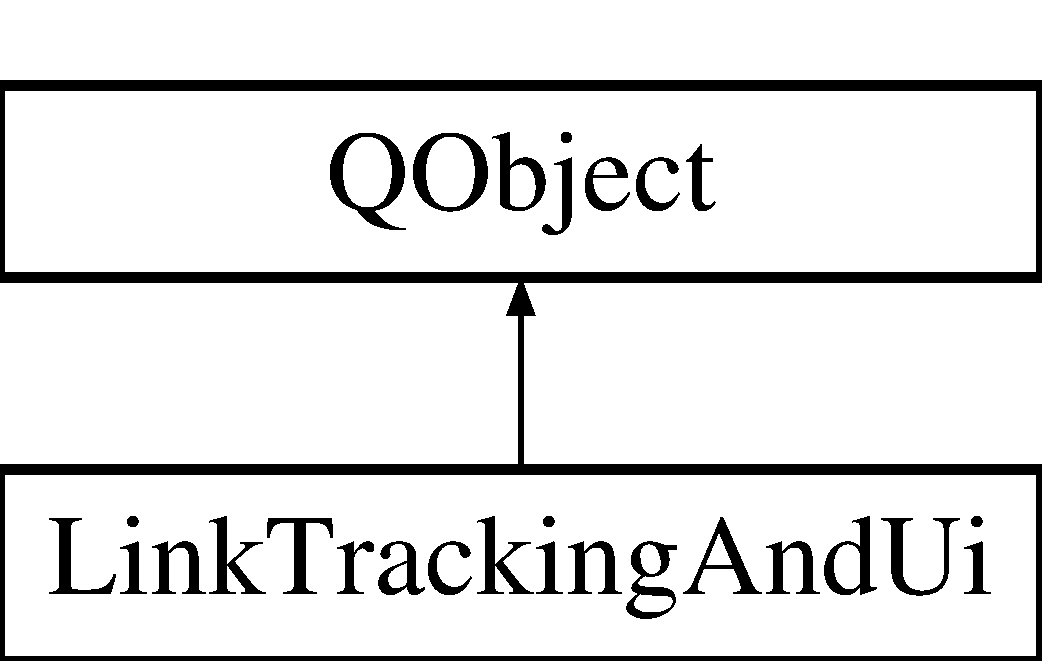
\includegraphics[height=2.000000cm]{class_link_tracking_and_ui}
\end{center}
\end{figure}
\subsection*{Public Member Functions}
\begin{DoxyCompactItemize}
\item 
\hyperlink{class_link_tracking_and_ui_a6f4f4209f002459ac29511c55d9b4780}{Link\+Tracking\+And\+Ui} (\hyperlink{class_qt_widget_image_display}{Qt\+Widget\+Image\+Display} $\ast$image\+Widget, \hyperlink{class_tracking_and_detection}{Tracking\+And\+Detection} $\ast$tracking\+And\+Detection)
\begin{DoxyCompactList}\small\item\em The tracking and detection is run in a different thread to the U\+I so this is used to allow data to be passed between the tracking\+And\+Detection object and the image\+Widget object. \end{DoxyCompactList}\end{DoxyCompactItemize}


\subsection{Detailed Description}
Links the backend tracking code to the front end (U\+I) code. 

\subsection{Constructor \& Destructor Documentation}
\hypertarget{class_link_tracking_and_ui_a6f4f4209f002459ac29511c55d9b4780}{}\index{Link\+Tracking\+And\+Ui@{Link\+Tracking\+And\+Ui}!Link\+Tracking\+And\+Ui@{Link\+Tracking\+And\+Ui}}
\index{Link\+Tracking\+And\+Ui@{Link\+Tracking\+And\+Ui}!Link\+Tracking\+And\+Ui@{Link\+Tracking\+And\+Ui}}
\subsubsection[{Link\+Tracking\+And\+Ui}]{\setlength{\rightskip}{0pt plus 5cm}Link\+Tracking\+And\+Ui\+::\+Link\+Tracking\+And\+Ui (
\begin{DoxyParamCaption}
\item[{{\bf Qt\+Widget\+Image\+Display} $\ast$}]{image\+Widget, }
\item[{{\bf Tracking\+And\+Detection} $\ast$}]{tracking\+And\+Detection}
\end{DoxyParamCaption}
)}\label{class_link_tracking_and_ui_a6f4f4209f002459ac29511c55d9b4780}


The tracking and detection is run in a different thread to the U\+I so this is used to allow data to be passed between the tracking\+And\+Detection object and the image\+Widget object. 


\begin{DoxyParams}{Parameters}
{\em image\+Widget} & \mbox{[}in\mbox{]} \\
\hline
{\em tracking\+And\+Detection} & \mbox{[}in\mbox{]} \\
\hline
\end{DoxyParams}


The documentation for this class was generated from the following files\+:\begin{DoxyCompactItemize}
\item 
\hyperlink{link_tracking_and_ui_8h}{link\+Tracking\+And\+Ui.\+h}\item 
\hyperlink{link_tracking_and_ui_8cpp}{link\+Tracking\+And\+Ui.\+cpp}\end{DoxyCompactItemize}

\hypertarget{struct_a_i_s___options_1_1_location}{}\section{A\+I\+S\+\_\+\+Options\+:\+:Location Struct Reference}
\label{struct_a_i_s___options_1_1_location}\index{A\+I\+S\+\_\+\+Options\+::\+Location@{A\+I\+S\+\_\+\+Options\+::\+Location}}
\subsection*{Public Attributes}
\begin{DoxyCompactItemize}
\item 
\hypertarget{struct_a_i_s___options_1_1_location_a924b78d8faca62b0f20d95033d4caf14}{}int {\bfseries x}\label{struct_a_i_s___options_1_1_location_a924b78d8faca62b0f20d95033d4caf14}

\item 
\hypertarget{struct_a_i_s___options_1_1_location_ae440db7ecbca694e7cd7bf38f6a643db}{}int {\bfseries y}\label{struct_a_i_s___options_1_1_location_ae440db7ecbca694e7cd7bf38f6a643db}

\item 
\hypertarget{struct_a_i_s___options_1_1_location_aa8912cf7ec3ecf0a0e60967ec7df125f}{}double {\bfseries scale\+X}\label{struct_a_i_s___options_1_1_location_aa8912cf7ec3ecf0a0e60967ec7df125f}

\item 
\hypertarget{struct_a_i_s___options_1_1_location_ab3d8de3e46148a2f12314e7813be90d4}{}double {\bfseries scale\+Y}\label{struct_a_i_s___options_1_1_location_ab3d8de3e46148a2f12314e7813be90d4}

\item 
\hypertarget{struct_a_i_s___options_1_1_location_a4c201c5c5889c22444a1bd47aaf927f3}{}int {\bfseries rotation}\label{struct_a_i_s___options_1_1_location_a4c201c5c5889c22444a1bd47aaf927f3}

\end{DoxyCompactItemize}


The documentation for this struct was generated from the following file\+:\begin{DoxyCompactItemize}
\item 
\hyperlink{options_8h}{options.\+h}\end{DoxyCompactItemize}

\hypertarget{class_main_window}{}\section{Main\+Window Class Reference}
\label{class_main_window}\index{Main\+Window@{Main\+Window}}


The main U\+I window.  




{\ttfamily \#include $<$mainwindow.\+h$>$}

Inheritance diagram for Main\+Window\+:\begin{figure}[H]
\begin{center}
\leavevmode
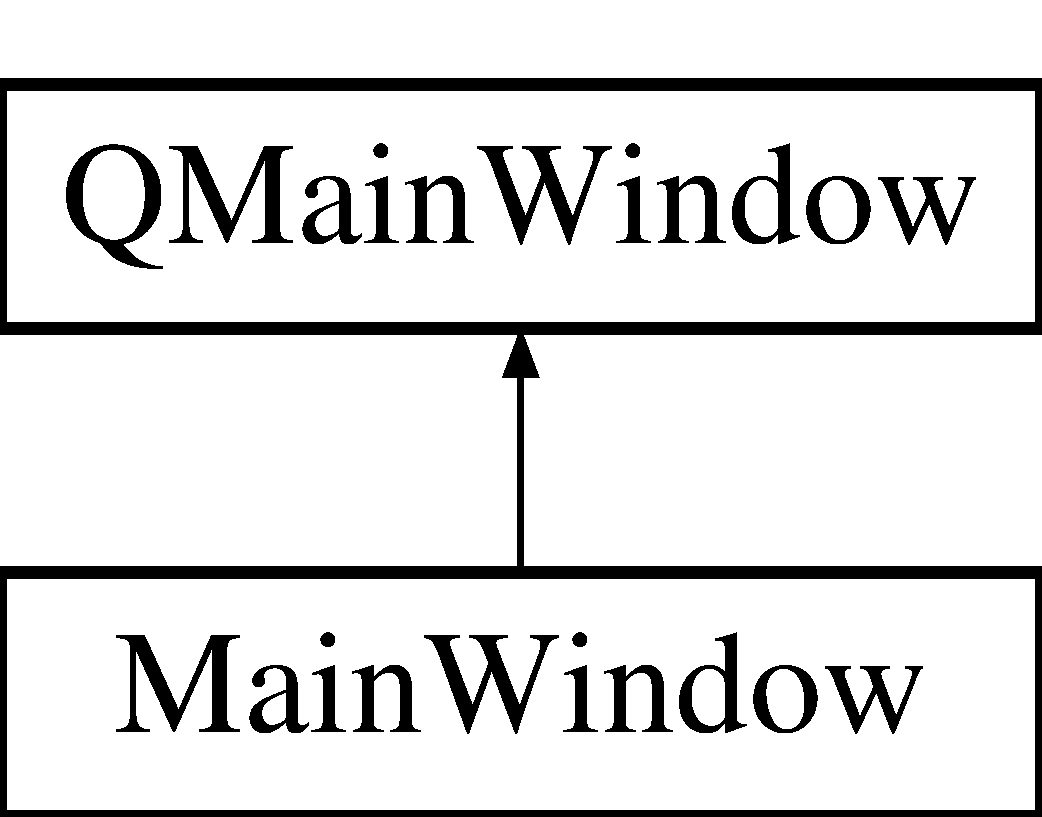
\includegraphics[height=2.000000cm]{class_main_window}
\end{center}
\end{figure}
\subsection*{Public Member Functions}
\begin{DoxyCompactItemize}
\item 
\hypertarget{class_main_window_a8b244be8b7b7db1b08de2a2acb9409db}{}{\bfseries Main\+Window} (Q\+Widget $\ast$parent=0)\label{class_main_window_a8b244be8b7b7db1b08de2a2acb9409db}

\item 
\hyperlink{class_qt_widget_image_display}{Qt\+Widget\+Image\+Display} $\ast$ \hyperlink{class_main_window_afaa035415cb58eb48bf7cc4d9a07784b}{get\+Image\+Widget} ()
\end{DoxyCompactItemize}


\subsection{Detailed Description}
The main U\+I window. 

\subsection{Member Function Documentation}
\hypertarget{class_main_window_afaa035415cb58eb48bf7cc4d9a07784b}{}\index{Main\+Window@{Main\+Window}!get\+Image\+Widget@{get\+Image\+Widget}}
\index{get\+Image\+Widget@{get\+Image\+Widget}!Main\+Window@{Main\+Window}}
\subsubsection[{get\+Image\+Widget}]{\setlength{\rightskip}{0pt plus 5cm}Main\+Window\+::get\+Image\+Widget (
\begin{DoxyParamCaption}
{}
\end{DoxyParamCaption}
)}\label{class_main_window_afaa035415cb58eb48bf7cc4d9a07784b}
\begin{DoxyReturn}{Returns}
gets a pointer to the \hyperlink{class_qt_widget_image_display}{Qt\+Widget\+Image\+Display} 
\end{DoxyReturn}


The documentation for this class was generated from the following files\+:\begin{DoxyCompactItemize}
\item 
U\+I/\hyperlink{mainwindow_8h}{mainwindow.\+h}\item 
U\+I/\hyperlink{mainwindow_8cpp}{mainwindow.\+cpp}\end{DoxyCompactItemize}

\hypertarget{class_network}{}\section{Network Class Reference}
\label{class_network}\index{Network@{Network}}


Holds the network of A\+R\+Bs. Handles the adding and removing of A\+R\+Bs.  




{\ttfamily \#include $<$network.\+h$>$}

\subsection*{Public Member Functions}
\begin{DoxyCompactItemize}
\item 
\hyperlink{class_network_abf40cbcbed14ec61e7a6d2b8e1dc6a1a}{Network} (Mat initial\+Apperance, \hyperlink{struct_a_i_s___options_1_1_location}{Location} current\+Location, \hyperlink{class_distance_base}{Distance\+Base} $\ast$distance\+Measure, double object\+Threshold, double stimulation\+Threshold)
\begin{DoxyCompactList}\small\item\em Constructor for the \hyperlink{class_network}{Network}. \end{DoxyCompactList}\item 
\hyperlink{struct_a_i_s___options_1_1_location}{Location} \hyperlink{class_network_a13011652e7fb84154942625ad3eb66c8}{add\+Appearance} (Mat appearance, \hyperlink{struct_a_i_s___options_1_1_location}{Location} current\+Location)
\begin{DoxyCompactList}\small\item\em Finds the closest \hyperlink{class_a_r_b}{A\+R\+B} and if the distance is below the S\+T\+I\+M\+U\+L\+A\+T\+I\+O\+N\+\_\+\+T\+H\+R\+E\+S\+H\+O\+L\+D increases the resource of that \hyperlink{class_a_r_b}{A\+R\+B}. If the distance is not below the S\+T\+I\+M\+U\+L\+A\+T\+I\+O\+N\+\_\+\+T\+H\+R\+E\+S\+H\+O\+L\+D then creates a new \hyperlink{class_a_r_b}{A\+R\+B}. The \hyperlink{class_a_r_b}{A\+R\+B} is linked to the previous known \hyperlink{class_a_r_b}{A\+R\+B}. \end{DoxyCompactList}\item 
vector$<$ Mat $>$ \hyperlink{class_network_afcd78f9225ca2f2f92d1b1db870ffb65}{get\+A\+R\+Bs\+With\+Above\+Average\+R\+L} ()
\begin{DoxyCompactList}\small\item\em Gets the nodes that performs the inital search for the object within a video frame. \end{DoxyCompactList}\item 
vector$<$ Mat $>$ \hyperlink{class_network_a976fa4622de1dc318bd5af89ebd17ac6}{get\+All\+Appearances} ()
\item 
vector$<$ Mat $>$ \hyperlink{class_network_afc66817b2698ce006c508ee8842375b9}{get\+Last\+And\+Highest\+A\+R\+Bs} ()
\item 
\hyperlink{struct_a_i_s___options_1_1_location}{Location} \hyperlink{class_network_a0b0624d5507f67a840e96821b81e472f}{get\+Predicted\+Location} ()
\item 
int \hyperlink{class_network_aa711dad35933517182c6cbe32b1997b2}{get\+Number\+Of\+A\+R\+Bs} ()
\item 
vector$<$ \hyperlink{class_a_r_b}{A\+R\+B} $\ast$ $>$ \hyperlink{class_network_a833cd5788cfe15365bfc67c8db8e8cb6}{get\+A\+R\+Bs} ()
\item 
void \hyperlink{class_network_a652c03f659bba278fd7b5fd345c61f5d}{set\+Use\+Predicted\+Location} (bool use\+Predicted\+Location)
\item 
void \hyperlink{class_network_a4c9a48c5a3b025d44e3febbedac3bfe3}{set\+Obejct\+Threshold} (double object\+Threshold)
\item 
void \hyperlink{class_network_a91de437f331fdac84919c3606c1b6f83}{set\+Stimulation\+Threshold} (double stimulation\+Threshold)
\end{DoxyCompactItemize}


\subsection{Detailed Description}
Holds the network of A\+R\+Bs. Handles the adding and removing of A\+R\+Bs. 

\subsection{Constructor \& Destructor Documentation}
\hypertarget{class_network_abf40cbcbed14ec61e7a6d2b8e1dc6a1a}{}\index{Network@{Network}!Network@{Network}}
\index{Network@{Network}!Network@{Network}}
\subsubsection[{Network}]{\setlength{\rightskip}{0pt plus 5cm}Network\+::\+Network (
\begin{DoxyParamCaption}
\item[{Mat}]{initial\+Apperance, }
\item[{{\bf Location}}]{current\+Location, }
\item[{{\bf Distance\+Base} $\ast$}]{distance\+Measure, }
\item[{double}]{object\+Threshold, }
\item[{double}]{stimulation\+Threshold}
\end{DoxyParamCaption}
)}\label{class_network_abf40cbcbed14ec61e7a6d2b8e1dc6a1a}


Constructor for the \hyperlink{class_network}{Network}. 


\begin{DoxyParams}{Parameters}
{\em initial\+Apperance} & \mbox{[}in\mbox{]} \+: The appearance that the user has selected. \\
\hline
{\em current\+Location} & \mbox{[}in\mbox{]} \+: The initial location. \\
\hline
\end{DoxyParams}


\subsection{Member Function Documentation}
\hypertarget{class_network_a13011652e7fb84154942625ad3eb66c8}{}\index{Network@{Network}!add\+Appearance@{add\+Appearance}}
\index{add\+Appearance@{add\+Appearance}!Network@{Network}}
\subsubsection[{add\+Appearance}]{\setlength{\rightskip}{0pt plus 5cm}Network\+::add\+Appearance (
\begin{DoxyParamCaption}
\item[{Mat}]{appearance, }
\item[{{\bf Location}}]{current\+Location}
\end{DoxyParamCaption}
)}\label{class_network_a13011652e7fb84154942625ad3eb66c8}


Finds the closest \hyperlink{class_a_r_b}{A\+R\+B} and if the distance is below the S\+T\+I\+M\+U\+L\+A\+T\+I\+O\+N\+\_\+\+T\+H\+R\+E\+S\+H\+O\+L\+D increases the resource of that \hyperlink{class_a_r_b}{A\+R\+B}. If the distance is not below the S\+T\+I\+M\+U\+L\+A\+T\+I\+O\+N\+\_\+\+T\+H\+R\+E\+S\+H\+O\+L\+D then creates a new \hyperlink{class_a_r_b}{A\+R\+B}. The \hyperlink{class_a_r_b}{A\+R\+B} is linked to the previous known \hyperlink{class_a_r_b}{A\+R\+B}. 


\begin{DoxyParams}{Parameters}
{\em appearance} & \mbox{[}in\mbox{]} \+: The appearance the network is being exposed to \\
\hline
{\em current\+Location} & \mbox{[}in\mbox{]} \+: The location the appearance is at \\
\hline
\end{DoxyParams}
\hypertarget{class_network_a976fa4622de1dc318bd5af89ebd17ac6}{}\index{Network@{Network}!get\+All\+Appearances@{get\+All\+Appearances}}
\index{get\+All\+Appearances@{get\+All\+Appearances}!Network@{Network}}
\subsubsection[{get\+All\+Appearances}]{\setlength{\rightskip}{0pt plus 5cm}Network\+::get\+All\+Appearances (
\begin{DoxyParamCaption}
{}
\end{DoxyParamCaption}
)}\label{class_network_a976fa4622de1dc318bd5af89ebd17ac6}
\begin{DoxyReturn}{Returns}
A list of all appearances in the network 
\end{DoxyReturn}
\hypertarget{class_network_a833cd5788cfe15365bfc67c8db8e8cb6}{}\index{Network@{Network}!get\+A\+R\+Bs@{get\+A\+R\+Bs}}
\index{get\+A\+R\+Bs@{get\+A\+R\+Bs}!Network@{Network}}
\subsubsection[{get\+A\+R\+Bs}]{\setlength{\rightskip}{0pt plus 5cm}Network\+::get\+A\+R\+Bs (
\begin{DoxyParamCaption}
{}
\end{DoxyParamCaption}
)}\label{class_network_a833cd5788cfe15365bfc67c8db8e8cb6}
\begin{DoxyReturn}{Returns}
A list of all A\+R\+Bs in the network 
\end{DoxyReturn}
\hypertarget{class_network_afcd78f9225ca2f2f92d1b1db870ffb65}{}\index{Network@{Network}!get\+A\+R\+Bs\+With\+Above\+Average\+R\+L@{get\+A\+R\+Bs\+With\+Above\+Average\+R\+L}}
\index{get\+A\+R\+Bs\+With\+Above\+Average\+R\+L@{get\+A\+R\+Bs\+With\+Above\+Average\+R\+L}!Network@{Network}}
\subsubsection[{get\+A\+R\+Bs\+With\+Above\+Average\+R\+L}]{\setlength{\rightskip}{0pt plus 5cm}Network\+::get\+A\+R\+Bs\+With\+Above\+Average\+R\+L (
\begin{DoxyParamCaption}
{}
\end{DoxyParamCaption}
)}\label{class_network_afcd78f9225ca2f2f92d1b1db870ffb65}


Gets the nodes that performs the inital search for the object within a video frame. 

\begin{DoxyReturn}{Returns}
The previous appearance and the most stimulated appearance 
\end{DoxyReturn}
\hypertarget{class_network_afc66817b2698ce006c508ee8842375b9}{}\index{Network@{Network}!get\+Last\+And\+Highest\+A\+R\+Bs@{get\+Last\+And\+Highest\+A\+R\+Bs}}
\index{get\+Last\+And\+Highest\+A\+R\+Bs@{get\+Last\+And\+Highest\+A\+R\+Bs}!Network@{Network}}
\subsubsection[{get\+Last\+And\+Highest\+A\+R\+Bs}]{\setlength{\rightskip}{0pt plus 5cm}Network\+::get\+Last\+And\+Highest\+A\+R\+Bs (
\begin{DoxyParamCaption}
{}
\end{DoxyParamCaption}
)}\label{class_network_afc66817b2698ce006c508ee8842375b9}
\begin{DoxyReturn}{Returns}
The last \hyperlink{class_a_r_b}{A\+R\+B} to be used and the \hyperlink{class_a_r_b}{A\+R\+B} which has the highest resource level 
\end{DoxyReturn}
\hypertarget{class_network_aa711dad35933517182c6cbe32b1997b2}{}\index{Network@{Network}!get\+Number\+Of\+A\+R\+Bs@{get\+Number\+Of\+A\+R\+Bs}}
\index{get\+Number\+Of\+A\+R\+Bs@{get\+Number\+Of\+A\+R\+Bs}!Network@{Network}}
\subsubsection[{get\+Number\+Of\+A\+R\+Bs}]{\setlength{\rightskip}{0pt plus 5cm}Network\+::get\+Number\+Of\+A\+R\+Bs (
\begin{DoxyParamCaption}
{}
\end{DoxyParamCaption}
)}\label{class_network_aa711dad35933517182c6cbe32b1997b2}
\begin{DoxyReturn}{Returns}
The number of A\+R\+Bs 
\end{DoxyReturn}
\hypertarget{class_network_a0b0624d5507f67a840e96821b81e472f}{}\index{Network@{Network}!get\+Predicted\+Location@{get\+Predicted\+Location}}
\index{get\+Predicted\+Location@{get\+Predicted\+Location}!Network@{Network}}
\subsubsection[{get\+Predicted\+Location}]{\setlength{\rightskip}{0pt plus 5cm}Network\+::get\+Predicted\+Location (
\begin{DoxyParamCaption}
{}
\end{DoxyParamCaption}
)}\label{class_network_a0b0624d5507f67a840e96821b81e472f}
\begin{DoxyReturn}{Returns}
The objects predicted location 
\end{DoxyReturn}
\hypertarget{class_network_a4c9a48c5a3b025d44e3febbedac3bfe3}{}\index{Network@{Network}!set\+Obejct\+Threshold@{set\+Obejct\+Threshold}}
\index{set\+Obejct\+Threshold@{set\+Obejct\+Threshold}!Network@{Network}}
\subsubsection[{set\+Obejct\+Threshold}]{\setlength{\rightskip}{0pt plus 5cm}Network\+::set\+Obejct\+Threshold (
\begin{DoxyParamCaption}
\item[{double}]{object\+Threshold}
\end{DoxyParamCaption}
)}\label{class_network_a4c9a48c5a3b025d44e3febbedac3bfe3}

\begin{DoxyParams}{Parameters}
{\em object\+Threshold} & \\
\hline
\end{DoxyParams}
\hypertarget{class_network_a91de437f331fdac84919c3606c1b6f83}{}\index{Network@{Network}!set\+Stimulation\+Threshold@{set\+Stimulation\+Threshold}}
\index{set\+Stimulation\+Threshold@{set\+Stimulation\+Threshold}!Network@{Network}}
\subsubsection[{set\+Stimulation\+Threshold}]{\setlength{\rightskip}{0pt plus 5cm}Network\+::set\+Stimulation\+Threshold (
\begin{DoxyParamCaption}
\item[{double}]{stimulation\+Threshold}
\end{DoxyParamCaption}
)}\label{class_network_a91de437f331fdac84919c3606c1b6f83}

\begin{DoxyParams}{Parameters}
{\em stimulation\+Threshold} & \\
\hline
\end{DoxyParams}
\hypertarget{class_network_a652c03f659bba278fd7b5fd345c61f5d}{}\index{Network@{Network}!set\+Use\+Predicted\+Location@{set\+Use\+Predicted\+Location}}
\index{set\+Use\+Predicted\+Location@{set\+Use\+Predicted\+Location}!Network@{Network}}
\subsubsection[{set\+Use\+Predicted\+Location}]{\setlength{\rightskip}{0pt plus 5cm}Network\+::set\+Use\+Predicted\+Location (
\begin{DoxyParamCaption}
\item[{bool}]{use\+Predicted\+Location}
\end{DoxyParamCaption}
)}\label{class_network_a652c03f659bba278fd7b5fd345c61f5d}

\begin{DoxyParams}{Parameters}
{\em use\+Predicted\+Location} & \mbox{[}in\mbox{]} \\
\hline
\end{DoxyParams}


The documentation for this class was generated from the following files\+:\begin{DoxyCompactItemize}
\item 
A\+I\+S/\hyperlink{network_8h}{network.\+h}\item 
A\+I\+S/\hyperlink{network_8cpp}{network.\+cpp}\end{DoxyCompactItemize}

\hypertarget{class_output_data}{}\section{Output\+Data Class Reference}
\label{class_output_data}\index{Output\+Data@{Output\+Data}}


Allows the A\+I\+N to be saved to file.  




{\ttfamily \#include $<$output\+Data.\+h$>$}

\subsection*{Public Member Functions}
\begin{DoxyCompactItemize}
\item 
void \hyperlink{class_output_data_aa233ec3bd0c4b9f381ba8ccb46f21443}{write\+Num\+Of\+A\+R\+Bs} (string file\+Name, vector$<$ int $>$ num\+A\+R\+Bs\+List)
\begin{DoxyCompactList}\small\item\em Writes out a file listing the number of A\+R\+Bs the network has contained. \end{DoxyCompactList}\item 
void \hyperlink{class_output_data_acccb676f62c27d703a7aae83333ab5ca}{save\+Network} (string directory\+Name, \hyperlink{class_network}{Network} $\ast$network)
\begin{DoxyCompactList}\small\item\em Saves the appearances to image files and creates a text file containing information about how the appearances are joined in the network. \end{DoxyCompactList}\item 
void \hyperlink{class_output_data_a6928c41ff82d541ac1eecef838358414}{write\+Frame\+Rates} (string file\+Name, vector$<$ double $>$ frame\+Rates)
\begin{DoxyCompactList}\small\item\em Writes the list of frame rates to file. \end{DoxyCompactList}\end{DoxyCompactItemize}


\subsection{Detailed Description}
Allows the A\+I\+N to be saved to file. 

\subsection{Member Function Documentation}
\hypertarget{class_output_data_acccb676f62c27d703a7aae83333ab5ca}{}\index{Output\+Data@{Output\+Data}!save\+Network@{save\+Network}}
\index{save\+Network@{save\+Network}!Output\+Data@{Output\+Data}}
\subsubsection[{save\+Network}]{\setlength{\rightskip}{0pt plus 5cm}Output\+Data\+::save\+Network (
\begin{DoxyParamCaption}
\item[{string}]{directory\+Name, }
\item[{{\bf Network} $\ast$}]{network}
\end{DoxyParamCaption}
)}\label{class_output_data_acccb676f62c27d703a7aae83333ab5ca}


Saves the appearances to image files and creates a text file containing information about how the appearances are joined in the network. 


\begin{DoxyParams}{Parameters}
{\em directory\+Name} & \mbox{[}in\mbox{]} \\
\hline
{\em network} & \mbox{[}in\mbox{]} \\
\hline
\end{DoxyParams}
\hypertarget{class_output_data_a6928c41ff82d541ac1eecef838358414}{}\index{Output\+Data@{Output\+Data}!write\+Frame\+Rates@{write\+Frame\+Rates}}
\index{write\+Frame\+Rates@{write\+Frame\+Rates}!Output\+Data@{Output\+Data}}
\subsubsection[{write\+Frame\+Rates}]{\setlength{\rightskip}{0pt plus 5cm}Output\+Data\+::write\+Frame\+Rates (
\begin{DoxyParamCaption}
\item[{string}]{file\+Name, }
\item[{vector$<$ double $>$}]{frame\+Rates}
\end{DoxyParamCaption}
)}\label{class_output_data_a6928c41ff82d541ac1eecef838358414}


Writes the list of frame rates to file. 


\begin{DoxyParams}{Parameters}
{\em file\+Name} & \mbox{[}in\mbox{]} \\
\hline
{\em frame\+Rates} & \mbox{[}in\mbox{]} \\
\hline
\end{DoxyParams}
\hypertarget{class_output_data_aa233ec3bd0c4b9f381ba8ccb46f21443}{}\index{Output\+Data@{Output\+Data}!write\+Num\+Of\+A\+R\+Bs@{write\+Num\+Of\+A\+R\+Bs}}
\index{write\+Num\+Of\+A\+R\+Bs@{write\+Num\+Of\+A\+R\+Bs}!Output\+Data@{Output\+Data}}
\subsubsection[{write\+Num\+Of\+A\+R\+Bs}]{\setlength{\rightskip}{0pt plus 5cm}Output\+Data\+::write\+Num\+Of\+A\+R\+Bs (
\begin{DoxyParamCaption}
\item[{string}]{file\+Name, }
\item[{vector$<$ int $>$}]{num\+A\+R\+Bs\+List}
\end{DoxyParamCaption}
)}\label{class_output_data_aa233ec3bd0c4b9f381ba8ccb46f21443}


Writes out a file listing the number of A\+R\+Bs the network has contained. 


\begin{DoxyParams}{Parameters}
{\em file\+Name} & \mbox{[}in\mbox{]} \+: File path name to save the data to. \\
\hline
{\em num\+A\+R\+Bs\+List} & \mbox{[}in\mbox{]} \\
\hline
\end{DoxyParams}


The documentation for this class was generated from the following files\+:\begin{DoxyCompactItemize}
\item 
U\+I/output\+Data.\+h\item 
U\+I/\hyperlink{output_data_8cpp}{output\+Data.\+cpp}\end{DoxyCompactItemize}

\hypertarget{class_qt_widget_image_display}{}\section{Qt\+Widget\+Image\+Display Class Reference}
\label{class_qt_widget_image_display}\index{Qt\+Widget\+Image\+Display@{Qt\+Widget\+Image\+Display}}


Allows the video to be displayed and shows the position of the object being tracked.  




{\ttfamily \#include $<$qt\+Widget\+Image\+Display.\+h$>$}

Inheritance diagram for Qt\+Widget\+Image\+Display\+:\begin{figure}[H]
\begin{center}
\leavevmode
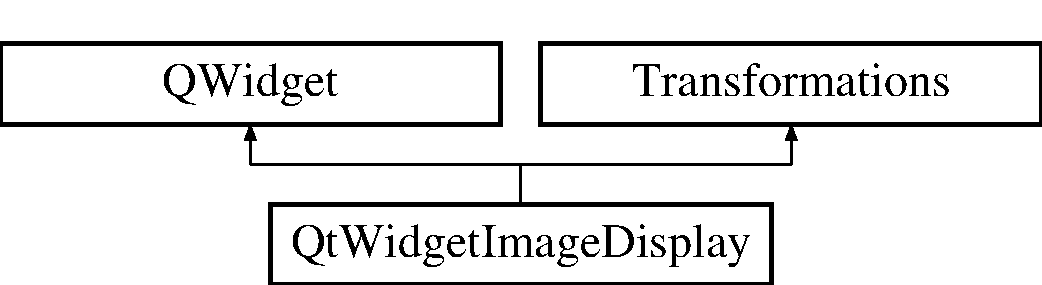
\includegraphics[height=2.000000cm]{class_qt_widget_image_display}
\end{center}
\end{figure}
\subsection*{Public Slots}
\begin{DoxyCompactItemize}
\item 
\hypertarget{class_qt_widget_image_display_aa65978984820243b551d99592342e8bc}{}void \hyperlink{class_qt_widget_image_display_aa65978984820243b551d99592342e8bc}{print\+Number\+Arbs\+In\+Network} ()\label{class_qt_widget_image_display_aa65978984820243b551d99592342e8bc}

\begin{DoxyCompactList}\small\item\em Asks the user for the file that the list of the number of A\+R\+Bs should be written to. \end{DoxyCompactList}\item 
\hypertarget{class_qt_widget_image_display_af1ec2373cfac14c17d4be8ea014aac7a}{}void \hyperlink{class_qt_widget_image_display_af1ec2373cfac14c17d4be8ea014aac7a}{save\+Network} ()\label{class_qt_widget_image_display_af1ec2373cfac14c17d4be8ea014aac7a}

\begin{DoxyCompactList}\small\item\em Asks the user for a directory to save the appearances in the network to. \end{DoxyCompactList}\item 
void \hyperlink{class_qt_widget_image_display_af57a98200b443711d226b079fa3a886a}{set\+Network\+To\+Save\+Network} (\hyperlink{class_network}{Network} $\ast$)
\begin{DoxyCompactList}\small\item\em The request for a copy of the \hyperlink{class_network}{Network} gets passed to here. \end{DoxyCompactList}\item 
\hypertarget{class_qt_widget_image_display_a5730944e528e82ec7bbe6ef71fd02e6b}{}void \hyperlink{class_qt_widget_image_display_a5730944e528e82ec7bbe6ef71fd02e6b}{get\+Video\+File\+Config} ()\label{class_qt_widget_image_display_a5730944e528e82ec7bbe6ef71fd02e6b}

\begin{DoxyCompactList}\small\item\em Allows the user to select the video configuration file that should be used. \end{DoxyCompactList}\item 
void \hyperlink{class_qt_widget_image_display_a67a3b1543b70d23c30c73b571a778cf2}{display\+Mat} (uchar $\ast$data, int cols, int rows)
\begin{DoxyCompactList}\small\item\em Shows the current video frame. \end{DoxyCompactList}\item 
void \hyperlink{class_qt_widget_image_display_a2f224c2a74780308829f77f915f82af5}{set\+Tracking\+Position} (int x, int y, int rotation, int width, int height)
\begin{DoxyCompactList}\small\item\em Sets the current position of the object being track, so that the box can be drawn. \end{DoxyCompactList}\item 
void \hyperlink{class_qt_widget_image_display_ad0e8669aaa03e5d49a9e9d63ee76655b}{set\+Num\+A\+R\+Bs} (int num\+A\+R\+Bs)
\begin{DoxyCompactList}\small\item\em Sets the number of A\+R\+Bs so that it can be displayed to the user. \end{DoxyCompactList}\end{DoxyCompactItemize}
\subsection*{Signals}
\begin{DoxyCompactItemize}
\item 
void \hyperlink{class_qt_widget_image_display_ae8d9428c993c2963636527fe6a5de437}{set\+Stimulation\+Threshold} (double stimulation\+Threshold)
\item 
void \hyperlink{class_qt_widget_image_display_a2458d0c43ad30f76425378d1af12c28c}{set\+Object\+Threshold} (double object\+Threshold)
\item 
void \hyperlink{class_qt_widget_image_display_aa45cd7ccb44eed2ffe8906bb638bbff8}{set\+Initial\+Tracking\+Postion} (int x, int y, int width, int height)
\begin{DoxyCompactList}\small\item\em Sets the initial position of the object. \end{DoxyCompactList}\item 
void \hyperlink{class_qt_widget_image_display_a4a319442190375dc4c6292cfdf0eb5d5}{set\+State} (Program\+State state)
\begin{DoxyCompactList}\small\item\em Sets if an obejct is being tracked or selected. \end{DoxyCompactList}\item 
void \hyperlink{class_qt_widget_image_display_a40b886057dfcebf207c50deb7a01ad76}{set\+Video\+Type} (Video\+Input\+Type input\+Type)
\item 
void \hyperlink{class_qt_widget_image_display_a7c6789b7f9e7abfa3fb514084fd45811}{set\+Video\+File\+Config\+File\+Path} (string file\+Path\+Name)
\item 
void \hyperlink{class_qt_widget_image_display_aad205e732e07afc1928cb4a4a58c5b97}{set\+Use\+Rotation} (bool use\+Rotation)
\item 
void \hyperlink{class_qt_widget_image_display_a2dabda43142dffe1416d3296087b2a3f}{set\+Use\+Scale} (bool use\+Scale)
\item 
void \hyperlink{class_qt_widget_image_display_a0eea72b2c4ce840d49e9d46502ae81b0}{set\+Use\+Predicted\+Location} (bool use\+Predicted\+Location)
\item 
void \hyperlink{class_qt_widget_image_display_ae99fa698ae5da37da20cd94192a7b0db}{set\+Distance\+Measure} (Distance\+Measure\+Type distance\+Measure\+Type)
\item 
\hypertarget{class_qt_widget_image_display_a6adb17100e4abae17a7e9074b7531e8e}{}void {\bfseries set\+Which\+A\+R\+Bs\+To\+Search\+With} (A\+R\+Bs\+To\+Search\+With which\+A\+R\+Bs\+To\+Search\+With)\label{class_qt_widget_image_display_a6adb17100e4abae17a7e9074b7531e8e}

\item 
\hypertarget{class_qt_widget_image_display_aaaf8f08ea03050bbee5aea48c3161e9f}{}void \hyperlink{class_qt_widget_image_display_aaaf8f08ea03050bbee5aea48c3161e9f}{get\+Network} ()\label{class_qt_widget_image_display_aaaf8f08ea03050bbee5aea48c3161e9f}

\begin{DoxyCompactList}\small\item\em A request for a copy of the network to be emited to this class. \end{DoxyCompactList}\end{DoxyCompactItemize}
\subsection*{Public Member Functions}
\begin{DoxyCompactItemize}
\item 
\hyperlink{class_qt_widget_image_display_a9ea3610dc3cae789d500b4f53cdb56b2}{Qt\+Widget\+Image\+Display} (Q\+Widget $\ast$parent=0)
\begin{DoxyCompactList}\small\item\em Calls parent constuctor and sets default variables. \end{DoxyCompactList}\item 
void \hyperlink{class_qt_widget_image_display_a26454c4394b3ae3bc9cb430f1107b27f}{which\+A\+R\+Bs\+To\+Search\+With\+Changed} (A\+R\+Bs\+To\+Search\+With which\+A\+R\+Bs\+To\+Search\+With)
\item 
void \hyperlink{class_qt_widget_image_display_ad8ff14b5736c02451e9671049377f804}{use\+Predicted\+Location\+Changed} (bool use\+Predicted\+Location)
\item 
void \hyperlink{class_qt_widget_image_display_a0ffc0b84135973ba32c75e2b42d9bb14}{distance\+Measure\+Changed} (Distance\+Measure\+Type distance\+Measure\+Type)
\item 
void \hyperlink{class_qt_widget_image_display_ab17105b0117339be323f990ff8089045}{use\+Rotation\+Changed} (bool use\+Rotation)
\item 
void \hyperlink{class_qt_widget_image_display_af598a9cee6959fcac05e8574bb2829ef}{use\+Scale\+Changed} (bool use\+Scale)
\item 
void \hyperlink{class_qt_widget_image_display_ab8581f2118716a98efda55054ab8b38c}{video\+Input\+Changed} (Video\+Input\+Type video\+Input\+Type)
\item 
void \hyperlink{class_qt_widget_image_display_a25b3298891cc5f2c085eadee653bb997}{stimulation\+Threshold\+Changed} (double stimulation\+Threshold)
\item 
void \hyperlink{class_qt_widget_image_display_a2fa5da388332212c0eff72bdc6ce0131}{object\+Threshold\+Changed} (double object\+Threshold)
\end{DoxyCompactItemize}
\subsection*{Protected Member Functions}
\begin{DoxyCompactItemize}
\item 
\hypertarget{class_qt_widget_image_display_a04130803d15b2efd86e7dc7b943d6508}{}void {\bfseries paint\+Event} (Q\+Paint\+Event $\ast$)\label{class_qt_widget_image_display_a04130803d15b2efd86e7dc7b943d6508}

\item 
void \hyperlink{class_qt_widget_image_display_a6235f02715be56b1d0c79a0162b3b3f5}{mouse\+Press\+Event} (Q\+Mouse\+Event $\ast$event)
\begin{DoxyCompactList}\small\item\em Allows the user to select the object they wish to track. \end{DoxyCompactList}\item 
void \hyperlink{class_qt_widget_image_display_ac299992cba352e07584839bb5e407cae}{mouse\+Move\+Event} (Q\+Mouse\+Event $\ast$event)
\begin{DoxyCompactList}\small\item\em Allows the user to select the object they wish to track. \end{DoxyCompactList}\item 
void \hyperlink{class_qt_widget_image_display_a1436ddfbe1ea7b4f2eb58552d50d077e}{mouse\+Release\+Event} (Q\+Mouse\+Event $\ast$event)
\begin{DoxyCompactList}\small\item\em Allows the user to select the object they wish to track. \end{DoxyCompactList}\end{DoxyCompactItemize}
\subsection*{Protected Attributes}
\begin{DoxyCompactItemize}
\item 
\hypertarget{class_qt_widget_image_display_a2d153ae169f34e0cfa9d8b491e6ef579}{}Q\+Image {\bfseries \+\_\+qimage}\label{class_qt_widget_image_display_a2d153ae169f34e0cfa9d8b491e6ef579}

\end{DoxyCompactItemize}


\subsection{Detailed Description}
Allows the video to be displayed and shows the position of the object being tracked. 

\subsection{Constructor \& Destructor Documentation}
\hypertarget{class_qt_widget_image_display_a9ea3610dc3cae789d500b4f53cdb56b2}{}\index{Qt\+Widget\+Image\+Display@{Qt\+Widget\+Image\+Display}!Qt\+Widget\+Image\+Display@{Qt\+Widget\+Image\+Display}}
\index{Qt\+Widget\+Image\+Display@{Qt\+Widget\+Image\+Display}!Qt\+Widget\+Image\+Display@{Qt\+Widget\+Image\+Display}}
\subsubsection[{Qt\+Widget\+Image\+Display}]{\setlength{\rightskip}{0pt plus 5cm}Qt\+Widget\+Image\+Display\+::\+Qt\+Widget\+Image\+Display (
\begin{DoxyParamCaption}
\item[{Q\+Widget $\ast$}]{parent = {\ttfamily 0}}
\end{DoxyParamCaption}
)\hspace{0.3cm}{\ttfamily [inline]}, {\ttfamily [explicit]}}\label{class_qt_widget_image_display_a9ea3610dc3cae789d500b4f53cdb56b2}


Calls parent constuctor and sets default variables. 


\begin{DoxyParams}{Parameters}
{\em parent} & \\
\hline
\end{DoxyParams}


\subsection{Member Function Documentation}
\hypertarget{class_qt_widget_image_display_a67a3b1543b70d23c30c73b571a778cf2}{}\index{Qt\+Widget\+Image\+Display@{Qt\+Widget\+Image\+Display}!display\+Mat@{display\+Mat}}
\index{display\+Mat@{display\+Mat}!Qt\+Widget\+Image\+Display@{Qt\+Widget\+Image\+Display}}
\subsubsection[{display\+Mat}]{\setlength{\rightskip}{0pt plus 5cm}Qt\+Widget\+Image\+Display\+::display\+Mat (
\begin{DoxyParamCaption}
\item[{uchar $\ast$}]{data, }
\item[{int}]{cols, }
\item[{int}]{rows}
\end{DoxyParamCaption}
)\hspace{0.3cm}{\ttfamily [slot]}}\label{class_qt_widget_image_display_a67a3b1543b70d23c30c73b571a778cf2}


Shows the current video frame. 


\begin{DoxyParams}{Parameters}
{\em data} & \mbox{[}in\mbox{]} \+: the image data \\
\hline
{\em cols} & \mbox{[}in\mbox{]} \+: number of columns the image has \\
\hline
{\em rows} & \mbox{[}in\mbox{]} \+: number of rows the image has \\
\hline
\end{DoxyParams}
\hypertarget{class_qt_widget_image_display_a0ffc0b84135973ba32c75e2b42d9bb14}{}\index{Qt\+Widget\+Image\+Display@{Qt\+Widget\+Image\+Display}!distance\+Measure\+Changed@{distance\+Measure\+Changed}}
\index{distance\+Measure\+Changed@{distance\+Measure\+Changed}!Qt\+Widget\+Image\+Display@{Qt\+Widget\+Image\+Display}}
\subsubsection[{distance\+Measure\+Changed}]{\setlength{\rightskip}{0pt plus 5cm}Qt\+Widget\+Image\+Display\+::distance\+Measure\+Changed (
\begin{DoxyParamCaption}
\item[{Distance\+Measure\+Type}]{distance\+Measure\+Type}
\end{DoxyParamCaption}
)}\label{class_qt_widget_image_display_a0ffc0b84135973ba32c75e2b42d9bb14}
\begin{DoxySeeAlso}{See also}
\hyperlink{mainwindow_8h}{mainwindow.\+h} 
\end{DoxySeeAlso}

\begin{DoxyParams}{Parameters}
{\em distance\+Measure\+Type} & \mbox{[}in\mbox{]} \\
\hline
\end{DoxyParams}
\hypertarget{class_qt_widget_image_display_ac299992cba352e07584839bb5e407cae}{}\index{Qt\+Widget\+Image\+Display@{Qt\+Widget\+Image\+Display}!mouse\+Move\+Event@{mouse\+Move\+Event}}
\index{mouse\+Move\+Event@{mouse\+Move\+Event}!Qt\+Widget\+Image\+Display@{Qt\+Widget\+Image\+Display}}
\subsubsection[{mouse\+Move\+Event}]{\setlength{\rightskip}{0pt plus 5cm}Qt\+Widget\+Image\+Display\+::mouse\+Move\+Event (
\begin{DoxyParamCaption}
\item[{Q\+Mouse\+Event $\ast$}]{event}
\end{DoxyParamCaption}
)\hspace{0.3cm}{\ttfamily [protected]}}\label{class_qt_widget_image_display_ac299992cba352e07584839bb5e407cae}


Allows the user to select the object they wish to track. 


\begin{DoxyParams}{Parameters}
{\em event} & \\
\hline
\end{DoxyParams}
\hypertarget{class_qt_widget_image_display_a6235f02715be56b1d0c79a0162b3b3f5}{}\index{Qt\+Widget\+Image\+Display@{Qt\+Widget\+Image\+Display}!mouse\+Press\+Event@{mouse\+Press\+Event}}
\index{mouse\+Press\+Event@{mouse\+Press\+Event}!Qt\+Widget\+Image\+Display@{Qt\+Widget\+Image\+Display}}
\subsubsection[{mouse\+Press\+Event}]{\setlength{\rightskip}{0pt plus 5cm}Qt\+Widget\+Image\+Display\+::mouse\+Press\+Event (
\begin{DoxyParamCaption}
\item[{Q\+Mouse\+Event $\ast$}]{event}
\end{DoxyParamCaption}
)\hspace{0.3cm}{\ttfamily [protected]}}\label{class_qt_widget_image_display_a6235f02715be56b1d0c79a0162b3b3f5}


Allows the user to select the object they wish to track. 


\begin{DoxyParams}{Parameters}
{\em event} & \\
\hline
\end{DoxyParams}
\hypertarget{class_qt_widget_image_display_a1436ddfbe1ea7b4f2eb58552d50d077e}{}\index{Qt\+Widget\+Image\+Display@{Qt\+Widget\+Image\+Display}!mouse\+Release\+Event@{mouse\+Release\+Event}}
\index{mouse\+Release\+Event@{mouse\+Release\+Event}!Qt\+Widget\+Image\+Display@{Qt\+Widget\+Image\+Display}}
\subsubsection[{mouse\+Release\+Event}]{\setlength{\rightskip}{0pt plus 5cm}Qt\+Widget\+Image\+Display\+::mouse\+Release\+Event (
\begin{DoxyParamCaption}
\item[{Q\+Mouse\+Event $\ast$}]{event}
\end{DoxyParamCaption}
)\hspace{0.3cm}{\ttfamily [protected]}}\label{class_qt_widget_image_display_a1436ddfbe1ea7b4f2eb58552d50d077e}


Allows the user to select the object they wish to track. 


\begin{DoxyParams}{Parameters}
{\em event} & \\
\hline
\end{DoxyParams}
\hypertarget{class_qt_widget_image_display_a2fa5da388332212c0eff72bdc6ce0131}{}\index{Qt\+Widget\+Image\+Display@{Qt\+Widget\+Image\+Display}!object\+Threshold\+Changed@{object\+Threshold\+Changed}}
\index{object\+Threshold\+Changed@{object\+Threshold\+Changed}!Qt\+Widget\+Image\+Display@{Qt\+Widget\+Image\+Display}}
\subsubsection[{object\+Threshold\+Changed}]{\setlength{\rightskip}{0pt plus 5cm}Qt\+Widget\+Image\+Display\+::object\+Threshold\+Changed (
\begin{DoxyParamCaption}
\item[{double}]{object\+Threshold}
\end{DoxyParamCaption}
)}\label{class_qt_widget_image_display_a2fa5da388332212c0eff72bdc6ce0131}
\begin{DoxySeeAlso}{See also}
\hyperlink{mainwindow_8h}{mainwindow.\+h} 
\end{DoxySeeAlso}

\begin{DoxyParams}{Parameters}
{\em object\+Threshold} & \mbox{[}in\mbox{]} \\
\hline
\end{DoxyParams}
\hypertarget{class_qt_widget_image_display_ae99fa698ae5da37da20cd94192a7b0db}{}\index{Qt\+Widget\+Image\+Display@{Qt\+Widget\+Image\+Display}!set\+Distance\+Measure@{set\+Distance\+Measure}}
\index{set\+Distance\+Measure@{set\+Distance\+Measure}!Qt\+Widget\+Image\+Display@{Qt\+Widget\+Image\+Display}}
\subsubsection[{set\+Distance\+Measure}]{\setlength{\rightskip}{0pt plus 5cm}Qt\+Widget\+Image\+Display\+::set\+Distance\+Measure (
\begin{DoxyParamCaption}
\item[{Distance\+Measure\+Type}]{distance\+Measure\+Type}
\end{DoxyParamCaption}
)\hspace{0.3cm}{\ttfamily [signal]}}\label{class_qt_widget_image_display_ae99fa698ae5da37da20cd94192a7b0db}

\begin{DoxyParams}{Parameters}
{\em distance\+Measure\+Type} & \mbox{[}in\mbox{]} \\
\hline
\end{DoxyParams}
\hypertarget{class_qt_widget_image_display_aa45cd7ccb44eed2ffe8906bb638bbff8}{}\index{Qt\+Widget\+Image\+Display@{Qt\+Widget\+Image\+Display}!set\+Initial\+Tracking\+Postion@{set\+Initial\+Tracking\+Postion}}
\index{set\+Initial\+Tracking\+Postion@{set\+Initial\+Tracking\+Postion}!Qt\+Widget\+Image\+Display@{Qt\+Widget\+Image\+Display}}
\subsubsection[{set\+Initial\+Tracking\+Postion}]{\setlength{\rightskip}{0pt plus 5cm}Qt\+Widget\+Image\+Display\+::set\+Initial\+Tracking\+Postion (
\begin{DoxyParamCaption}
\item[{int}]{x, }
\item[{int}]{y, }
\item[{int}]{width, }
\item[{int}]{height}
\end{DoxyParamCaption}
)\hspace{0.3cm}{\ttfamily [signal]}}\label{class_qt_widget_image_display_aa45cd7ccb44eed2ffe8906bb638bbff8}


Sets the initial position of the object. 


\begin{DoxyParams}{Parameters}
{\em x} & \mbox{[}in\mbox{]} \\
\hline
{\em y} & \mbox{[}in\mbox{]} \\
\hline
{\em width} & \mbox{[}in\mbox{]} \\
\hline
{\em height} & \mbox{[}in\mbox{]} \\
\hline
\end{DoxyParams}
\hypertarget{class_qt_widget_image_display_af57a98200b443711d226b079fa3a886a}{}\index{Qt\+Widget\+Image\+Display@{Qt\+Widget\+Image\+Display}!set\+Network\+To\+Save\+Network@{set\+Network\+To\+Save\+Network}}
\index{set\+Network\+To\+Save\+Network@{set\+Network\+To\+Save\+Network}!Qt\+Widget\+Image\+Display@{Qt\+Widget\+Image\+Display}}
\subsubsection[{set\+Network\+To\+Save\+Network}]{\setlength{\rightskip}{0pt plus 5cm}Qt\+Widget\+Image\+Display\+::set\+Network\+To\+Save\+Network (
\begin{DoxyParamCaption}
\item[{{\bf Network} $\ast$}]{network}
\end{DoxyParamCaption}
)\hspace{0.3cm}{\ttfamily [slot]}}\label{class_qt_widget_image_display_af57a98200b443711d226b079fa3a886a}


The request for a copy of the \hyperlink{class_network}{Network} gets passed to here. 

\begin{DoxySeeAlso}{See also}
\hyperlink{class_qt_widget_image_display_aaaf8f08ea03050bbee5aea48c3161e9f}{get\+Network()} 
\end{DoxySeeAlso}

\begin{DoxyParams}{Parameters}
{\em network} & \mbox{[}in\mbox{]} \\
\hline
\end{DoxyParams}
\hypertarget{class_qt_widget_image_display_ad0e8669aaa03e5d49a9e9d63ee76655b}{}\index{Qt\+Widget\+Image\+Display@{Qt\+Widget\+Image\+Display}!set\+Num\+A\+R\+Bs@{set\+Num\+A\+R\+Bs}}
\index{set\+Num\+A\+R\+Bs@{set\+Num\+A\+R\+Bs}!Qt\+Widget\+Image\+Display@{Qt\+Widget\+Image\+Display}}
\subsubsection[{set\+Num\+A\+R\+Bs}]{\setlength{\rightskip}{0pt plus 5cm}Qt\+Widget\+Image\+Display\+::set\+Num\+A\+R\+Bs (
\begin{DoxyParamCaption}
\item[{int}]{num\+A\+R\+Bs}
\end{DoxyParamCaption}
)\hspace{0.3cm}{\ttfamily [slot]}}\label{class_qt_widget_image_display_ad0e8669aaa03e5d49a9e9d63ee76655b}


Sets the number of A\+R\+Bs so that it can be displayed to the user. 


\begin{DoxyParams}{Parameters}
{\em num\+A\+R\+Bs} & \mbox{[}in\mbox{]} \\
\hline
\end{DoxyParams}
\hypertarget{class_qt_widget_image_display_a2458d0c43ad30f76425378d1af12c28c}{}\index{Qt\+Widget\+Image\+Display@{Qt\+Widget\+Image\+Display}!set\+Object\+Threshold@{set\+Object\+Threshold}}
\index{set\+Object\+Threshold@{set\+Object\+Threshold}!Qt\+Widget\+Image\+Display@{Qt\+Widget\+Image\+Display}}
\subsubsection[{set\+Object\+Threshold}]{\setlength{\rightskip}{0pt plus 5cm}Qt\+Widget\+Image\+Display\+::set\+Object\+Threshold (
\begin{DoxyParamCaption}
\item[{double}]{object\+Threshold}
\end{DoxyParamCaption}
)\hspace{0.3cm}{\ttfamily [signal]}}\label{class_qt_widget_image_display_a2458d0c43ad30f76425378d1af12c28c}

\begin{DoxyParams}{Parameters}
{\em object\+Threshold} & \mbox{[}in\mbox{]} \\
\hline
\end{DoxyParams}
\hypertarget{class_qt_widget_image_display_a4a319442190375dc4c6292cfdf0eb5d5}{}\index{Qt\+Widget\+Image\+Display@{Qt\+Widget\+Image\+Display}!set\+State@{set\+State}}
\index{set\+State@{set\+State}!Qt\+Widget\+Image\+Display@{Qt\+Widget\+Image\+Display}}
\subsubsection[{set\+State}]{\setlength{\rightskip}{0pt plus 5cm}Qt\+Widget\+Image\+Display\+::set\+State (
\begin{DoxyParamCaption}
\item[{Program\+State}]{state}
\end{DoxyParamCaption}
)\hspace{0.3cm}{\ttfamily [signal]}}\label{class_qt_widget_image_display_a4a319442190375dc4c6292cfdf0eb5d5}


Sets if an obejct is being tracked or selected. 


\begin{DoxyParams}{Parameters}
{\em state} & \mbox{[}in\mbox{]} \\
\hline
\end{DoxyParams}
\hypertarget{class_qt_widget_image_display_ae8d9428c993c2963636527fe6a5de437}{}\index{Qt\+Widget\+Image\+Display@{Qt\+Widget\+Image\+Display}!set\+Stimulation\+Threshold@{set\+Stimulation\+Threshold}}
\index{set\+Stimulation\+Threshold@{set\+Stimulation\+Threshold}!Qt\+Widget\+Image\+Display@{Qt\+Widget\+Image\+Display}}
\subsubsection[{set\+Stimulation\+Threshold}]{\setlength{\rightskip}{0pt plus 5cm}Qt\+Widget\+Image\+Display\+::set\+Stimulation\+Threshold (
\begin{DoxyParamCaption}
\item[{double}]{stimulation\+Threshold}
\end{DoxyParamCaption}
)\hspace{0.3cm}{\ttfamily [signal]}}\label{class_qt_widget_image_display_ae8d9428c993c2963636527fe6a5de437}

\begin{DoxyParams}{Parameters}
{\em stimulation\+Threshold} & \mbox{[}in\mbox{]} \\
\hline
\end{DoxyParams}
\hypertarget{class_qt_widget_image_display_a2f224c2a74780308829f77f915f82af5}{}\index{Qt\+Widget\+Image\+Display@{Qt\+Widget\+Image\+Display}!set\+Tracking\+Position@{set\+Tracking\+Position}}
\index{set\+Tracking\+Position@{set\+Tracking\+Position}!Qt\+Widget\+Image\+Display@{Qt\+Widget\+Image\+Display}}
\subsubsection[{set\+Tracking\+Position}]{\setlength{\rightskip}{0pt plus 5cm}Qt\+Widget\+Image\+Display\+::set\+Tracking\+Position (
\begin{DoxyParamCaption}
\item[{int}]{x, }
\item[{int}]{y, }
\item[{int}]{rotation, }
\item[{int}]{width, }
\item[{int}]{height}
\end{DoxyParamCaption}
)\hspace{0.3cm}{\ttfamily [slot]}}\label{class_qt_widget_image_display_a2f224c2a74780308829f77f915f82af5}


Sets the current position of the object being track, so that the box can be drawn. 


\begin{DoxyParams}{Parameters}
{\em x} & \mbox{[}in\mbox{]} \\
\hline
{\em y} & \mbox{[}in\mbox{]} \\
\hline
{\em rotation} & \mbox{[}in\mbox{]} \\
\hline
{\em width} & \mbox{[}in\mbox{]} \\
\hline
{\em height} & \mbox{[}in\mbox{]} \\
\hline
\end{DoxyParams}
\hypertarget{class_qt_widget_image_display_a0eea72b2c4ce840d49e9d46502ae81b0}{}\index{Qt\+Widget\+Image\+Display@{Qt\+Widget\+Image\+Display}!set\+Use\+Predicted\+Location@{set\+Use\+Predicted\+Location}}
\index{set\+Use\+Predicted\+Location@{set\+Use\+Predicted\+Location}!Qt\+Widget\+Image\+Display@{Qt\+Widget\+Image\+Display}}
\subsubsection[{set\+Use\+Predicted\+Location}]{\setlength{\rightskip}{0pt plus 5cm}Qt\+Widget\+Image\+Display\+::set\+Use\+Predicted\+Location (
\begin{DoxyParamCaption}
\item[{bool}]{use\+Predicted\+Location}
\end{DoxyParamCaption}
)\hspace{0.3cm}{\ttfamily [signal]}}\label{class_qt_widget_image_display_a0eea72b2c4ce840d49e9d46502ae81b0}

\begin{DoxyParams}{Parameters}
{\em use\+Predicted\+Location} & \mbox{[}in\mbox{]} \\
\hline
\end{DoxyParams}
\hypertarget{class_qt_widget_image_display_aad205e732e07afc1928cb4a4a58c5b97}{}\index{Qt\+Widget\+Image\+Display@{Qt\+Widget\+Image\+Display}!set\+Use\+Rotation@{set\+Use\+Rotation}}
\index{set\+Use\+Rotation@{set\+Use\+Rotation}!Qt\+Widget\+Image\+Display@{Qt\+Widget\+Image\+Display}}
\subsubsection[{set\+Use\+Rotation}]{\setlength{\rightskip}{0pt plus 5cm}Qt\+Widget\+Image\+Display\+::set\+Use\+Rotation (
\begin{DoxyParamCaption}
\item[{bool}]{use\+Rotation}
\end{DoxyParamCaption}
)\hspace{0.3cm}{\ttfamily [signal]}}\label{class_qt_widget_image_display_aad205e732e07afc1928cb4a4a58c5b97}

\begin{DoxyParams}{Parameters}
{\em use\+Rotation} & \mbox{[}in\mbox{]} \\
\hline
\end{DoxyParams}
\hypertarget{class_qt_widget_image_display_a2dabda43142dffe1416d3296087b2a3f}{}\index{Qt\+Widget\+Image\+Display@{Qt\+Widget\+Image\+Display}!set\+Use\+Scale@{set\+Use\+Scale}}
\index{set\+Use\+Scale@{set\+Use\+Scale}!Qt\+Widget\+Image\+Display@{Qt\+Widget\+Image\+Display}}
\subsubsection[{set\+Use\+Scale}]{\setlength{\rightskip}{0pt plus 5cm}Qt\+Widget\+Image\+Display\+::set\+Use\+Scale (
\begin{DoxyParamCaption}
\item[{bool}]{use\+Scale}
\end{DoxyParamCaption}
)\hspace{0.3cm}{\ttfamily [signal]}}\label{class_qt_widget_image_display_a2dabda43142dffe1416d3296087b2a3f}

\begin{DoxyParams}{Parameters}
{\em use\+Scale} & \mbox{[}in\mbox{]} \\
\hline
\end{DoxyParams}
\hypertarget{class_qt_widget_image_display_a7c6789b7f9e7abfa3fb514084fd45811}{}\index{Qt\+Widget\+Image\+Display@{Qt\+Widget\+Image\+Display}!set\+Video\+File\+Config\+File\+Path@{set\+Video\+File\+Config\+File\+Path}}
\index{set\+Video\+File\+Config\+File\+Path@{set\+Video\+File\+Config\+File\+Path}!Qt\+Widget\+Image\+Display@{Qt\+Widget\+Image\+Display}}
\subsubsection[{set\+Video\+File\+Config\+File\+Path}]{\setlength{\rightskip}{0pt plus 5cm}Qt\+Widget\+Image\+Display\+::set\+Video\+File\+Config\+File\+Path (
\begin{DoxyParamCaption}
\item[{string}]{file\+Path\+Name}
\end{DoxyParamCaption}
)\hspace{0.3cm}{\ttfamily [signal]}}\label{class_qt_widget_image_display_a7c6789b7f9e7abfa3fb514084fd45811}

\begin{DoxyParams}{Parameters}
{\em file\+Path\+Name} & \mbox{[}in\mbox{]} \\
\hline
\end{DoxyParams}
\hypertarget{class_qt_widget_image_display_a40b886057dfcebf207c50deb7a01ad76}{}\index{Qt\+Widget\+Image\+Display@{Qt\+Widget\+Image\+Display}!set\+Video\+Type@{set\+Video\+Type}}
\index{set\+Video\+Type@{set\+Video\+Type}!Qt\+Widget\+Image\+Display@{Qt\+Widget\+Image\+Display}}
\subsubsection[{set\+Video\+Type}]{\setlength{\rightskip}{0pt plus 5cm}Qt\+Widget\+Image\+Display\+::set\+Video\+Type (
\begin{DoxyParamCaption}
\item[{Video\+Input\+Type}]{input\+Type}
\end{DoxyParamCaption}
)\hspace{0.3cm}{\ttfamily [signal]}}\label{class_qt_widget_image_display_a40b886057dfcebf207c50deb7a01ad76}

\begin{DoxyParams}{Parameters}
{\em input\+Type} & \mbox{[}in\mbox{]} \\
\hline
\end{DoxyParams}
\hypertarget{class_qt_widget_image_display_a25b3298891cc5f2c085eadee653bb997}{}\index{Qt\+Widget\+Image\+Display@{Qt\+Widget\+Image\+Display}!stimulation\+Threshold\+Changed@{stimulation\+Threshold\+Changed}}
\index{stimulation\+Threshold\+Changed@{stimulation\+Threshold\+Changed}!Qt\+Widget\+Image\+Display@{Qt\+Widget\+Image\+Display}}
\subsubsection[{stimulation\+Threshold\+Changed}]{\setlength{\rightskip}{0pt plus 5cm}Qt\+Widget\+Image\+Display\+::stimulation\+Threshold\+Changed (
\begin{DoxyParamCaption}
\item[{double}]{stimulation\+Threshold}
\end{DoxyParamCaption}
)}\label{class_qt_widget_image_display_a25b3298891cc5f2c085eadee653bb997}
\begin{DoxySeeAlso}{See also}
\hyperlink{mainwindow_8h}{mainwindow.\+h} 
\end{DoxySeeAlso}

\begin{DoxyParams}{Parameters}
{\em stimulation\+Threshold} & \mbox{[}in\mbox{]} \\
\hline
\end{DoxyParams}
\hypertarget{class_qt_widget_image_display_ad8ff14b5736c02451e9671049377f804}{}\index{Qt\+Widget\+Image\+Display@{Qt\+Widget\+Image\+Display}!use\+Predicted\+Location\+Changed@{use\+Predicted\+Location\+Changed}}
\index{use\+Predicted\+Location\+Changed@{use\+Predicted\+Location\+Changed}!Qt\+Widget\+Image\+Display@{Qt\+Widget\+Image\+Display}}
\subsubsection[{use\+Predicted\+Location\+Changed}]{\setlength{\rightskip}{0pt plus 5cm}Qt\+Widget\+Image\+Display\+::use\+Predicted\+Location\+Changed (
\begin{DoxyParamCaption}
\item[{bool}]{use\+Predicted\+Location}
\end{DoxyParamCaption}
)}\label{class_qt_widget_image_display_ad8ff14b5736c02451e9671049377f804}
\begin{DoxySeeAlso}{See also}
\hyperlink{mainwindow_8h}{mainwindow.\+h} 
\end{DoxySeeAlso}

\begin{DoxyParams}{Parameters}
{\em use\+Predicted\+Location} & \mbox{[}in\mbox{]} \\
\hline
\end{DoxyParams}
\hypertarget{class_qt_widget_image_display_ab17105b0117339be323f990ff8089045}{}\index{Qt\+Widget\+Image\+Display@{Qt\+Widget\+Image\+Display}!use\+Rotation\+Changed@{use\+Rotation\+Changed}}
\index{use\+Rotation\+Changed@{use\+Rotation\+Changed}!Qt\+Widget\+Image\+Display@{Qt\+Widget\+Image\+Display}}
\subsubsection[{use\+Rotation\+Changed}]{\setlength{\rightskip}{0pt plus 5cm}Qt\+Widget\+Image\+Display\+::use\+Rotation\+Changed (
\begin{DoxyParamCaption}
\item[{bool}]{use\+Rotation}
\end{DoxyParamCaption}
)}\label{class_qt_widget_image_display_ab17105b0117339be323f990ff8089045}
\begin{DoxySeeAlso}{See also}
\hyperlink{mainwindow_8h}{mainwindow.\+h} 
\end{DoxySeeAlso}

\begin{DoxyParams}{Parameters}
{\em use\+Rotation} & \mbox{[}in\mbox{]} \\
\hline
\end{DoxyParams}
\hypertarget{class_qt_widget_image_display_af598a9cee6959fcac05e8574bb2829ef}{}\index{Qt\+Widget\+Image\+Display@{Qt\+Widget\+Image\+Display}!use\+Scale\+Changed@{use\+Scale\+Changed}}
\index{use\+Scale\+Changed@{use\+Scale\+Changed}!Qt\+Widget\+Image\+Display@{Qt\+Widget\+Image\+Display}}
\subsubsection[{use\+Scale\+Changed}]{\setlength{\rightskip}{0pt plus 5cm}Qt\+Widget\+Image\+Display\+::use\+Scale\+Changed (
\begin{DoxyParamCaption}
\item[{bool}]{use\+Scale}
\end{DoxyParamCaption}
)}\label{class_qt_widget_image_display_af598a9cee6959fcac05e8574bb2829ef}
\begin{DoxySeeAlso}{See also}
\hyperlink{mainwindow_8h}{mainwindow.\+h} 
\end{DoxySeeAlso}

\begin{DoxyParams}{Parameters}
{\em use\+Scale} & \mbox{[}in\mbox{]} \\
\hline
\end{DoxyParams}
\hypertarget{class_qt_widget_image_display_ab8581f2118716a98efda55054ab8b38c}{}\index{Qt\+Widget\+Image\+Display@{Qt\+Widget\+Image\+Display}!video\+Input\+Changed@{video\+Input\+Changed}}
\index{video\+Input\+Changed@{video\+Input\+Changed}!Qt\+Widget\+Image\+Display@{Qt\+Widget\+Image\+Display}}
\subsubsection[{video\+Input\+Changed}]{\setlength{\rightskip}{0pt plus 5cm}Qt\+Widget\+Image\+Display\+::video\+Input\+Changed (
\begin{DoxyParamCaption}
\item[{Video\+Input\+Type}]{video\+Input\+Type}
\end{DoxyParamCaption}
)}\label{class_qt_widget_image_display_ab8581f2118716a98efda55054ab8b38c}
\begin{DoxySeeAlso}{See also}
\hyperlink{mainwindow_8h}{mainwindow.\+h} 
\end{DoxySeeAlso}

\begin{DoxyParams}{Parameters}
{\em video\+Input\+Type} & \mbox{[}in\mbox{]} \\
\hline
\end{DoxyParams}
\hypertarget{class_qt_widget_image_display_a26454c4394b3ae3bc9cb430f1107b27f}{}\index{Qt\+Widget\+Image\+Display@{Qt\+Widget\+Image\+Display}!which\+A\+R\+Bs\+To\+Search\+With\+Changed@{which\+A\+R\+Bs\+To\+Search\+With\+Changed}}
\index{which\+A\+R\+Bs\+To\+Search\+With\+Changed@{which\+A\+R\+Bs\+To\+Search\+With\+Changed}!Qt\+Widget\+Image\+Display@{Qt\+Widget\+Image\+Display}}
\subsubsection[{which\+A\+R\+Bs\+To\+Search\+With\+Changed}]{\setlength{\rightskip}{0pt plus 5cm}Qt\+Widget\+Image\+Display\+::which\+A\+R\+Bs\+To\+Search\+With\+Changed (
\begin{DoxyParamCaption}
\item[{A\+R\+Bs\+To\+Search\+With}]{which\+A\+R\+Bs\+To\+Search\+With}
\end{DoxyParamCaption}
)}\label{class_qt_widget_image_display_a26454c4394b3ae3bc9cb430f1107b27f}
\begin{DoxySeeAlso}{See also}
\hyperlink{mainwindow_8h}{mainwindow.\+h} 
\end{DoxySeeAlso}

\begin{DoxyParams}{Parameters}
{\em which\+A\+R\+Bs\+To\+Search\+With} & \mbox{[}in\mbox{]} \\
\hline
\end{DoxyParams}


The documentation for this class was generated from the following files\+:\begin{DoxyCompactItemize}
\item 
U\+I/\hyperlink{qt_widget_image_display_8h}{qt\+Widget\+Image\+Display.\+h}\item 
U\+I/\hyperlink{qt_widget_image_display_8cpp}{qt\+Widget\+Image\+Display.\+cpp}\end{DoxyCompactItemize}

\hypertarget{class_simplex_object_detector}{}\section{Simplex\+Object\+Detector Class Reference}
\label{class_simplex_object_detector}\index{Simplex\+Object\+Detector@{Simplex\+Object\+Detector}}


Uses the Simplex functionality of G\+S\+L to locate the object being tracked.  




{\ttfamily \#include $<$simplex\+Object\+Detector.\+h$>$}

Inheritance diagram for Simplex\+Object\+Detector\+:\begin{figure}[H]
\begin{center}
\leavevmode
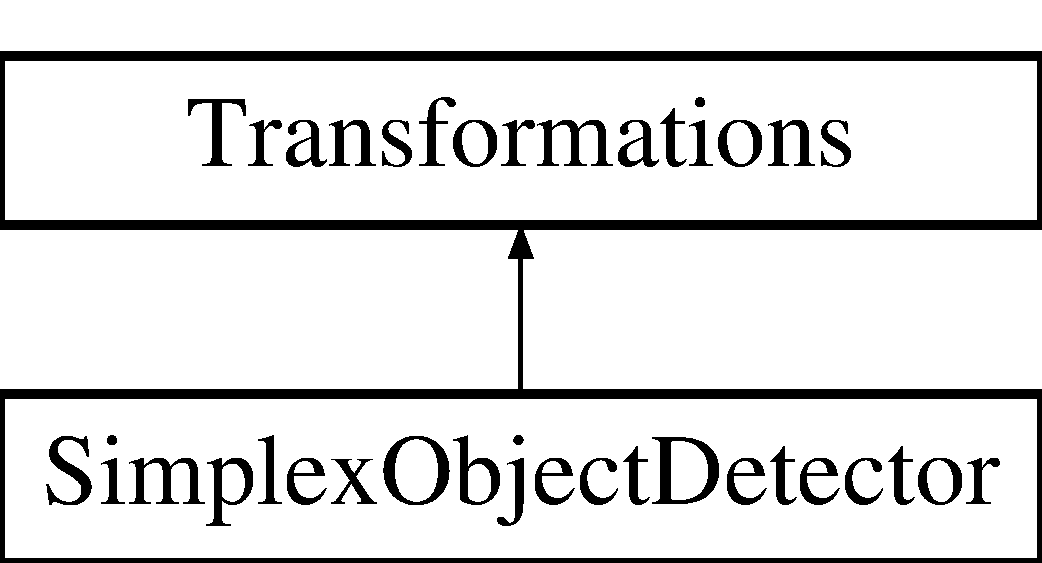
\includegraphics[height=2.000000cm]{class_simplex_object_detector}
\end{center}
\end{figure}
\subsection*{Public Member Functions}
\begin{DoxyCompactItemize}
\item 
\hyperlink{class_simplex_object_detector_a808e69553c4b8ff683e187416fde7f56}{Simplex\+Object\+Detector} (\hyperlink{class_distance_base}{Distance\+Base} $\ast$distance\+Measure)
\begin{DoxyCompactList}\small\item\em Constructor. \end{DoxyCompactList}\item 
\hyperlink{struct_a_i_s___options_1_1_location}{Location} \hyperlink{class_simplex_object_detector_a6b09b0c1629feffb2523d9ed6038545b}{find\+Object\+All\+Transformations} (\hyperlink{struct_a_i_s___options_1_1_location}{Location} predicted\+Location, Mat frame, vector$<$ Mat $>$ appearances, int $\ast$most\+Matched\+Appearance\+Index)
\begin{DoxyCompactList}\small\item\em Find the object using rotation and scale. \end{DoxyCompactList}\item 
\hyperlink{struct_a_i_s___options_1_1_location}{Location} \hyperlink{class_simplex_object_detector_ac6e9fcfe1427b93308b69f950d6ba88e}{find\+Object\+With\+Scale} (\hyperlink{struct_a_i_s___options_1_1_location}{Location} predicted\+Location, Mat frame, vector$<$ Mat $>$ appearances, int $\ast$most\+Matched\+Appearance\+Index)
\begin{DoxyCompactList}\small\item\em Finds the object using just the scale transformation. \end{DoxyCompactList}\item 
\hyperlink{struct_a_i_s___options_1_1_location}{Location} \hyperlink{class_simplex_object_detector_af245a74403f3b2098042b0e1e567e999}{find\+Object\+With\+Rotation} (\hyperlink{struct_a_i_s___options_1_1_location}{Location} predicted\+Location, Mat frame, vector$<$ Mat $>$ appearances, int $\ast$most\+Matched\+Appearance\+Index)
\begin{DoxyCompactList}\small\item\em Finds the object using just the rotation transformation. \end{DoxyCompactList}\item 
\hyperlink{struct_a_i_s___options_1_1_location}{Location} \hyperlink{class_simplex_object_detector_ae62a15fe369dfd1698358f2cb36e0d63}{find\+Object\+No\+Transformations} (\hyperlink{struct_a_i_s___options_1_1_location}{Location} predicted\+Location, Mat frame, vector$<$ Mat $>$ appearances, int $\ast$most\+Matched\+Appearance\+Index)
\begin{DoxyCompactList}\small\item\em Finds the object without the use of scale or rotation. \end{DoxyCompactList}\end{DoxyCompactItemize}
\subsection*{Additional Inherited Members}


\subsection{Detailed Description}
Uses the Simplex functionality of G\+S\+L to locate the object being tracked. 

\subsection{Constructor \& Destructor Documentation}
\hypertarget{class_simplex_object_detector_a808e69553c4b8ff683e187416fde7f56}{}\index{Simplex\+Object\+Detector@{Simplex\+Object\+Detector}!Simplex\+Object\+Detector@{Simplex\+Object\+Detector}}
\index{Simplex\+Object\+Detector@{Simplex\+Object\+Detector}!Simplex\+Object\+Detector@{Simplex\+Object\+Detector}}
\subsubsection[{Simplex\+Object\+Detector}]{\setlength{\rightskip}{0pt plus 5cm}Simplex\+Object\+Detector\+::\+Simplex\+Object\+Detector (
\begin{DoxyParamCaption}
\item[{{\bf Distance\+Base} $\ast$}]{distance\+Measure}
\end{DoxyParamCaption}
)}\label{class_simplex_object_detector_a808e69553c4b8ff683e187416fde7f56}


Constructor. 


\begin{DoxyParams}{Parameters}
{\em distance\+Measure} & \mbox{[}in\mbox{]} \\
\hline
\end{DoxyParams}


\subsection{Member Function Documentation}
\hypertarget{class_simplex_object_detector_a6b09b0c1629feffb2523d9ed6038545b}{}\index{Simplex\+Object\+Detector@{Simplex\+Object\+Detector}!find\+Object\+All\+Transformations@{find\+Object\+All\+Transformations}}
\index{find\+Object\+All\+Transformations@{find\+Object\+All\+Transformations}!Simplex\+Object\+Detector@{Simplex\+Object\+Detector}}
\subsubsection[{find\+Object\+All\+Transformations}]{\setlength{\rightskip}{0pt plus 5cm}Simplex\+Object\+Detector\+::find\+Object\+All\+Transformations (
\begin{DoxyParamCaption}
\item[{{\bf Location}}]{predicted\+Location, }
\item[{Mat}]{frame, }
\item[{vector$<$ Mat $>$}]{appearances, }
\item[{int $\ast$}]{most\+Matched\+Appearance\+Index}
\end{DoxyParamCaption}
)}\label{class_simplex_object_detector_a6b09b0c1629feffb2523d9ed6038545b}


Find the object using rotation and scale. 


\begin{DoxyParams}{Parameters}
{\em predicted\+Location} & \mbox{[}in\mbox{]} \+: The location to start looking for the object \\
\hline
{\em frame} & \mbox{[}in\mbox{]} \+: The image the search is being performed on \\
\hline
{\em appearances} & \mbox{[}in\mbox{]} \+: The apperances used to find the object in the frame \\
\hline
{\em most\+Matched\+Appearance\+Index} & \mbox{[}out\mbox{]} \\
\hline
\end{DoxyParams}
\begin{DoxyReturn}{Returns}
The location of the object. 
\end{DoxyReturn}
\hypertarget{class_simplex_object_detector_ae62a15fe369dfd1698358f2cb36e0d63}{}\index{Simplex\+Object\+Detector@{Simplex\+Object\+Detector}!find\+Object\+No\+Transformations@{find\+Object\+No\+Transformations}}
\index{find\+Object\+No\+Transformations@{find\+Object\+No\+Transformations}!Simplex\+Object\+Detector@{Simplex\+Object\+Detector}}
\subsubsection[{find\+Object\+No\+Transformations}]{\setlength{\rightskip}{0pt plus 5cm}Simplex\+Object\+Detector\+::find\+Object\+No\+Transformations (
\begin{DoxyParamCaption}
\item[{{\bf Location}}]{predicted\+Location, }
\item[{Mat}]{frame, }
\item[{vector$<$ Mat $>$}]{appearances, }
\item[{int $\ast$}]{most\+Matched\+Appearance\+Index}
\end{DoxyParamCaption}
)}\label{class_simplex_object_detector_ae62a15fe369dfd1698358f2cb36e0d63}


Finds the object without the use of scale or rotation. 


\begin{DoxyParams}{Parameters}
{\em predicted\+Location} & \mbox{[}in\mbox{]} \\
\hline
{\em frame} & \mbox{[}in\mbox{]} \\
\hline
{\em appearances} & \mbox{[}in\mbox{]} \\
\hline
{\em most\+Matched\+Appearance\+Index} & \mbox{[}out\mbox{]} \\
\hline
\end{DoxyParams}
\begin{DoxyReturn}{Returns}
The location of the object. 
\end{DoxyReturn}
\hypertarget{class_simplex_object_detector_af245a74403f3b2098042b0e1e567e999}{}\index{Simplex\+Object\+Detector@{Simplex\+Object\+Detector}!find\+Object\+With\+Rotation@{find\+Object\+With\+Rotation}}
\index{find\+Object\+With\+Rotation@{find\+Object\+With\+Rotation}!Simplex\+Object\+Detector@{Simplex\+Object\+Detector}}
\subsubsection[{find\+Object\+With\+Rotation}]{\setlength{\rightskip}{0pt plus 5cm}Simplex\+Object\+Detector\+::find\+Object\+With\+Rotation (
\begin{DoxyParamCaption}
\item[{{\bf Location}}]{predicted\+Location, }
\item[{Mat}]{frame, }
\item[{vector$<$ Mat $>$}]{appearances, }
\item[{int $\ast$}]{most\+Matched\+Appearance\+Index}
\end{DoxyParamCaption}
)}\label{class_simplex_object_detector_af245a74403f3b2098042b0e1e567e999}


Finds the object using just the rotation transformation. 


\begin{DoxyParams}{Parameters}
{\em predicted\+Location} & \mbox{[}in\mbox{]} \\
\hline
{\em frame} & \mbox{[}in\mbox{]} \\
\hline
{\em appearances} & \mbox{[}in\mbox{]} \\
\hline
{\em most\+Matched\+Appearance\+Index} & \mbox{[}out\mbox{]} \\
\hline
\end{DoxyParams}
\begin{DoxyReturn}{Returns}
The location of the object. 
\end{DoxyReturn}
\hypertarget{class_simplex_object_detector_ac6e9fcfe1427b93308b69f950d6ba88e}{}\index{Simplex\+Object\+Detector@{Simplex\+Object\+Detector}!find\+Object\+With\+Scale@{find\+Object\+With\+Scale}}
\index{find\+Object\+With\+Scale@{find\+Object\+With\+Scale}!Simplex\+Object\+Detector@{Simplex\+Object\+Detector}}
\subsubsection[{find\+Object\+With\+Scale}]{\setlength{\rightskip}{0pt plus 5cm}Simplex\+Object\+Detector\+::find\+Object\+With\+Scale (
\begin{DoxyParamCaption}
\item[{{\bf Location}}]{predicted\+Location, }
\item[{Mat}]{frame, }
\item[{vector$<$ Mat $>$}]{appearances, }
\item[{int $\ast$}]{most\+Matched\+Appearance\+Index}
\end{DoxyParamCaption}
)}\label{class_simplex_object_detector_ac6e9fcfe1427b93308b69f950d6ba88e}


Finds the object using just the scale transformation. 


\begin{DoxyParams}{Parameters}
{\em predicted\+Location} & \mbox{[}in\mbox{]} \\
\hline
{\em frame} & \mbox{[}in\mbox{]} \\
\hline
{\em appearances} & \mbox{[}in\mbox{]} \\
\hline
{\em most\+Matched\+Appearance\+Index} & \mbox{[}out\mbox{]} \\
\hline
\end{DoxyParams}
\begin{DoxyReturn}{Returns}
The location of the object. 
\end{DoxyReturn}


The documentation for this class was generated from the following files\+:\begin{DoxyCompactItemize}
\item 
simplex\+Object\+Detector.\+h\item 
simplex\+Object\+Detector.\+cpp\end{DoxyCompactItemize}

\hypertarget{class_sum_of_squared_difference}{}\section{Sum\+Of\+Squared\+Difference Class Reference}
\label{class_sum_of_squared_difference}\index{Sum\+Of\+Squared\+Difference@{Sum\+Of\+Squared\+Difference}}


Used to calculate the Sum Of Squared Difference between two appearances.  




{\ttfamily \#include $<$sum\+Of\+Squared\+Difference.\+h$>$}

Inheritance diagram for Sum\+Of\+Squared\+Difference\+:\begin{figure}[H]
\begin{center}
\leavevmode
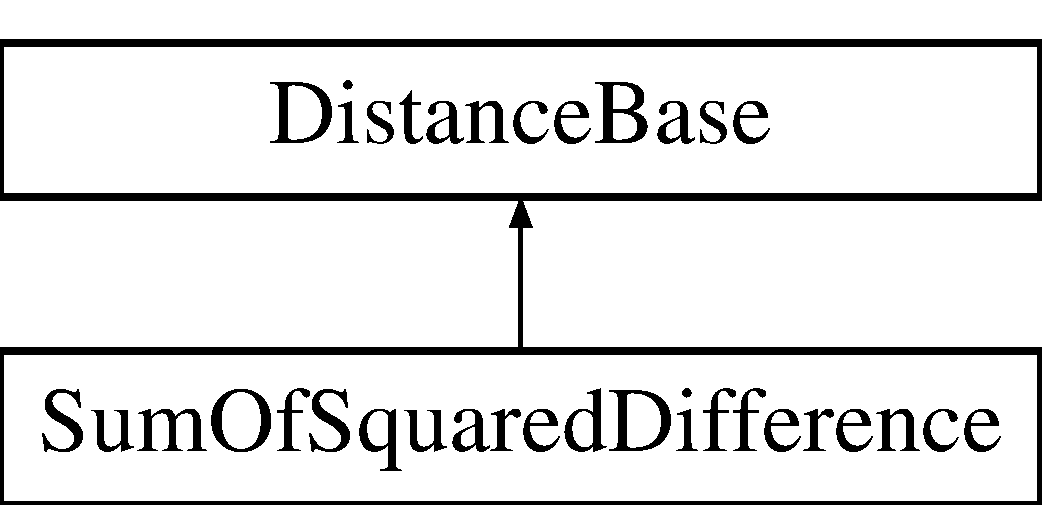
\includegraphics[height=2.000000cm]{class_sum_of_squared_difference}
\end{center}
\end{figure}
\subsection*{Public Member Functions}
\begin{DoxyCompactItemize}
\item 
\hyperlink{class_sum_of_squared_difference_af922c956c34c21fd1f361ff17c8e74dd}{Sum\+Of\+Squared\+Difference} (Mat frame, Mat appearance)
\begin{DoxyCompactList}\small\item\em Will set the max\+Distance the unnormalised S\+S\+D should return. \end{DoxyCompactList}\item 
\hypertarget{class_sum_of_squared_difference_ac9d3e8ddd24e68dab66f712f7810e6bd}{}\hyperlink{class_sum_of_squared_difference_ac9d3e8ddd24e68dab66f712f7810e6bd}{Sum\+Of\+Squared\+Difference} ()\label{class_sum_of_squared_difference_ac9d3e8ddd24e68dab66f712f7810e6bd}

\begin{DoxyCompactList}\small\item\em Used by the unit tests. \end{DoxyCompactList}\item 
double \hyperlink{class_sum_of_squared_difference_acd647d0817edf9cce383caa657ab46fa}{get\+Distance} (Mat image, Mat appearance)
\begin{DoxyCompactList}\small\item\em Calculates the distance between the image and the appearance. \end{DoxyCompactList}\end{DoxyCompactItemize}
\subsection*{Additional Inherited Members}


\subsection{Detailed Description}
Used to calculate the Sum Of Squared Difference between two appearances. 

\subsection{Constructor \& Destructor Documentation}
\hypertarget{class_sum_of_squared_difference_af922c956c34c21fd1f361ff17c8e74dd}{}\index{Sum\+Of\+Squared\+Difference@{Sum\+Of\+Squared\+Difference}!Sum\+Of\+Squared\+Difference@{Sum\+Of\+Squared\+Difference}}
\index{Sum\+Of\+Squared\+Difference@{Sum\+Of\+Squared\+Difference}!Sum\+Of\+Squared\+Difference@{Sum\+Of\+Squared\+Difference}}
\subsubsection[{Sum\+Of\+Squared\+Difference}]{\setlength{\rightskip}{0pt plus 5cm}Sum\+Of\+Squared\+Difference\+::\+Sum\+Of\+Squared\+Difference (
\begin{DoxyParamCaption}
\item[{Mat}]{frame, }
\item[{Mat}]{appearance}
\end{DoxyParamCaption}
)}\label{class_sum_of_squared_difference_af922c956c34c21fd1f361ff17c8e74dd}


Will set the max\+Distance the unnormalised S\+S\+D should return. 


\begin{DoxyParams}{Parameters}
{\em frame} & \mbox{[}in\mbox{]}\+: The frame whch the appearance has been selected from \\
\hline
{\em appearance} & \mbox{[}in\mbox{]}\+: The appearance the user has selected \\
\hline
\end{DoxyParams}


\subsection{Member Function Documentation}
\hypertarget{class_sum_of_squared_difference_acd647d0817edf9cce383caa657ab46fa}{}\index{Sum\+Of\+Squared\+Difference@{Sum\+Of\+Squared\+Difference}!get\+Distance@{get\+Distance}}
\index{get\+Distance@{get\+Distance}!Sum\+Of\+Squared\+Difference@{Sum\+Of\+Squared\+Difference}}
\subsubsection[{get\+Distance}]{\setlength{\rightskip}{0pt plus 5cm}Sum\+Of\+Squared\+Difference\+::get\+Distance (
\begin{DoxyParamCaption}
\item[{Mat}]{image, }
\item[{Mat}]{appearance}
\end{DoxyParamCaption}
)\hspace{0.3cm}{\ttfamily [virtual]}}\label{class_sum_of_squared_difference_acd647d0817edf9cce383caa657ab46fa}


Calculates the distance between the image and the appearance. 


\begin{DoxyParams}{Parameters}
{\em image} & \mbox{[}in\mbox{]} \\
\hline
{\em appearance} & \mbox{[}in\mbox{]} \\
\hline
\end{DoxyParams}
\begin{DoxyReturn}{Returns}
The normalised Euclidean distance (value between 0 and 1). 
\end{DoxyReturn}


Implements \hyperlink{class_distance_base_aafc76227a800dd0827bedefded215646}{Distance\+Base}.



The documentation for this class was generated from the following files\+:\begin{DoxyCompactItemize}
\item 
Distance\+Measures/\hyperlink{sum_of_squared_difference_8h}{sum\+Of\+Squared\+Difference.\+h}\item 
Distance\+Measures/\hyperlink{sum_of_squared_difference_8cpp}{sum\+Of\+Squared\+Difference.\+cpp}\end{DoxyCompactItemize}

\hypertarget{class_tracking_and_detection}{}\section{Tracking\+And\+Detection Class Reference}
\label{class_tracking_and_detection}\index{Tracking\+And\+Detection@{Tracking\+And\+Detection}}


The class that handles and runs the tracking and detection of an object.  




{\ttfamily \#include $<$tracking\+And\+Detection.\+h$>$}

Inheritance diagram for Tracking\+And\+Detection\+:\begin{figure}[H]
\begin{center}
\leavevmode
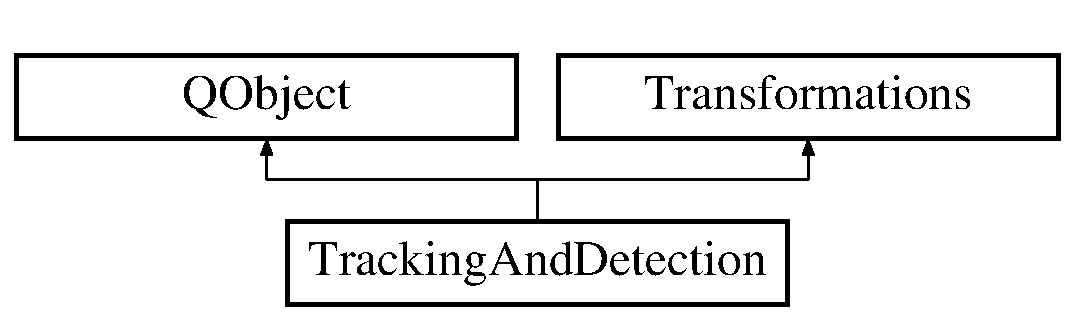
\includegraphics[height=2.000000cm]{class_tracking_and_detection}
\end{center}
\end{figure}
\subsection*{Public Slots}
\begin{DoxyCompactItemize}
\item 
\hypertarget{class_tracking_and_detection_a8ca5a5cadb863fb27398d30726f41deb}{}void {\bfseries distance\+Measure\+Changed} (Distance\+Measure\+Type distance\+Measure\+Type)\label{class_tracking_and_detection_a8ca5a5cadb863fb27398d30726f41deb}

\item 
void \hyperlink{class_tracking_and_detection_a8ebab1c0f4615155db5fc87f477b5133}{use\+Rotation\+Changed} (bool use\+Rotation)
\item 
void \hyperlink{class_tracking_and_detection_a0288d1f356c9eaa5bf6074b6eef5b8d8}{use\+Scale\+Changed} (bool use\+Scale)
\item 
void \hyperlink{class_tracking_and_detection_a8c9a4536964366076a76ba0bb52c5c5f}{which\+A\+R\+Bs\+To\+Search\+With\+Changed} (A\+R\+Bs\+To\+Search\+With which\+A\+R\+Bs\+To\+Search\+With)
\item 
void \hyperlink{class_tracking_and_detection_a56ae5d619bb8f38f58c9c2d58a1c9590}{use\+Predicted\+Location\+Changed} (bool use\+Predicted\+Location)
\item 
void \hyperlink{class_tracking_and_detection_ac115a3770df344a0b5dfbd626094a85d}{state\+Changed} (Program\+State state)
\item 
\hypertarget{class_tracking_and_detection_a0fb0b246ec71cb4efdf55114d54f733d}{}void {\bfseries get\+Network} ()\label{class_tracking_and_detection_a0fb0b246ec71cb4efdf55114d54f733d}

\item 
void \hyperlink{class_tracking_and_detection_aad697a8cd333e516098e44c5bab33bab}{change\+Video\+Config\+File\+Path} (string file\+Path\+Name)
\begin{DoxyCompactList}\small\item\em Called when the user selects the video config file that should be used. \end{DoxyCompactList}\item 
void \hyperlink{class_tracking_and_detection_a88b3a6b164c4e3038090d2e8b9069914}{reset} (Video\+Input\+Type input\+Type)
\begin{DoxyCompactList}\small\item\em When a new video type is selected by the user we need to reset the tracking. \end{DoxyCompactList}\item 
\hypertarget{class_tracking_and_detection_a3d909c374ab512204cc78e85168f9ecc}{}void {\bfseries run\+Video\+Feed} ()\label{class_tracking_and_detection_a3d909c374ab512204cc78e85168f9ecc}

\item 
void \hyperlink{class_tracking_and_detection_a8bb8cf4b4bf79c3605c450f0a998ff63}{initialise\+Tracking\+From\+Position} (int x, int y, int width, int height)
\begin{DoxyCompactList}\small\item\em Initialises the artifical immunue network with the initial appearance. \end{DoxyCompactList}\item 
void \hyperlink{class_tracking_and_detection_a8eafd41240df57ed65ae67550f18d540}{stimulation\+Threshold\+Changed} (double stimulation\+Threshold)
\item 
void \hyperlink{class_tracking_and_detection_aa2c2aa4f8901f92b101a99013eb55551}{object\+Threshold\+Changed} (double object\+Threshold)
\end{DoxyCompactItemize}
\subsection*{Signals}
\begin{DoxyCompactItemize}
\item 
void \hyperlink{class_tracking_and_detection_a218aab354939b487503031ddc2b913d3}{update\+Image} (uchar $\ast$data, int cols, int rows)
\begin{DoxyCompactList}\small\item\em Allows the qt\+Widget\+Image\+Display to show the image. \end{DoxyCompactList}\item 
void \hyperlink{class_tracking_and_detection_af709dac7ba7d396a837ae9fe3997dd7a}{update\+Objects\+Position} (int x, int y, int rotation, int width, int height)
\begin{DoxyCompactList}\small\item\em Allows the U\+I to show the objects location. \end{DoxyCompactList}\item 
void \hyperlink{class_tracking_and_detection_a3526dce8ac46f591dde4725d33ba8869}{update\+Num\+A\+R\+Bs} (int num\+A\+R\+Bs)
\item 
\hypertarget{class_tracking_and_detection_a1bce1d598c2d2a53d3f41c0a25b91037}{}void {\bfseries grab\+Video\+File\+Config} ()\label{class_tracking_and_detection_a1bce1d598c2d2a53d3f41c0a25b91037}

\item 
void \hyperlink{class_tracking_and_detection_a96867b74b33b67c0a8ddb4ebd07af60e}{set\+Network} (\hyperlink{class_network}{Network} $\ast$network)
\begin{DoxyCompactList}\small\item\em Allows the network to be saved to file. \end{DoxyCompactList}\end{DoxyCompactItemize}
\subsection*{Public Member Functions}
\begin{DoxyCompactItemize}
\item 
\hyperlink{class_tracking_and_detection_ae9c1d968d4fd3b298fb3ba423de5a4f0}{Tracking\+And\+Detection} ()
\begin{DoxyCompactList}\small\item\em Default constructor. \end{DoxyCompactList}\end{DoxyCompactItemize}
\subsection*{Additional Inherited Members}


\subsection{Detailed Description}
The class that handles and runs the tracking and detection of an object. 

\subsection{Constructor \& Destructor Documentation}
\hypertarget{class_tracking_and_detection_ae9c1d968d4fd3b298fb3ba423de5a4f0}{}\index{Tracking\+And\+Detection@{Tracking\+And\+Detection}!Tracking\+And\+Detection@{Tracking\+And\+Detection}}
\index{Tracking\+And\+Detection@{Tracking\+And\+Detection}!Tracking\+And\+Detection@{Tracking\+And\+Detection}}
\subsubsection[{Tracking\+And\+Detection}]{\setlength{\rightskip}{0pt plus 5cm}Tracking\+And\+Detection\+::\+Tracking\+And\+Detection (
\begin{DoxyParamCaption}
{}
\end{DoxyParamCaption}
)}\label{class_tracking_and_detection_ae9c1d968d4fd3b298fb3ba423de5a4f0}


Default constructor. 


\begin{DoxyParams}{Parameters}
{\em input\+Type} & \\
\hline
\end{DoxyParams}


\subsection{Member Function Documentation}
\hypertarget{class_tracking_and_detection_aad697a8cd333e516098e44c5bab33bab}{}\index{Tracking\+And\+Detection@{Tracking\+And\+Detection}!change\+Video\+Config\+File\+Path@{change\+Video\+Config\+File\+Path}}
\index{change\+Video\+Config\+File\+Path@{change\+Video\+Config\+File\+Path}!Tracking\+And\+Detection@{Tracking\+And\+Detection}}
\subsubsection[{change\+Video\+Config\+File\+Path}]{\setlength{\rightskip}{0pt plus 5cm}Tracking\+And\+Detection\+::change\+Video\+Config\+File\+Path (
\begin{DoxyParamCaption}
\item[{string}]{file\+Path\+Name}
\end{DoxyParamCaption}
)\hspace{0.3cm}{\ttfamily [slot]}}\label{class_tracking_and_detection_aad697a8cd333e516098e44c5bab33bab}


Called when the user selects the video config file that should be used. 


\begin{DoxyParams}{Parameters}
{\em file\+Path\+Name} & \mbox{[}in\mbox{]} \\
\hline
\end{DoxyParams}
\hypertarget{class_tracking_and_detection_a8bb8cf4b4bf79c3605c450f0a998ff63}{}\index{Tracking\+And\+Detection@{Tracking\+And\+Detection}!initialise\+Tracking\+From\+Position@{initialise\+Tracking\+From\+Position}}
\index{initialise\+Tracking\+From\+Position@{initialise\+Tracking\+From\+Position}!Tracking\+And\+Detection@{Tracking\+And\+Detection}}
\subsubsection[{initialise\+Tracking\+From\+Position}]{\setlength{\rightskip}{0pt plus 5cm}Tracking\+And\+Detection\+::initialise\+Tracking\+From\+Position (
\begin{DoxyParamCaption}
\item[{int}]{x, }
\item[{int}]{y, }
\item[{int}]{width, }
\item[{int}]{height}
\end{DoxyParamCaption}
)\hspace{0.3cm}{\ttfamily [slot]}}\label{class_tracking_and_detection_a8bb8cf4b4bf79c3605c450f0a998ff63}


Initialises the artifical immunue network with the initial appearance. 


\begin{DoxyParams}{Parameters}
{\em x} & \mbox{[}in\mbox{]} \\
\hline
{\em y} & \mbox{[}in\mbox{]} \\
\hline
{\em width} & \mbox{[}in\mbox{]} \\
\hline
{\em height} & \mbox{[}in\mbox{]} \\
\hline
\end{DoxyParams}
\hypertarget{class_tracking_and_detection_aa2c2aa4f8901f92b101a99013eb55551}{}\index{Tracking\+And\+Detection@{Tracking\+And\+Detection}!object\+Threshold\+Changed@{object\+Threshold\+Changed}}
\index{object\+Threshold\+Changed@{object\+Threshold\+Changed}!Tracking\+And\+Detection@{Tracking\+And\+Detection}}
\subsubsection[{object\+Threshold\+Changed}]{\setlength{\rightskip}{0pt plus 5cm}Tracking\+And\+Detection\+::object\+Threshold\+Changed (
\begin{DoxyParamCaption}
\item[{double}]{object\+Threshold}
\end{DoxyParamCaption}
)\hspace{0.3cm}{\ttfamily [slot]}}\label{class_tracking_and_detection_aa2c2aa4f8901f92b101a99013eb55551}

\begin{DoxyParams}{Parameters}
{\em object\+Threshold} & \mbox{[}in\mbox{]} \\
\hline
\end{DoxyParams}
\hypertarget{class_tracking_and_detection_a88b3a6b164c4e3038090d2e8b9069914}{}\index{Tracking\+And\+Detection@{Tracking\+And\+Detection}!reset@{reset}}
\index{reset@{reset}!Tracking\+And\+Detection@{Tracking\+And\+Detection}}
\subsubsection[{reset}]{\setlength{\rightskip}{0pt plus 5cm}Tracking\+And\+Detection\+::reset (
\begin{DoxyParamCaption}
\item[{Video\+Input\+Type}]{input\+Type}
\end{DoxyParamCaption}
)\hspace{0.3cm}{\ttfamily [slot]}}\label{class_tracking_and_detection_a88b3a6b164c4e3038090d2e8b9069914}


When a new video type is selected by the user we need to reset the tracking. 


\begin{DoxyParams}{Parameters}
{\em input\+Type} & \mbox{[}in\mbox{]} \+: What video source should be used \\
\hline
\end{DoxyParams}
\hypertarget{class_tracking_and_detection_a96867b74b33b67c0a8ddb4ebd07af60e}{}\index{Tracking\+And\+Detection@{Tracking\+And\+Detection}!set\+Network@{set\+Network}}
\index{set\+Network@{set\+Network}!Tracking\+And\+Detection@{Tracking\+And\+Detection}}
\subsubsection[{set\+Network}]{\setlength{\rightskip}{0pt plus 5cm}Tracking\+And\+Detection\+::set\+Network (
\begin{DoxyParamCaption}
\item[{{\bf Network} $\ast$}]{network}
\end{DoxyParamCaption}
)\hspace{0.3cm}{\ttfamily [signal]}}\label{class_tracking_and_detection_a96867b74b33b67c0a8ddb4ebd07af60e}


Allows the network to be saved to file. 


\begin{DoxyParams}{Parameters}
{\em network} & \mbox{[}in\mbox{]} \\
\hline
\end{DoxyParams}
\hypertarget{class_tracking_and_detection_ac115a3770df344a0b5dfbd626094a85d}{}\index{Tracking\+And\+Detection@{Tracking\+And\+Detection}!state\+Changed@{state\+Changed}}
\index{state\+Changed@{state\+Changed}!Tracking\+And\+Detection@{Tracking\+And\+Detection}}
\subsubsection[{state\+Changed}]{\setlength{\rightskip}{0pt plus 5cm}Tracking\+And\+Detection\+::state\+Changed (
\begin{DoxyParamCaption}
\item[{Program\+State}]{state}
\end{DoxyParamCaption}
)\hspace{0.3cm}{\ttfamily [slot]}}\label{class_tracking_and_detection_ac115a3770df344a0b5dfbd626094a85d}

\begin{DoxyParams}{Parameters}
{\em state} & \mbox{[}in\mbox{]} \\
\hline
\end{DoxyParams}
\hypertarget{class_tracking_and_detection_a8eafd41240df57ed65ae67550f18d540}{}\index{Tracking\+And\+Detection@{Tracking\+And\+Detection}!stimulation\+Threshold\+Changed@{stimulation\+Threshold\+Changed}}
\index{stimulation\+Threshold\+Changed@{stimulation\+Threshold\+Changed}!Tracking\+And\+Detection@{Tracking\+And\+Detection}}
\subsubsection[{stimulation\+Threshold\+Changed}]{\setlength{\rightskip}{0pt plus 5cm}Tracking\+And\+Detection\+::stimulation\+Threshold\+Changed (
\begin{DoxyParamCaption}
\item[{double}]{stimulation\+Threshold}
\end{DoxyParamCaption}
)\hspace{0.3cm}{\ttfamily [slot]}}\label{class_tracking_and_detection_a8eafd41240df57ed65ae67550f18d540}

\begin{DoxyParams}{Parameters}
{\em stimulation\+Threshold} & \mbox{[}in\mbox{]} \\
\hline
\end{DoxyParams}
\hypertarget{class_tracking_and_detection_a218aab354939b487503031ddc2b913d3}{}\index{Tracking\+And\+Detection@{Tracking\+And\+Detection}!update\+Image@{update\+Image}}
\index{update\+Image@{update\+Image}!Tracking\+And\+Detection@{Tracking\+And\+Detection}}
\subsubsection[{update\+Image}]{\setlength{\rightskip}{0pt plus 5cm}Tracking\+And\+Detection\+::update\+Image (
\begin{DoxyParamCaption}
\item[{uchar $\ast$}]{data, }
\item[{int}]{cols, }
\item[{int}]{rows}
\end{DoxyParamCaption}
)\hspace{0.3cm}{\ttfamily [signal]}}\label{class_tracking_and_detection_a218aab354939b487503031ddc2b913d3}


Allows the qt\+Widget\+Image\+Display to show the image. 


\begin{DoxyParams}{Parameters}
{\em data} & \mbox{[}in\mbox{]} \\
\hline
{\em cols} & \mbox{[}in\mbox{]} \\
\hline
{\em rows} & \mbox{[}in\mbox{]} \\
\hline
\end{DoxyParams}
\hypertarget{class_tracking_and_detection_a3526dce8ac46f591dde4725d33ba8869}{}\index{Tracking\+And\+Detection@{Tracking\+And\+Detection}!update\+Num\+A\+R\+Bs@{update\+Num\+A\+R\+Bs}}
\index{update\+Num\+A\+R\+Bs@{update\+Num\+A\+R\+Bs}!Tracking\+And\+Detection@{Tracking\+And\+Detection}}
\subsubsection[{update\+Num\+A\+R\+Bs}]{\setlength{\rightskip}{0pt plus 5cm}Tracking\+And\+Detection\+::update\+Num\+A\+R\+Bs (
\begin{DoxyParamCaption}
\item[{int}]{num\+A\+R\+Bs}
\end{DoxyParamCaption}
)\hspace{0.3cm}{\ttfamily [signal]}}\label{class_tracking_and_detection_a3526dce8ac46f591dde4725d33ba8869}

\begin{DoxyParams}{Parameters}
{\em num\+A\+R\+Bs} & \mbox{[}in\mbox{]} \\
\hline
\end{DoxyParams}
\hypertarget{class_tracking_and_detection_af709dac7ba7d396a837ae9fe3997dd7a}{}\index{Tracking\+And\+Detection@{Tracking\+And\+Detection}!update\+Objects\+Position@{update\+Objects\+Position}}
\index{update\+Objects\+Position@{update\+Objects\+Position}!Tracking\+And\+Detection@{Tracking\+And\+Detection}}
\subsubsection[{update\+Objects\+Position}]{\setlength{\rightskip}{0pt plus 5cm}Tracking\+And\+Detection\+::update\+Objects\+Position (
\begin{DoxyParamCaption}
\item[{int}]{x, }
\item[{int}]{y, }
\item[{int}]{rotation, }
\item[{int}]{width, }
\item[{int}]{height}
\end{DoxyParamCaption}
)\hspace{0.3cm}{\ttfamily [signal]}}\label{class_tracking_and_detection_af709dac7ba7d396a837ae9fe3997dd7a}


Allows the U\+I to show the objects location. 


\begin{DoxyParams}{Parameters}
{\em x} & \mbox{[}in\mbox{]} \\
\hline
{\em y} & \mbox{[}in\mbox{]} \\
\hline
{\em rotation} & \mbox{[}in\mbox{]} \\
\hline
{\em width} & \mbox{[}in\mbox{]} \\
\hline
{\em height} & \mbox{[}in\mbox{]} \\
\hline
\end{DoxyParams}
\hypertarget{class_tracking_and_detection_a56ae5d619bb8f38f58c9c2d58a1c9590}{}\index{Tracking\+And\+Detection@{Tracking\+And\+Detection}!use\+Predicted\+Location\+Changed@{use\+Predicted\+Location\+Changed}}
\index{use\+Predicted\+Location\+Changed@{use\+Predicted\+Location\+Changed}!Tracking\+And\+Detection@{Tracking\+And\+Detection}}
\subsubsection[{use\+Predicted\+Location\+Changed}]{\setlength{\rightskip}{0pt plus 5cm}Tracking\+And\+Detection\+::use\+Predicted\+Location\+Changed (
\begin{DoxyParamCaption}
\item[{bool}]{use\+Predicted\+Location}
\end{DoxyParamCaption}
)\hspace{0.3cm}{\ttfamily [slot]}}\label{class_tracking_and_detection_a56ae5d619bb8f38f58c9c2d58a1c9590}

\begin{DoxyParams}{Parameters}
{\em use\+Predicted\+Location} & \mbox{[}in\mbox{]} \\
\hline
\end{DoxyParams}
\hypertarget{class_tracking_and_detection_a8ebab1c0f4615155db5fc87f477b5133}{}\index{Tracking\+And\+Detection@{Tracking\+And\+Detection}!use\+Rotation\+Changed@{use\+Rotation\+Changed}}
\index{use\+Rotation\+Changed@{use\+Rotation\+Changed}!Tracking\+And\+Detection@{Tracking\+And\+Detection}}
\subsubsection[{use\+Rotation\+Changed}]{\setlength{\rightskip}{0pt plus 5cm}Tracking\+And\+Detection\+::use\+Rotation\+Changed (
\begin{DoxyParamCaption}
\item[{bool}]{use\+Rotation}
\end{DoxyParamCaption}
)\hspace{0.3cm}{\ttfamily [slot]}}\label{class_tracking_and_detection_a8ebab1c0f4615155db5fc87f477b5133}

\begin{DoxyParams}{Parameters}
{\em use\+Rotation} & \mbox{[}in\mbox{]} \\
\hline
\end{DoxyParams}
\hypertarget{class_tracking_and_detection_a0288d1f356c9eaa5bf6074b6eef5b8d8}{}\index{Tracking\+And\+Detection@{Tracking\+And\+Detection}!use\+Scale\+Changed@{use\+Scale\+Changed}}
\index{use\+Scale\+Changed@{use\+Scale\+Changed}!Tracking\+And\+Detection@{Tracking\+And\+Detection}}
\subsubsection[{use\+Scale\+Changed}]{\setlength{\rightskip}{0pt plus 5cm}Tracking\+And\+Detection\+::use\+Scale\+Changed (
\begin{DoxyParamCaption}
\item[{bool}]{use\+Scale}
\end{DoxyParamCaption}
)\hspace{0.3cm}{\ttfamily [slot]}}\label{class_tracking_and_detection_a0288d1f356c9eaa5bf6074b6eef5b8d8}

\begin{DoxyParams}{Parameters}
{\em use\+Scale} & \mbox{[}in\mbox{]} \\
\hline
\end{DoxyParams}
\hypertarget{class_tracking_and_detection_a8c9a4536964366076a76ba0bb52c5c5f}{}\index{Tracking\+And\+Detection@{Tracking\+And\+Detection}!which\+A\+R\+Bs\+To\+Search\+With\+Changed@{which\+A\+R\+Bs\+To\+Search\+With\+Changed}}
\index{which\+A\+R\+Bs\+To\+Search\+With\+Changed@{which\+A\+R\+Bs\+To\+Search\+With\+Changed}!Tracking\+And\+Detection@{Tracking\+And\+Detection}}
\subsubsection[{which\+A\+R\+Bs\+To\+Search\+With\+Changed}]{\setlength{\rightskip}{0pt plus 5cm}Tracking\+And\+Detection\+::which\+A\+R\+Bs\+To\+Search\+With\+Changed (
\begin{DoxyParamCaption}
\item[{A\+R\+Bs\+To\+Search\+With}]{which\+A\+R\+Bs\+To\+Search\+With}
\end{DoxyParamCaption}
)\hspace{0.3cm}{\ttfamily [slot]}}\label{class_tracking_and_detection_a8c9a4536964366076a76ba0bb52c5c5f}

\begin{DoxyParams}{Parameters}
{\em which\+A\+R\+Bs\+To\+Search\+With} & \mbox{[}in\mbox{]} \\
\hline
\end{DoxyParams}


The documentation for this class was generated from the following files\+:\begin{DoxyCompactItemize}
\item 
\hyperlink{tracking_and_detection_8h}{tracking\+And\+Detection.\+h}\item 
\hyperlink{tracking_and_detection_8cpp}{tracking\+And\+Detection.\+cpp}\end{DoxyCompactItemize}

\hypertarget{class_transformations}{}\section{Transformations Class Reference}
\label{class_transformations}\index{Transformations@{Transformations}}


Performs the rotation of a position and an image. Stopped code being repeated in several places.  




{\ttfamily \#include $<$transformations.\+h$>$}

Inheritance diagram for Transformations\+:\begin{figure}[H]
\begin{center}
\leavevmode
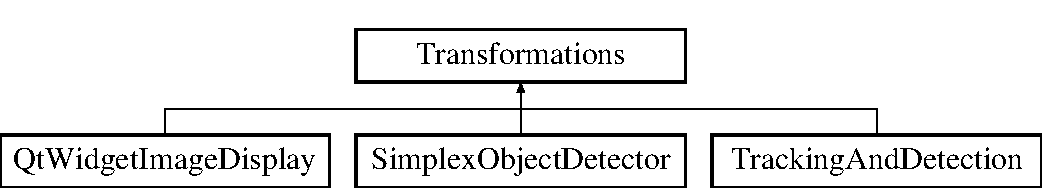
\includegraphics[height=2.000000cm]{class_transformations}
\end{center}
\end{figure}
\subsection*{Protected Member Functions}
\begin{DoxyCompactItemize}
\item 
void \hyperlink{class_transformations_ad7854509a197c02fe33df60cda622c11}{rotate\+Frame\+And\+Position} (int rotation, Mat $\ast$frame, int $\ast$x, int $\ast$y)
\item 
void \hyperlink{class_transformations_a9225a5452e0a3943fe7f91024538d5c3}{rotate\+Frame} (int rotation, Mat $\ast$frame)
\item 
void \hyperlink{class_transformations_a2f3d48d1535caddb0af4b619e9bce694}{rotate\+Position} (int degrees, int $\ast$x, int $\ast$y, int rotation\+Center\+X, int rotation\+Center\+Y)
\end{DoxyCompactItemize}


\subsection{Detailed Description}
Performs the rotation of a position and an image. Stopped code being repeated in several places. 

\subsection{Member Function Documentation}
\hypertarget{class_transformations_a9225a5452e0a3943fe7f91024538d5c3}{}\index{Transformations@{Transformations}!rotate\+Frame@{rotate\+Frame}}
\index{rotate\+Frame@{rotate\+Frame}!Transformations@{Transformations}}
\subsubsection[{rotate\+Frame}]{\setlength{\rightskip}{0pt plus 5cm}Transformations\+::rotate\+Frame (
\begin{DoxyParamCaption}
\item[{int}]{rotation, }
\item[{Mat $\ast$}]{frame}
\end{DoxyParamCaption}
)\hspace{0.3cm}{\ttfamily [protected]}}\label{class_transformations_a9225a5452e0a3943fe7f91024538d5c3}

\begin{DoxyParams}{Parameters}
{\em rotation} & \mbox{[}in\mbox{]} \\
\hline
{\em frame} & \mbox{[}in, out\mbox{]} \\
\hline
\end{DoxyParams}
\hypertarget{class_transformations_ad7854509a197c02fe33df60cda622c11}{}\index{Transformations@{Transformations}!rotate\+Frame\+And\+Position@{rotate\+Frame\+And\+Position}}
\index{rotate\+Frame\+And\+Position@{rotate\+Frame\+And\+Position}!Transformations@{Transformations}}
\subsubsection[{rotate\+Frame\+And\+Position}]{\setlength{\rightskip}{0pt plus 5cm}Transformations\+::rotate\+Frame\+And\+Position (
\begin{DoxyParamCaption}
\item[{int}]{rotation, }
\item[{Mat $\ast$}]{frame, }
\item[{int $\ast$}]{x, }
\item[{int $\ast$}]{y}
\end{DoxyParamCaption}
)\hspace{0.3cm}{\ttfamily [protected]}}\label{class_transformations_ad7854509a197c02fe33df60cda622c11}

\begin{DoxyParams}{Parameters}
{\em rotation} & \mbox{[}in\mbox{]} \\
\hline
{\em frame} & \mbox{[}in, out\mbox{]} \\
\hline
{\em x} & \mbox{[}in, out\mbox{]} \\
\hline
{\em y} & \mbox{[}in, out\mbox{]} \\
\hline
\end{DoxyParams}
\hypertarget{class_transformations_a2f3d48d1535caddb0af4b619e9bce694}{}\index{Transformations@{Transformations}!rotate\+Position@{rotate\+Position}}
\index{rotate\+Position@{rotate\+Position}!Transformations@{Transformations}}
\subsubsection[{rotate\+Position}]{\setlength{\rightskip}{0pt plus 5cm}Transformations\+::rotate\+Position (
\begin{DoxyParamCaption}
\item[{int}]{degrees, }
\item[{int $\ast$}]{x, }
\item[{int $\ast$}]{y, }
\item[{int}]{rotation\+Center\+X, }
\item[{int}]{rotation\+Center\+Y}
\end{DoxyParamCaption}
)\hspace{0.3cm}{\ttfamily [protected]}}\label{class_transformations_a2f3d48d1535caddb0af4b619e9bce694}

\begin{DoxyParams}{Parameters}
{\em degrees} & \mbox{[}in\mbox{]} \\
\hline
{\em x} & \mbox{[}in, out\mbox{]} \\
\hline
{\em y} & \mbox{[}in, out\mbox{]} \\
\hline
{\em rotation\+Center\+X} & \mbox{[}in\mbox{]} \\
\hline
{\em rotation\+Center\+Y} & \mbox{[}in\mbox{]} \\
\hline
\end{DoxyParams}


The documentation for this class was generated from the following files\+:\begin{DoxyCompactItemize}
\item 
\hyperlink{transformations_8h}{transformations.\+h}\item 
transformations.\+cpp\end{DoxyCompactItemize}

\hypertarget{class_video_file_input}{}\section{Video\+File\+Input Class Reference}
\label{class_video_file_input}\index{Video\+File\+Input@{Video\+File\+Input}}


Allows the video feed to come from a video file.  




{\ttfamily \#include $<$video\+File\+Input.\+h$>$}

Inheritance diagram for Video\+File\+Input\+:\begin{figure}[H]
\begin{center}
\leavevmode
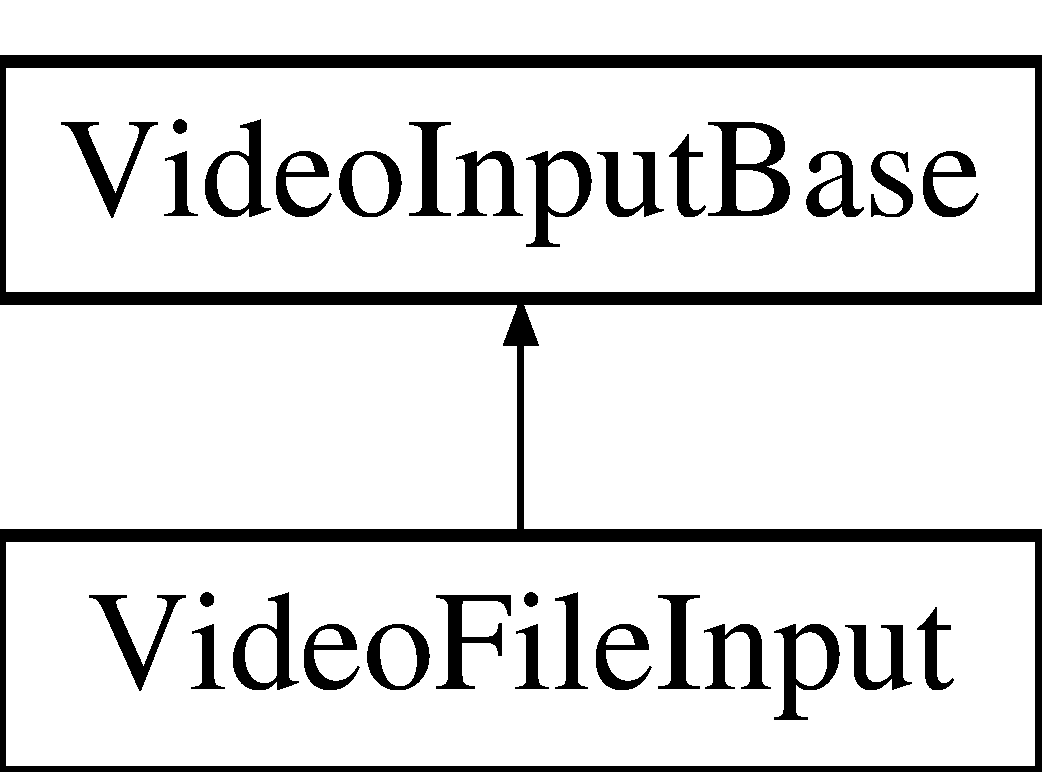
\includegraphics[height=2.000000cm]{class_video_file_input}
\end{center}
\end{figure}
\subsection*{Public Member Functions}
\begin{DoxyCompactItemize}
\item 
\hyperlink{class_video_file_input_af95c920576786bb86b06bb25883747b6}{Video\+File\+Input} (string video\+Config\+File\+Path\+Name)
\begin{DoxyCompactList}\small\item\em Reads in the video\+Config\+File\+Path\+Name to get the location of the video and the inital position and size of the object that we want to track. \end{DoxyCompactList}\item 
void \hyperlink{class_video_file_input_ad2ad075776eed670dcf7e9e372d993cf}{get\+Initial\+Position} (int $\ast$x, int $\ast$y, int $\ast$width, int $\ast$height)
\begin{DoxyCompactList}\small\item\em Gets the initial location of the object that will be tracked. \end{DoxyCompactList}\item 
bool \hyperlink{class_video_file_input_a8d8cc050ab45a3b44403aa53d3d6e697}{start\+Camera} ()
\item 
Mat \hyperlink{class_video_file_input_a937889bfedcff9bd01d22fff70b71a61}{get\+Next\+Frame} ()
\begin{DoxyCompactList}\small\item\em Gets the frame in R\+G\+B colour space. \end{DoxyCompactList}\end{DoxyCompactItemize}
\subsection*{Additional Inherited Members}


\subsection{Detailed Description}
Allows the video feed to come from a video file. 

\subsection{Constructor \& Destructor Documentation}
\hypertarget{class_video_file_input_af95c920576786bb86b06bb25883747b6}{}\index{Video\+File\+Input@{Video\+File\+Input}!Video\+File\+Input@{Video\+File\+Input}}
\index{Video\+File\+Input@{Video\+File\+Input}!Video\+File\+Input@{Video\+File\+Input}}
\subsubsection[{Video\+File\+Input}]{\setlength{\rightskip}{0pt plus 5cm}Video\+File\+Input\+::\+Video\+File\+Input (
\begin{DoxyParamCaption}
\item[{string}]{video\+Config\+File\+Path\+Name}
\end{DoxyParamCaption}
)}\label{class_video_file_input_af95c920576786bb86b06bb25883747b6}


Reads in the video\+Config\+File\+Path\+Name to get the location of the video and the inital position and size of the object that we want to track. 


\begin{DoxyParams}{Parameters}
{\em video\+Config\+File\+Path\+Name} & \mbox{[}in\mbox{]} \\
\hline
\end{DoxyParams}


\subsection{Member Function Documentation}
\hypertarget{class_video_file_input_ad2ad075776eed670dcf7e9e372d993cf}{}\index{Video\+File\+Input@{Video\+File\+Input}!get\+Initial\+Position@{get\+Initial\+Position}}
\index{get\+Initial\+Position@{get\+Initial\+Position}!Video\+File\+Input@{Video\+File\+Input}}
\subsubsection[{get\+Initial\+Position}]{\setlength{\rightskip}{0pt plus 5cm}Video\+File\+Input\+::get\+Initial\+Position (
\begin{DoxyParamCaption}
\item[{int $\ast$}]{x, }
\item[{int $\ast$}]{y, }
\item[{int $\ast$}]{width, }
\item[{int $\ast$}]{height}
\end{DoxyParamCaption}
)}\label{class_video_file_input_ad2ad075776eed670dcf7e9e372d993cf}


Gets the initial location of the object that will be tracked. 


\begin{DoxyParams}{Parameters}
{\em x} & \mbox{[}out\mbox{]} \\
\hline
{\em y} & \mbox{[}out\mbox{]} \\
\hline
{\em width} & \mbox{[}out\mbox{]} \\
\hline
{\em height} & \mbox{[}out\mbox{]} \\
\hline
\end{DoxyParams}
\hypertarget{class_video_file_input_a937889bfedcff9bd01d22fff70b71a61}{}\index{Video\+File\+Input@{Video\+File\+Input}!get\+Next\+Frame@{get\+Next\+Frame}}
\index{get\+Next\+Frame@{get\+Next\+Frame}!Video\+File\+Input@{Video\+File\+Input}}
\subsubsection[{get\+Next\+Frame}]{\setlength{\rightskip}{0pt plus 5cm}Video\+File\+Input\+::get\+Next\+Frame (
\begin{DoxyParamCaption}
{}
\end{DoxyParamCaption}
)\hspace{0.3cm}{\ttfamily [virtual]}}\label{class_video_file_input_a937889bfedcff9bd01d22fff70b71a61}


Gets the frame in R\+G\+B colour space. 

\begin{DoxyReturn}{Returns}
The frame 
\end{DoxyReturn}


Implements \hyperlink{class_video_input_base_a2d289ea71410a736496a180363e219b4}{Video\+Input\+Base}.

\hypertarget{class_video_file_input_a8d8cc050ab45a3b44403aa53d3d6e697}{}\index{Video\+File\+Input@{Video\+File\+Input}!start\+Camera@{start\+Camera}}
\index{start\+Camera@{start\+Camera}!Video\+File\+Input@{Video\+File\+Input}}
\subsubsection[{start\+Camera}]{\setlength{\rightskip}{0pt plus 5cm}Video\+File\+Input\+::start\+Camera (
\begin{DoxyParamCaption}
{}
\end{DoxyParamCaption}
)\hspace{0.3cm}{\ttfamily [virtual]}}\label{class_video_file_input_a8d8cc050ab45a3b44403aa53d3d6e697}
\begin{DoxyReturn}{Returns}
true if camera has successfully been started 
\end{DoxyReturn}


Implements \hyperlink{class_video_input_base_aff0dba9ff7bebd2d6d3fe55bc6f1c0c0}{Video\+Input\+Base}.



The documentation for this class was generated from the following files\+:\begin{DoxyCompactItemize}
\item 
Video\+Device\+Interaction/\hyperlink{video_file_input_8h}{video\+File\+Input.\+h}\item 
Video\+Device\+Interaction/\hyperlink{video_file_input_8cpp}{video\+File\+Input.\+cpp}\end{DoxyCompactItemize}

\hypertarget{class_video_input_base}{}\section{Video\+Input\+Base Class Reference}
\label{class_video_input_base}\index{Video\+Input\+Base@{Video\+Input\+Base}}


This acts as and interface and holds the implementation common to \hyperlink{class_video_file_input}{Video\+File\+Input} and \hyperlink{class_webcam_input}{Webcam\+Input}.  




{\ttfamily \#include $<$video\+Input\+Base.\+h$>$}

Inheritance diagram for Video\+Input\+Base\+:\begin{figure}[H]
\begin{center}
\leavevmode
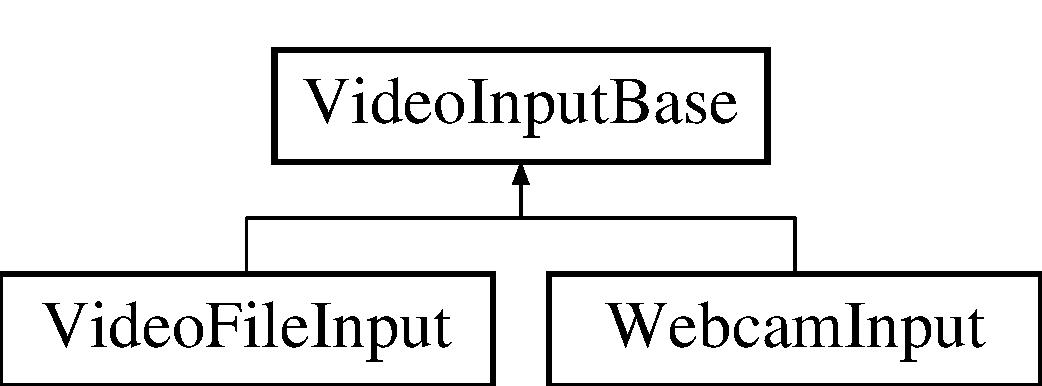
\includegraphics[height=2.000000cm]{class_video_input_base}
\end{center}
\end{figure}
\subsection*{Public Member Functions}
\begin{DoxyCompactItemize}
\item 
virtual bool \hyperlink{class_video_input_base_aff0dba9ff7bebd2d6d3fe55bc6f1c0c0}{start\+Camera} ()=0
\begin{DoxyCompactList}\small\item\em Opens the connection to the webcam. \end{DoxyCompactList}\item 
virtual Mat \hyperlink{class_video_input_base_a2d289ea71410a736496a180363e219b4}{get\+Next\+Frame} ()=0
\begin{DoxyCompactList}\small\item\em Gets the video frame in R\+G\+B colour space. \end{DoxyCompactList}\item 
\hypertarget{class_video_input_base_af2d32b5797e19abe6f1084f81f29554b}{}void \hyperlink{class_video_input_base_af2d32b5797e19abe6f1084f81f29554b}{close} ()\label{class_video_input_base_af2d32b5797e19abe6f1084f81f29554b}

\begin{DoxyCompactList}\small\item\em Closes the connection to the Webcam. \end{DoxyCompactList}\end{DoxyCompactItemize}
\subsection*{Protected Attributes}
\begin{DoxyCompactItemize}
\item 
\hypertarget{class_video_input_base_ac7c36d8f4df7e18c1f8dffa3972a3620}{}const double \hyperlink{class_video_input_base_ac7c36d8f4df7e18c1f8dffa3972a3620}{S\+C\+A\+L\+E\+\_\+\+F\+A\+C\+T\+O\+R} = 0.\+5\label{class_video_input_base_ac7c36d8f4df7e18c1f8dffa3972a3620}

\begin{DoxyCompactList}\small\item\em Video input is too high a resolution to work in real-\/time when using semi-\/exustive appearance matching. \end{DoxyCompactList}\item 
\hypertarget{class_video_input_base_ac780b7966a6d11a890bc7c9ea3103be9}{}Video\+Capture \hyperlink{class_video_input_base_ac780b7966a6d11a890bc7c9ea3103be9}{capture}\label{class_video_input_base_ac780b7966a6d11a890bc7c9ea3103be9}

\begin{DoxyCompactList}\small\item\em The capture object the frame will be read from. \end{DoxyCompactList}\end{DoxyCompactItemize}


\subsection{Detailed Description}
This acts as and interface and holds the implementation common to \hyperlink{class_video_file_input}{Video\+File\+Input} and \hyperlink{class_webcam_input}{Webcam\+Input}. 

\subsection{Member Function Documentation}
\hypertarget{class_video_input_base_a2d289ea71410a736496a180363e219b4}{}\index{Video\+Input\+Base@{Video\+Input\+Base}!get\+Next\+Frame@{get\+Next\+Frame}}
\index{get\+Next\+Frame@{get\+Next\+Frame}!Video\+Input\+Base@{Video\+Input\+Base}}
\subsubsection[{get\+Next\+Frame}]{\setlength{\rightskip}{0pt plus 5cm}Video\+Input\+Base\+::get\+Next\+Frame (
\begin{DoxyParamCaption}
{}
\end{DoxyParamCaption}
)\hspace{0.3cm}{\ttfamily [pure virtual]}}\label{class_video_input_base_a2d289ea71410a736496a180363e219b4}


Gets the video frame in R\+G\+B colour space. 

\begin{DoxyReturn}{Returns}
the video frame 
\end{DoxyReturn}


Implemented in \hyperlink{class_video_file_input_a937889bfedcff9bd01d22fff70b71a61}{Video\+File\+Input}, and \hyperlink{class_webcam_input_a991fd28f2e4e9dd8608becdb4976cfde}{Webcam\+Input}.

\hypertarget{class_video_input_base_aff0dba9ff7bebd2d6d3fe55bc6f1c0c0}{}\index{Video\+Input\+Base@{Video\+Input\+Base}!start\+Camera@{start\+Camera}}
\index{start\+Camera@{start\+Camera}!Video\+Input\+Base@{Video\+Input\+Base}}
\subsubsection[{start\+Camera}]{\setlength{\rightskip}{0pt plus 5cm}Video\+Input\+Base\+::start\+Camera (
\begin{DoxyParamCaption}
{}
\end{DoxyParamCaption}
)\hspace{0.3cm}{\ttfamily [pure virtual]}}\label{class_video_input_base_aff0dba9ff7bebd2d6d3fe55bc6f1c0c0}


Opens the connection to the webcam. 


\begin{DoxyParams}{Parameters}
{\em camera\+Id} & \\
\hline
\end{DoxyParams}
\begin{DoxyReturn}{Returns}
true if the video input has been successfully opened 
\end{DoxyReturn}


Implemented in \hyperlink{class_video_file_input_a8d8cc050ab45a3b44403aa53d3d6e697}{Video\+File\+Input}, and \hyperlink{class_webcam_input_a716c7ae34722a6760bed160a5a127f73}{Webcam\+Input}.



The documentation for this class was generated from the following files\+:\begin{DoxyCompactItemize}
\item 
Video\+Device\+Interaction/video\+Input\+Base.\+h\item 
Video\+Device\+Interaction/\hyperlink{video_input_base_8cpp}{video\+Input\+Base.\+cpp}\end{DoxyCompactItemize}

\hypertarget{class_webcam_input}{}\section{Webcam\+Input Class Reference}
\label{class_webcam_input}\index{Webcam\+Input@{Webcam\+Input}}
Inheritance diagram for Webcam\+Input\+:\begin{figure}[H]
\begin{center}
\leavevmode
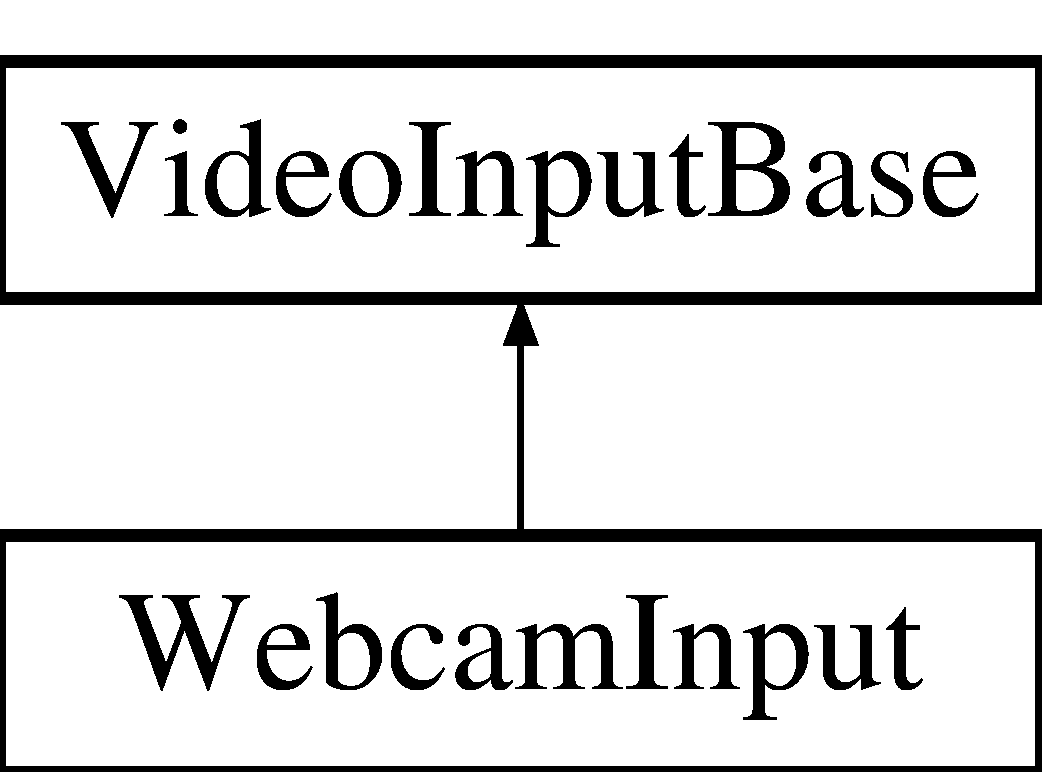
\includegraphics[height=2.000000cm]{class_webcam_input}
\end{center}
\end{figure}
\subsection*{Public Member Functions}
\begin{DoxyCompactItemize}
\item 
bool \hyperlink{class_webcam_input_a716c7ae34722a6760bed160a5a127f73}{start\+Camera} ()
\begin{DoxyCompactList}\small\item\em Opens the video capture device. \end{DoxyCompactList}\item 
Mat \hyperlink{class_webcam_input_a991fd28f2e4e9dd8608becdb4976cfde}{get\+Next\+Frame} ()
\begin{DoxyCompactList}\small\item\em Gets the frame in R\+G\+B colour space. \end{DoxyCompactList}\end{DoxyCompactItemize}
\subsection*{Additional Inherited Members}


\subsection{Member Function Documentation}
\hypertarget{class_webcam_input_a991fd28f2e4e9dd8608becdb4976cfde}{}\index{Webcam\+Input@{Webcam\+Input}!get\+Next\+Frame@{get\+Next\+Frame}}
\index{get\+Next\+Frame@{get\+Next\+Frame}!Webcam\+Input@{Webcam\+Input}}
\subsubsection[{get\+Next\+Frame}]{\setlength{\rightskip}{0pt plus 5cm}Webcam\+Input\+::get\+Next\+Frame (
\begin{DoxyParamCaption}
{}
\end{DoxyParamCaption}
)\hspace{0.3cm}{\ttfamily [virtual]}}\label{class_webcam_input_a991fd28f2e4e9dd8608becdb4976cfde}


Gets the frame in R\+G\+B colour space. 

\begin{DoxyReturn}{Returns}
The camera frame 
\end{DoxyReturn}


Implements \hyperlink{class_video_input_base_a2d289ea71410a736496a180363e219b4}{Video\+Input\+Base}.

\hypertarget{class_webcam_input_a716c7ae34722a6760bed160a5a127f73}{}\index{Webcam\+Input@{Webcam\+Input}!start\+Camera@{start\+Camera}}
\index{start\+Camera@{start\+Camera}!Webcam\+Input@{Webcam\+Input}}
\subsubsection[{start\+Camera}]{\setlength{\rightskip}{0pt plus 5cm}Webcam\+Input\+::start\+Camera (
\begin{DoxyParamCaption}
{}
\end{DoxyParamCaption}
)\hspace{0.3cm}{\ttfamily [virtual]}}\label{class_webcam_input_a716c7ae34722a6760bed160a5a127f73}


Opens the video capture device. 

\begin{DoxyReturn}{Returns}
true if the video input has been successfully opened 
\end{DoxyReturn}


Implements \hyperlink{class_video_input_base_aff0dba9ff7bebd2d6d3fe55bc6f1c0c0}{Video\+Input\+Base}.



The documentation for this class was generated from the following files\+:\begin{DoxyCompactItemize}
\item 
Video\+Device\+Interaction/\hyperlink{webcam_input_8h}{webcam\+Input.\+h}\item 
Video\+Device\+Interaction/\hyperlink{webcam_input_8cpp}{webcam\+Input.\+cpp}\end{DoxyCompactItemize}

\chapter{File Documentation}
\hypertarget{arb_8cpp}{}\section{A\+I\+S/arb.cpp File Reference}
\label{arb_8cpp}\index{A\+I\+S/arb.\+cpp@{A\+I\+S/arb.\+cpp}}


The source code for the \hyperlink{class_a_r_b}{A\+R\+B} class. The decay\+Resource\+Level(), increase\+Resource\+Level() and get\+Stimulation\+Level() are based on the equations in \char`\"{}\+An artificial immune system for continuous analysis of time-\/varying data\char`\"{} by M.\+Neal 2002.  


{\ttfamily \#include \char`\"{}arb.\+h\char`\"{}}\\*


\subsection{Detailed Description}
The source code for the \hyperlink{class_a_r_b}{A\+R\+B} class. The decay\+Resource\+Level(), increase\+Resource\+Level() and get\+Stimulation\+Level() are based on the equations in \char`\"{}\+An artificial immune system for continuous analysis of time-\/varying data\char`\"{} by M.\+Neal 2002. 

\begin{DoxyAuthor}{Author}
Helen Harman (\href{mailto:heh14@aber.ac.uk}{\tt heh14@aber.\+ac.\+uk}) 
\end{DoxyAuthor}
\begin{DoxyDate}{Date}
06/03/2015 
\end{DoxyDate}
\begin{DoxyVersion}{Version}
1.\+0 
\end{DoxyVersion}

\hypertarget{arb_8h}{}\section{A\+I\+S/arb.h File Reference}
\label{arb_8h}\index{A\+I\+S/arb.\+h@{A\+I\+S/arb.\+h}}


Holds the \hyperlink{class_a_r_b}{A\+R\+B} class.  


{\ttfamily \#include $<$iostream$>$}\\*
{\ttfamily \#include $<$vector$>$}\\*
{\ttfamily \#include $<$opencv2/core/core.\+hpp$>$}\\*
\subsection*{Classes}
\begin{DoxyCompactItemize}
\item 
class \hyperlink{class_a_r_b}{A\+R\+B}
\begin{DoxyCompactList}\small\item\em \hyperlink{class_a_r_b}{A\+R\+B}\textquotesingle{}s are the nodes within the network, which contain an appearace of the object. \end{DoxyCompactList}\end{DoxyCompactItemize}


\subsection{Detailed Description}
Holds the \hyperlink{class_a_r_b}{A\+R\+B} class. 

\begin{DoxyAuthor}{Author}
Helen Harman (\href{mailto:heh14@aber.ac.uk}{\tt heh14@aber.\+ac.\+uk}) 
\end{DoxyAuthor}
\begin{DoxyDate}{Date}
06/03/2015 
\end{DoxyDate}
\begin{DoxyVersion}{Version}
1.\+0 
\end{DoxyVersion}

\hypertarget{network_8cpp}{}\section{A\+I\+S/network.cpp File Reference}
\label{network_8cpp}\index{A\+I\+S/network.\+cpp@{A\+I\+S/network.\+cpp}}


The source code for the \hyperlink{class_network}{Network} class.  


{\ttfamily \#include \char`\"{}network.\+h\char`\"{}}\\*


\subsection{Detailed Description}
The source code for the \hyperlink{class_network}{Network} class. 

\begin{DoxyAuthor}{Author}
Helen Harman (\href{mailto:heh14@aber.ac.uk}{\tt heh14@aber.\+ac.\+uk}) 
\end{DoxyAuthor}
\begin{DoxyDate}{Date}
06/03/2015 
\end{DoxyDate}
\begin{DoxyVersion}{Version}
1.\+0 
\end{DoxyVersion}

\hypertarget{network_8h}{}\section{A\+I\+S/network.h File Reference}
\label{network_8h}\index{A\+I\+S/network.\+h@{A\+I\+S/network.\+h}}


Holds the \hyperlink{class_network}{Network} class.  


{\ttfamily \#include $<$iostream$>$}\\*
{\ttfamily \#include $<$vector$>$}\\*
{\ttfamily \#include $<$opencv2/core/core.\+hpp$>$}\\*
{\ttfamily \#include \char`\"{}arb.\+h\char`\"{}}\\*
{\ttfamily \#include \char`\"{}distance\+Base.\+h\char`\"{}}\\*
{\ttfamily \#include \char`\"{}options.\+h\char`\"{}}\\*
\subsection*{Classes}
\begin{DoxyCompactItemize}
\item 
class \hyperlink{class_network}{Network}
\begin{DoxyCompactList}\small\item\em Holds the network of A\+R\+Bs. Handles the adding and removing of A\+R\+Bs. \end{DoxyCompactList}\end{DoxyCompactItemize}


\subsection{Detailed Description}
Holds the \hyperlink{class_network}{Network} class. 

\begin{DoxyAuthor}{Author}
Helen Harman (\href{mailto:heh14@aber.ac.uk}{\tt heh14@aber.\+ac.\+uk}) 
\end{DoxyAuthor}
\begin{DoxyDate}{Date}
06/03/2015 
\end{DoxyDate}
\begin{DoxyVersion}{Version}
1.\+0 
\end{DoxyVersion}

\hypertarget{distance_base_8cpp}{}\section{Distance\+Measures/distance\+Base.cpp File Reference}
\label{distance_base_8cpp}\index{Distance\+Measures/distance\+Base.\+cpp@{Distance\+Measures/distance\+Base.\+cpp}}


The source code for the \hyperlink{class_distance_base}{Distance\+Base} class.  


{\ttfamily \#include \char`\"{}distance\+Base.\+h\char`\"{}}\\*


\subsection{Detailed Description}
The source code for the \hyperlink{class_distance_base}{Distance\+Base} class. 

\begin{DoxyAuthor}{Author}
Helen Harman (\href{mailto:heh14@aber.ac.uk}{\tt heh14@aber.\+ac.\+uk}) 
\end{DoxyAuthor}
\begin{DoxyDate}{Date}
03/04/2015 
\end{DoxyDate}
\begin{DoxyVersion}{Version}
1.\+0 
\end{DoxyVersion}

\hypertarget{euclidean_distance_8cpp}{}\section{Distance\+Measures/euclidean\+Distance.cpp File Reference}
\label{euclidean_distance_8cpp}\index{Distance\+Measures/euclidean\+Distance.\+cpp@{Distance\+Measures/euclidean\+Distance.\+cpp}}


The source code for the \hyperlink{class_euclidean_distance}{Euclidean\+Distance} class.  


{\ttfamily \#include \char`\"{}euclideandistance.\+h\char`\"{}}\\*


\subsection{Detailed Description}
The source code for the \hyperlink{class_euclidean_distance}{Euclidean\+Distance} class. 

\begin{DoxyAuthor}{Author}
Helen Harman (\href{mailto:heh14@aber.ac.uk}{\tt heh14@aber.\+ac.\+uk}) Aberystwyth University 
\end{DoxyAuthor}
\begin{DoxyDate}{Date}
07/03/2015 
\end{DoxyDate}
\begin{DoxyVersion}{Version}
1.\+0 
\end{DoxyVersion}

\hypertarget{euclidean_distance_8h}{}\section{Distance\+Measures/euclidean\+Distance.h File Reference}
\label{euclidean_distance_8h}\index{Distance\+Measures/euclidean\+Distance.\+h@{Distance\+Measures/euclidean\+Distance.\+h}}


Holds the \hyperlink{class_euclidean_distance}{Euclidean\+Distance} class.  


{\ttfamily \#include \char`\"{}distance\+Base.\+h\char`\"{}}\\*
\subsection*{Classes}
\begin{DoxyCompactItemize}
\item 
class \hyperlink{class_euclidean_distance}{Euclidean\+Distance}
\begin{DoxyCompactList}\small\item\em Used to calculate the Euclidean distance between two appearances. \end{DoxyCompactList}\end{DoxyCompactItemize}


\subsection{Detailed Description}
Holds the \hyperlink{class_euclidean_distance}{Euclidean\+Distance} class. 

\begin{DoxyAuthor}{Author}
Helen Harman (\href{mailto:heh14@aber.ac.uk}{\tt heh14@aber.\+ac.\+uk}) Aberystwyth University 
\end{DoxyAuthor}
\begin{DoxyDate}{Date}
07/03/2015 
\end{DoxyDate}
\begin{DoxyVersion}{Version}
1.\+0 
\end{DoxyVersion}

\hypertarget{sum_of_squared_difference_8cpp}{}\section{Distance\+Measures/sum\+Of\+Squared\+Difference.cpp File Reference}
\label{sum_of_squared_difference_8cpp}\index{Distance\+Measures/sum\+Of\+Squared\+Difference.\+cpp@{Distance\+Measures/sum\+Of\+Squared\+Difference.\+cpp}}


The source code for the \hyperlink{class_sum_of_squared_difference}{Sum\+Of\+Squared\+Difference} class.  


{\ttfamily \#include \char`\"{}sum\+Of\+Squared\+Difference.\+h\char`\"{}}\\*


\subsection{Detailed Description}
The source code for the \hyperlink{class_sum_of_squared_difference}{Sum\+Of\+Squared\+Difference} class. 

\begin{DoxyAuthor}{Author}
Helen Harman (\href{mailto:heh14@aber.ac.uk}{\tt heh14@aber.\+ac.\+uk}) 
\end{DoxyAuthor}
\begin{DoxyDate}{Date}
24/03/2015 
\end{DoxyDate}
\begin{DoxyVersion}{Version}
1.\+0 
\end{DoxyVersion}

\hypertarget{sum_of_squared_difference_8h}{}\section{Distance\+Measures/sum\+Of\+Squared\+Difference.h File Reference}
\label{sum_of_squared_difference_8h}\index{Distance\+Measures/sum\+Of\+Squared\+Difference.\+h@{Distance\+Measures/sum\+Of\+Squared\+Difference.\+h}}


Holds the \hyperlink{class_sum_of_squared_difference}{Sum\+Of\+Squared\+Difference} class.  


{\ttfamily \#include \char`\"{}distance\+Base.\+h\char`\"{}}\\*
\subsection*{Classes}
\begin{DoxyCompactItemize}
\item 
class \hyperlink{class_sum_of_squared_difference}{Sum\+Of\+Squared\+Difference}
\begin{DoxyCompactList}\small\item\em Used to calculate the Sum Of Squared Difference between two appearances. \end{DoxyCompactList}\end{DoxyCompactItemize}


\subsection{Detailed Description}
Holds the \hyperlink{class_sum_of_squared_difference}{Sum\+Of\+Squared\+Difference} class. 

\begin{DoxyAuthor}{Author}
Helen Harman (\href{mailto:heh14@aber.ac.uk}{\tt heh14@aber.\+ac.\+uk}) 
\end{DoxyAuthor}
\begin{DoxyDate}{Date}
24/03/2015 
\end{DoxyDate}
\begin{DoxyVersion}{Version}
1.\+0 
\end{DoxyVersion}

\hypertarget{link_tracking_and_ui_8cpp}{}\section{link\+Tracking\+And\+Ui.\+cpp File Reference}
\label{link_tracking_and_ui_8cpp}\index{link\+Tracking\+And\+Ui.\+cpp@{link\+Tracking\+And\+Ui.\+cpp}}


The source code for the \hyperlink{class_link_tracking_and_ui}{Link\+Tracking\+And\+Ui} class.  


{\ttfamily \#include \char`\"{}link\+Tracking\+And\+Ui.\+h\char`\"{}}\\*


\subsection{Detailed Description}
The source code for the \hyperlink{class_link_tracking_and_ui}{Link\+Tracking\+And\+Ui} class. 

\begin{DoxyAuthor}{Author}
Helen Harman (\href{mailto:heh14@aber.ac.uk}{\tt heh14@aber.\+ac.\+uk}) 
\end{DoxyAuthor}
\begin{DoxyDate}{Date}
12/03/2015 
\end{DoxyDate}
\begin{DoxyVersion}{Version}
1.\+0 
\end{DoxyVersion}

\hypertarget{link_tracking_and_ui_8h}{}\section{link\+Tracking\+And\+Ui.\+h File Reference}
\label{link_tracking_and_ui_8h}\index{link\+Tracking\+And\+Ui.\+h@{link\+Tracking\+And\+Ui.\+h}}


Holds the \hyperlink{class_link_tracking_and_ui}{Link\+Tracking\+And\+Ui} class.  


{\ttfamily \#include \char`\"{}qt\+Widget\+Image\+Display.\+h\char`\"{}}\\*
{\ttfamily \#include \char`\"{}tracking\+And\+Detection.\+h\char`\"{}}\\*
\subsection*{Classes}
\begin{DoxyCompactItemize}
\item 
class \hyperlink{class_link_tracking_and_ui}{Link\+Tracking\+And\+Ui}
\begin{DoxyCompactList}\small\item\em Links the backend tracking code to the front end (U\+I) code. \end{DoxyCompactList}\end{DoxyCompactItemize}


\subsection{Detailed Description}
Holds the \hyperlink{class_link_tracking_and_ui}{Link\+Tracking\+And\+Ui} class. 

\begin{DoxyAuthor}{Author}
Helen Harman (\href{mailto:heh14@aber.ac.uk}{\tt heh14@aber.\+ac.\+uk}) 
\end{DoxyAuthor}
\begin{DoxyDate}{Date}
12/03/2015 
\end{DoxyDate}
\begin{DoxyVersion}{Version}
1.\+0 
\end{DoxyVersion}

\hypertarget{main_8cpp}{}\section{main.\+cpp File Reference}
\label{main_8cpp}\index{main.\+cpp@{main.\+cpp}}
{\ttfamily \#include $<$Q\+Application$>$}\\*
{\ttfamily \#include \char`\"{}mainwindow.\+h\char`\"{}}\\*
{\ttfamily \#include \char`\"{}tracking\+And\+Detection.\+h\char`\"{}}\\*
{\ttfamily \#include \char`\"{}link\+Tracking\+And\+Ui.\+h\char`\"{}}\\*
\subsection*{Functions}
\begin{DoxyCompactItemize}
\item 
\hypertarget{main_8cpp_a0ddf1224851353fc92bfbff6f499fa97}{}int {\bfseries main} (int argc, char $\ast$argv\mbox{[}$\,$\mbox{]})\label{main_8cpp_a0ddf1224851353fc92bfbff6f499fa97}

\end{DoxyCompactItemize}


\subsection{Detailed Description}
\begin{DoxyAuthor}{Author}
Helen Harman (\href{mailto:heh14@aber.ac.uk}{\tt heh14@aber.\+ac.\+uk}) Aberystwyth University 
\end{DoxyAuthor}
\begin{DoxyDate}{Date}
06/03/2015 
\end{DoxyDate}
\begin{DoxyVersion}{Version}
1.\+0 
\end{DoxyVersion}

\hypertarget{options_8h}{}\section{options.\+h File Reference}
\label{options_8h}\index{options.\+h@{options.\+h}}


Holds the enums and structs.  


\subsection*{Classes}
\begin{DoxyCompactItemize}
\item 
struct \hyperlink{struct_a_i_s___options_1_1_location}{A\+I\+S\+\_\+\+Options\+::\+Location}
\end{DoxyCompactItemize}
\subsection*{Enumerations}
\begin{DoxyCompactItemize}
\item 
\hypertarget{namespace_a_i_s___options_ae22a9712f644667e6f3a302f9194f019}{}enum {\bfseries Program\+State} \{ {\bfseries U\+N\+I\+N\+I\+T\+I\+A\+L\+I\+S\+E\+D}, 
{\bfseries S\+E\+L\+E\+C\+T\+I\+N\+G}, 
{\bfseries T\+R\+A\+C\+K\+I\+N\+G}
 \}\label{namespace_a_i_s___options_ae22a9712f644667e6f3a302f9194f019}

\begin{DoxyCompactList}\small\item\em Allows the \hyperlink{class_tracking_and_detection}{Tracking\+And\+Detection} class and the U\+I to know the state of the system. \end{DoxyCompactList}\item 
\hypertarget{namespace_a_i_s___options_a803e9e6dc656e624f2234589d99fc979}{}enum {\bfseries Video\+Input\+Type} \{ {\bfseries W\+E\+B\+C\+A\+M}, 
{\bfseries F\+I\+L\+E\+\_\+\+I\+N\+P\+U\+T}
 \}\label{namespace_a_i_s___options_a803e9e6dc656e624f2234589d99fc979}

\item 
\hypertarget{namespace_a_i_s___options_ab48ef16213939e22c5ae5dee1786aca8}{}enum {\bfseries Distance\+Measure\+Type} \{ {\bfseries E\+U\+C\+L\+I\+D\+E\+A\+N\+\_\+\+D\+I\+S\+T\+A\+N\+C\+E}, 
{\bfseries S\+U\+M\+\_\+\+O\+F\+\_\+\+S\+Q\+U\+A\+R\+E\+D\+\_\+\+D\+I\+F\+F\+E\+R\+E\+N\+C\+E}
 \}\label{namespace_a_i_s___options_ab48ef16213939e22c5ae5dee1786aca8}

\item 
\hypertarget{namespace_a_i_s___options_af45e8577962cb67801a331a7064dc938}{}enum {\bfseries A\+R\+Bs\+To\+Search\+With} \{ {\bfseries A\+L\+L}, 
{\bfseries A\+B\+O\+V\+E\+\_\+\+A\+V\+E\+R\+A\+G\+E}, 
{\bfseries L\+A\+S\+T\+\_\+\+A\+N\+D\+\_\+\+H\+I\+G\+H\+E\+S\+T}
 \}\label{namespace_a_i_s___options_af45e8577962cb67801a331a7064dc938}

\end{DoxyCompactItemize}


\subsection{Detailed Description}
Holds the enums and structs. 

\begin{DoxyAuthor}{Author}
Helen Harman (\href{mailto:heh14@aber.ac.uk}{\tt heh14@aber.\+ac.\+uk}) 
\end{DoxyAuthor}
\begin{DoxyDate}{Date}
10/03/2015 
\end{DoxyDate}
\begin{DoxyVersion}{Version}
1.\+0 
\end{DoxyVersion}

\hypertarget{tracking_and_detection_8cpp}{}\section{tracking\+And\+Detection.\+cpp File Reference}
\label{tracking_and_detection_8cpp}\index{tracking\+And\+Detection.\+cpp@{tracking\+And\+Detection.\+cpp}}


The source code for the \hyperlink{class_tracking_and_detection}{Tracking\+And\+Detection} class.  


{\ttfamily \#include \char`\"{}tracking\+And\+Detection.\+h\char`\"{}}\\*


\subsection{Detailed Description}
The source code for the \hyperlink{class_tracking_and_detection}{Tracking\+And\+Detection} class. 

\begin{DoxyAuthor}{Author}
Helen Harman (\href{mailto:heh14@aber.ac.uk}{\tt heh14@aber.\+ac.\+uk}) 
\end{DoxyAuthor}
\begin{DoxyDate}{Date}
12/03/2015 
\end{DoxyDate}
\begin{DoxyVersion}{Version}
1.\+0 
\end{DoxyVersion}

\hypertarget{tracking_and_detection_8h}{}\section{tracking\+And\+Detection.\+h File Reference}
\label{tracking_and_detection_8h}\index{tracking\+And\+Detection.\+h@{tracking\+And\+Detection.\+h}}


Holds the \hyperlink{class_tracking_and_detection}{Tracking\+And\+Detection} class.  


{\ttfamily \#include $<$iostream$>$}\\*
{\ttfamily \#include $<$cmath$>$}\\*
{\ttfamily \#include $<$qthread.\+h$>$}\\*
{\ttfamily \#include $<$qtimer.\+h$>$}\\*
{\ttfamily \#include \char`\"{}video\+Input\+Base.\+h\char`\"{}}\\*
{\ttfamily \#include \char`\"{}webcam\+Input.\+h\char`\"{}}\\*
{\ttfamily \#include \char`\"{}video\+File\+Input.\+h\char`\"{}}\\*
{\ttfamily \#include \char`\"{}network.\+h\char`\"{}}\\*
{\ttfamily \#include \char`\"{}euclidean\+Distance.\+h\char`\"{}}\\*
{\ttfamily \#include \char`\"{}sum\+Of\+Squared\+Difference.\+h\char`\"{}}\\*
{\ttfamily \#include \char`\"{}options.\+h\char`\"{}}\\*
{\ttfamily \#include \char`\"{}simplex\+Object\+Detector.\+h\char`\"{}}\\*
\subsection*{Classes}
\begin{DoxyCompactItemize}
\item 
class \hyperlink{class_tracking_and_detection}{Tracking\+And\+Detection}
\begin{DoxyCompactList}\small\item\em The class that handles and runs the tracking and detection of an object. \end{DoxyCompactList}\end{DoxyCompactItemize}


\subsection{Detailed Description}
Holds the \hyperlink{class_tracking_and_detection}{Tracking\+And\+Detection} class. 

\begin{DoxyAuthor}{Author}
Helen Harman (\href{mailto:heh14@aber.ac.uk}{\tt heh14@aber.\+ac.\+uk}) 
\end{DoxyAuthor}
\begin{DoxyDate}{Date}
12/03/2015 
\end{DoxyDate}
\begin{DoxyVersion}{Version}
1.\+0 
\end{DoxyVersion}

\hypertarget{transformations_8h}{}\section{transformations.\+h File Reference}
\label{transformations_8h}\index{transformations.\+h@{transformations.\+h}}


The source code for the \hyperlink{class_transformations}{Transformations} class.  


{\ttfamily \#include $<$math.\+h$>$}\\*
{\ttfamily \#include $<$opencv2/core/core.\+hpp$>$}\\*
{\ttfamily \#include $<$opencv2/imgproc/imgproc.\+hpp$>$}\\*
{\ttfamily \#include $<$opencv2/highgui/highgui.\+hpp$>$}\\*
\subsection*{Classes}
\begin{DoxyCompactItemize}
\item 
class \hyperlink{class_transformations}{Transformations}
\begin{DoxyCompactList}\small\item\em Performs the rotation of a position and an image. Stopped code being repeated in several places. \end{DoxyCompactList}\end{DoxyCompactItemize}


\subsection{Detailed Description}
The source code for the \hyperlink{class_transformations}{Transformations} class. 

Holds the \hyperlink{class_transformations}{Transformations} class.

\begin{DoxyAuthor}{Author}
Helen Harman (\href{mailto:heh14@aber.ac.uk}{\tt heh14@aber.\+ac.\+uk}) Aberystwyth University 
\end{DoxyAuthor}
\begin{DoxyDate}{Date}
30/03/2015 
\end{DoxyDate}
\begin{DoxyVersion}{Version}
1.\+0 
\end{DoxyVersion}

\hypertarget{mainwindow_8cpp}{}\section{U\+I/mainwindow.cpp File Reference}
\label{mainwindow_8cpp}\index{U\+I/mainwindow.\+cpp@{U\+I/mainwindow.\+cpp}}


The source code for the \hyperlink{class_main_window}{Main\+Window} class.  


{\ttfamily \#include \char`\"{}mainwindow.\+h\char`\"{}}\\*
{\ttfamily \#include \char`\"{}ui\+\_\+mainwindow.\+h\char`\"{}}\\*


\subsection{Detailed Description}
The source code for the \hyperlink{class_main_window}{Main\+Window} class. 

\begin{DoxyAuthor}{Author}
Helen Harman (\href{mailto:heh14@aber.ac.uk}{\tt heh14@aber.\+ac.\+uk}) 
\end{DoxyAuthor}
\begin{DoxyDate}{Date}
06/03/2015 
\end{DoxyDate}
\begin{DoxyVersion}{Version}
1.\+0 
\end{DoxyVersion}

\hypertarget{mainwindow_8h}{}\section{U\+I/mainwindow.h File Reference}
\label{mainwindow_8h}\index{U\+I/mainwindow.\+h@{U\+I/mainwindow.\+h}}


Holds the \hyperlink{class_main_window}{Main\+Window} class.  


{\ttfamily \#include $<$Q\+Main\+Window$>$}\\*
{\ttfamily \#include $<$Q\+Input\+Dialog$>$}\\*
{\ttfamily \#include \char`\"{}qt\+Widget\+Image\+Display.\+h\char`\"{}}\\*
\subsection*{Classes}
\begin{DoxyCompactItemize}
\item 
class \hyperlink{class_main_window}{Main\+Window}
\begin{DoxyCompactList}\small\item\em The main U\+I window. \end{DoxyCompactList}\end{DoxyCompactItemize}


\subsection{Detailed Description}
Holds the \hyperlink{class_main_window}{Main\+Window} class. 

\begin{DoxyAuthor}{Author}
Helen Harman (\href{mailto:heh14@aber.ac.uk}{\tt heh14@aber.\+ac.\+uk}) 
\end{DoxyAuthor}
\begin{DoxyDate}{Date}
06/03/2015 
\end{DoxyDate}
\begin{DoxyVersion}{Version}
1.\+0 
\end{DoxyVersion}

\hypertarget{output_data_8cpp}{}\section{U\+I/output\+Data.cpp File Reference}
\label{output_data_8cpp}\index{U\+I/output\+Data.\+cpp@{U\+I/output\+Data.\+cpp}}


The source code for the \hyperlink{class_output_data}{Output\+Data} class.  


{\ttfamily \#include \char`\"{}output\+Data.\+h\char`\"{}}\\*


\subsection{Detailed Description}
The source code for the \hyperlink{class_output_data}{Output\+Data} class. 

\begin{DoxyAuthor}{Author}
Helen Harman (\href{mailto:heh14@aber.ac.uk}{\tt heh14@aber.\+ac.\+uk}) 
\end{DoxyAuthor}
\begin{DoxyDate}{Date}
06/03/2015 
\end{DoxyDate}
\begin{DoxyVersion}{Version}
1.\+0 
\end{DoxyVersion}

\hypertarget{qt_widget_image_display_8cpp}{}\section{U\+I/qt\+Widget\+Image\+Display.cpp File Reference}
\label{qt_widget_image_display_8cpp}\index{U\+I/qt\+Widget\+Image\+Display.\+cpp@{U\+I/qt\+Widget\+Image\+Display.\+cpp}}


The source code for the \hyperlink{class_qt_widget_image_display}{Qt\+Widget\+Image\+Display} class.  


{\ttfamily \#include \char`\"{}qt\+Widget\+Image\+Display.\+h\char`\"{}}\\*


\subsection{Detailed Description}
The source code for the \hyperlink{class_qt_widget_image_display}{Qt\+Widget\+Image\+Display} class. 

\begin{DoxyAuthor}{Author}
Helen Harman (\href{mailto:heh14@aber.ac.uk}{\tt heh14@aber.\+ac.\+uk}) 
\end{DoxyAuthor}
\begin{DoxyDate}{Date}
12/03/2015 
\end{DoxyDate}
\begin{DoxyVersion}{Version}
1.\+0 
\end{DoxyVersion}

\hypertarget{qt_widget_image_display_8h}{}\section{U\+I/qt\+Widget\+Image\+Display.h File Reference}
\label{qt_widget_image_display_8h}\index{U\+I/qt\+Widget\+Image\+Display.\+h@{U\+I/qt\+Widget\+Image\+Display.\+h}}


Holds the \hyperlink{class_qt_widget_image_display}{Qt\+Widget\+Image\+Display} class Made use of \href{http://develnoter.blogspot.co.uk/2012/05/integrating-opencv-in-qt-gui.html}{\tt http\+://develnoter.\+blogspot.\+co.\+uk/2012/05/integrating-\/opencv-\/in-\/qt-\/gui.\+html} (Marcelo Mottalli, 2012 \mbox{[}Accessed \+: April 2015\mbox{]}) to learn how to show a Open\+C\+V Mat image in a Qt window.  


{\ttfamily \#include $<$iostream$>$}\\*
{\ttfamily \#include $<$Q\+File\+Dialog$>$}\\*
{\ttfamily \#include $<$Q\+Widget$>$}\\*
{\ttfamily \#include $<$Q\+Image$>$}\\*
{\ttfamily \#include $<$Q\+Painter$>$}\\*
{\ttfamily \#include $<$Q\+Mouse\+Event$>$}\\*
{\ttfamily \#include $<$opencv2/core/core.\+hpp$>$}\\*
{\ttfamily \#include \char`\"{}options.\+h\char`\"{}}\\*
{\ttfamily \#include \char`\"{}transformations.\+h\char`\"{}}\\*
{\ttfamily \#include \char`\"{}output\+Data.\+h\char`\"{}}\\*
\subsection*{Classes}
\begin{DoxyCompactItemize}
\item 
class \hyperlink{class_qt_widget_image_display}{Qt\+Widget\+Image\+Display}
\begin{DoxyCompactList}\small\item\em Allows the video to be displayed and shows the position of the object being tracked. \end{DoxyCompactList}\end{DoxyCompactItemize}


\subsection{Detailed Description}
Holds the \hyperlink{class_qt_widget_image_display}{Qt\+Widget\+Image\+Display} class Made use of \href{http://develnoter.blogspot.co.uk/2012/05/integrating-opencv-in-qt-gui.html}{\tt http\+://develnoter.\+blogspot.\+co.\+uk/2012/05/integrating-\/opencv-\/in-\/qt-\/gui.\+html} (Marcelo Mottalli, 2012 \mbox{[}Accessed \+: April 2015\mbox{]}) to learn how to show a Open\+C\+V Mat image in a Qt window. 

\begin{DoxyAuthor}{Author}
Helen Harman (\href{mailto:heh14@aber.ac.uk}{\tt heh14@aber.\+ac.\+uk}) 
\end{DoxyAuthor}
\begin{DoxyDate}{Date}
12/03/2015 
\end{DoxyDate}
\begin{DoxyVersion}{Version}
1.\+0 
\end{DoxyVersion}

\hypertarget{video_file_input_8cpp}{}\section{Video\+Device\+Interaction/video\+File\+Input.cpp File Reference}
\label{video_file_input_8cpp}\index{Video\+Device\+Interaction/video\+File\+Input.\+cpp@{Video\+Device\+Interaction/video\+File\+Input.\+cpp}}


The source code for the \hyperlink{class_video_file_input}{Video\+File\+Input} class.  


{\ttfamily \#include \char`\"{}video\+File\+Input.\+h\char`\"{}}\\*


\subsection{Detailed Description}
The source code for the \hyperlink{class_video_file_input}{Video\+File\+Input} class. 

\begin{DoxyAuthor}{Author}
Helen Harman (\href{mailto:heh14@aber.ac.uk}{\tt heh14@aber.\+ac.\+uk}) 
\end{DoxyAuthor}
\begin{DoxyDate}{Date}
13/03/2015 
\end{DoxyDate}
\begin{DoxyVersion}{Version}
1.\+0 
\end{DoxyVersion}

\hypertarget{video_file_input_8h}{}\section{Video\+Device\+Interaction/video\+File\+Input.h File Reference}
\label{video_file_input_8h}\index{Video\+Device\+Interaction/video\+File\+Input.\+h@{Video\+Device\+Interaction/video\+File\+Input.\+h}}


Holds the \hyperlink{class_video_file_input}{Video\+File\+Input} class.  


{\ttfamily \#include $<$fstream$>$}\\*
{\ttfamily \#include \char`\"{}video\+Input\+Base.\+h\char`\"{}}\\*
\subsection*{Classes}
\begin{DoxyCompactItemize}
\item 
class \hyperlink{class_video_file_input}{Video\+File\+Input}
\begin{DoxyCompactList}\small\item\em Allows the video feed to come from a video file. \end{DoxyCompactList}\end{DoxyCompactItemize}


\subsection{Detailed Description}
Holds the \hyperlink{class_video_file_input}{Video\+File\+Input} class. 

\begin{DoxyAuthor}{Author}
Helen Harman (\href{mailto:heh14@aber.ac.uk}{\tt heh14@aber.\+ac.\+uk}) 
\end{DoxyAuthor}
\begin{DoxyDate}{Date}
13/03/2015 
\end{DoxyDate}
\begin{DoxyVersion}{Version}
1.\+0 
\end{DoxyVersion}

\hypertarget{video_input_base_8cpp}{}\section{Video\+Device\+Interaction/video\+Input\+Base.cpp File Reference}
\label{video_input_base_8cpp}\index{Video\+Device\+Interaction/video\+Input\+Base.\+cpp@{Video\+Device\+Interaction/video\+Input\+Base.\+cpp}}


The source code for the \hyperlink{class_video_input_base}{Video\+Input\+Base} class.  


{\ttfamily \#include \char`\"{}video\+Input\+Base.\+h\char`\"{}}\\*


\subsection{Detailed Description}
The source code for the \hyperlink{class_video_input_base}{Video\+Input\+Base} class. 

Holds the \hyperlink{class_video_input_base}{Video\+Input\+Base} class.

\begin{DoxyAuthor}{Author}
Helen Harman (\href{mailto:heh14@aber.ac.uk}{\tt heh14@aber.\+ac.\+uk}) 
\end{DoxyAuthor}
\begin{DoxyDate}{Date}
03/04/2015 
\end{DoxyDate}
\begin{DoxyVersion}{Version}
1.\+0
\end{DoxyVersion}
\begin{DoxyAuthor}{Author}
Helen Harman (\href{mailto:heh14@aber.ac.uk}{\tt heh14@aber.\+ac.\+uk}) 
\end{DoxyAuthor}
\begin{DoxyDate}{Date}
06/03/2015 
\end{DoxyDate}
\begin{DoxyVersion}{Version}
1.\+0 
\end{DoxyVersion}

\hypertarget{webcam_input_8cpp}{}\section{Video\+Device\+Interaction/webcam\+Input.cpp File Reference}
\label{webcam_input_8cpp}\index{Video\+Device\+Interaction/webcam\+Input.\+cpp@{Video\+Device\+Interaction/webcam\+Input.\+cpp}}


The source code for the \hyperlink{class_webcam_input}{Webcam\+Input} class.  


{\ttfamily \#include \char`\"{}webcaminput.\+h\char`\"{}}\\*


\subsection{Detailed Description}
The source code for the \hyperlink{class_webcam_input}{Webcam\+Input} class. 

\begin{DoxyAuthor}{Author}
Helen Harman (\href{mailto:heh14@aber.ac.uk}{\tt heh14@aber.\+ac.\+uk}) 
\end{DoxyAuthor}
\begin{DoxyDate}{Date}
06/03/2015 
\end{DoxyDate}
\begin{DoxyVersion}{Version}
1.\+0 
\end{DoxyVersion}

\hypertarget{webcam_input_8h}{}\section{Video\+Device\+Interaction/webcam\+Input.h File Reference}
\label{webcam_input_8h}\index{Video\+Device\+Interaction/webcam\+Input.\+h@{Video\+Device\+Interaction/webcam\+Input.\+h}}


Holds the \hyperlink{class_webcam_input}{Webcam\+Input} class.  


{\ttfamily \#include $<$iostream$>$}\\*
{\ttfamily \#include \char`\"{}video\+Input\+Base.\+h\char`\"{}}\\*
\subsection*{Classes}
\begin{DoxyCompactItemize}
\item 
class \hyperlink{class_webcam_input}{Webcam\+Input}
\end{DoxyCompactItemize}


\subsection{Detailed Description}
Holds the \hyperlink{class_webcam_input}{Webcam\+Input} class. 

\begin{DoxyAuthor}{Author}
Helen Harman (\href{mailto:heh14@aber.ac.uk}{\tt heh14@aber.\+ac.\+uk}) 
\end{DoxyAuthor}
\begin{DoxyDate}{Date}
06/03/2015 
\end{DoxyDate}
\begin{DoxyVersion}{Version}
1.\+0 
\end{DoxyVersion}

%--- End generated contents ---

% Index
\backmatter
\newpage
\phantomsection
\clearemptydoublepage
\addcontentsline{toc}{chapter}{Index}
\printindex

\end{document}
